\chapter{Calorimeter Optimisation Studies}
\label{chap:detopt}

\chapterquote{The simple believes everything, but the prudent gives thought to his steps.}
{Proverbs 14:15}

%========================================================================================
%========================================================================================

\section{Introduction}
\label{sec:optimisationstudies}
This chapter considered optimisation of the calorimeters used at the linear collider, with focus placed on obtaining the best energy resolution for jets.  Parameters such as the number of layers, cell size and material choices for the calorimeters are investigated.  This chapter concludes with an optimisation of several global detector parameters such as the magnetic field strength and the inner radius of the ECal.  These parameters are not calorimeter specific, but affect the jet energy resolution obtained from particle flow. 

The nominal detector model used in these optimisation studies is the ILD detector model, which is discussed in detail in section \ref{sec:ild}.  A description of the metrics used to quantify detector performance in this chapter can be found in section \ref{sec:performance}.  A summary of the performance of the nominal ILD detector model is given in section \ref{sec:nominaldetectorperformance}.

%========================================================================================
%========================================================================================

\section{Electromagnetic Calorimeter Optimisation}
\label{sec:ecal}
The purpose of an electromagnetic calorimeter (ECal) is to measures the energy deposits from electromagnetic showers.  The nominal ILD detector model ECal, summarised in table \ref{table:defaultildecal}, is a silicon-tungsten sampling calorimeter.  It contains 29 readout layers and 24 radiation lengths ($\text{X}_{0}$), which is sufficient to contain all but the highest energy electromagnetic showers.  The absorber thickness of the last nine layers is twice that of the first 20 layers to reduce the number of readout channels and cost of the calorimeter.  This high sampling rate is crucial for the pattern recognition aspect of particle flow calorimetry, especially in the region where particle showers start developing, as shown in section \ref{sec:ecalcells}.  

\begin{table}[h!]
\centering
\begin{tabular}{ l l}
\hline
Parameter & Default Value \\
\hline
Cell Size & $5 \times 5 \text{mm}^{2}$ square cells \\
Number of Layers & 29 readout layers \\
Active Material Choice & Silicon or Scintillator  \\
Active Material Thickness & 0.5 mm (Silicon) or 2 mm (Scintillator)  \\
Absorber Material Choice & Tungsten \\
Absorber Material Thickness & 20 layers of 2.1 mm followed by 9 layers of 4.2 mm \\
\hline
\end{tabular}
\caption[The configuration of the ECal in the nominal ILD detector model.  The parameters are given for the nominal silicon model as well as the alternative scintillator option.]{The configuration of the ECal in the nominal ILD detector model.  The parameters are given for the nominal silicon model as well as the alternative scintillator option.}
\label{table:defaultildecal}
\end{table}

The calorimeter performance was simulated for a number of detector models where the following detector parameters were varied:
\begin{itemize}
\item Cell size:  This is a vital aspect of the detector in the particle flow paradigm as smaller cell sizes leads to better separation between nearby showering particles, which helps to minimise the effect of confusion.  Modifying the cell size should have little effect on the intrinsic energy resolution of the detector.  
\item Sampling frequency:  The sampling frequency in the ECal was varied by changing the number of layers in the ECal while simultaneously changing the thicknesses of the layers such that the total depth, in radiation lengths, was held constant.  Increasing the number of layers in a sampling calorimeter means any particles showering within it are sampled more thoroughly.  This leads to a reduction in the stochastic contribution to the energy resolution, as discussed in section \ref{sec:nominaldetectorperformance}.  Therefore, varying the number of layers is expected to change in intrinsic energy resolution of the calorimeter.  
\item Active material choice:  The options under consideration for the active material choice are silicon or scintillator.  As well as providing different intrinsic energy resolutions the readout mechanics of these two options are significantly different.  There is no clear prior knowledge as to which should provide better performance. 
\end{itemize}

%========================================================================================

\subsection{ECal Cell Size}
\label{sec:ecalcells}
A number of different detector models were considered where the cell size in the ECal was varied about the nominal value of $5 \times 5 \text{mm}^{2}$ square cells.  The granularities considered were $3 \times 3 \text{mm}^{2}$, $5 \times 5 \text{mm}^{2}$, $7 \times 7 \text{mm}^{2}$, $10 \times 10 \text{mm}^{2}$, $15 \times 15 \text{mm}^{2}$ and $20 \times 20 \text{mm}^{2}$ square cells for both the silicon and scintillator active material options.  

The energy resolution, using 100~GeV $\gamma$ events, as a function of the ECal cell size is shown in figure \ref{fig:ecalsicellsize} for the silicon option and figure \ref{fig:ecalsccellsize} for the scintillator option.  As, at these energies, the $\gamma$s will be largely contained within the ECal, these results solely reflect the performance of the ECal.  For both the silicon and scintillator ECal options the energy resolution does not depend strongly on the ECal cell size.  This is to be expected as the number of layers, which is the main factor in determining the energy resolution of a sampling calorimeter, does not change when modifying the cell size.  There are minor fluctuations in the energy resolution when varying the cell size, but these are mostly likely due to fluctuations in the energy response from calibration procedure applied to each detector models.  For the scintillator ECal option there is a significant degradation in the energy resolution for the $3 \times 3 \text{mm}^{2}$ cell size model.  The most likely cause of this is a "dead" region in the active material, which represents the readout multi pixel photon counter (MPPC) \cite{arXiv:1006.3396}.  The MPPC occupies a fixed area of the cell, irrespective of cell size, and so the dead region of the cell fractionally increases as cell size is reduced.  The larger this dead region, the worse the sampling of the electromagnetic showers in the ECal and the worse the resolution.  While this effect will be present in all scintillator ECal options, it will only be significant for the small cell sizes when the dead region is fractionally the largest.  This explains why degradation is seen only for the smallest cell size considered in the scintillator ECal option.     

\begin{figure}[h!]
\centering
\subfloat[]{\label{fig:ecalsicellsize100gamma}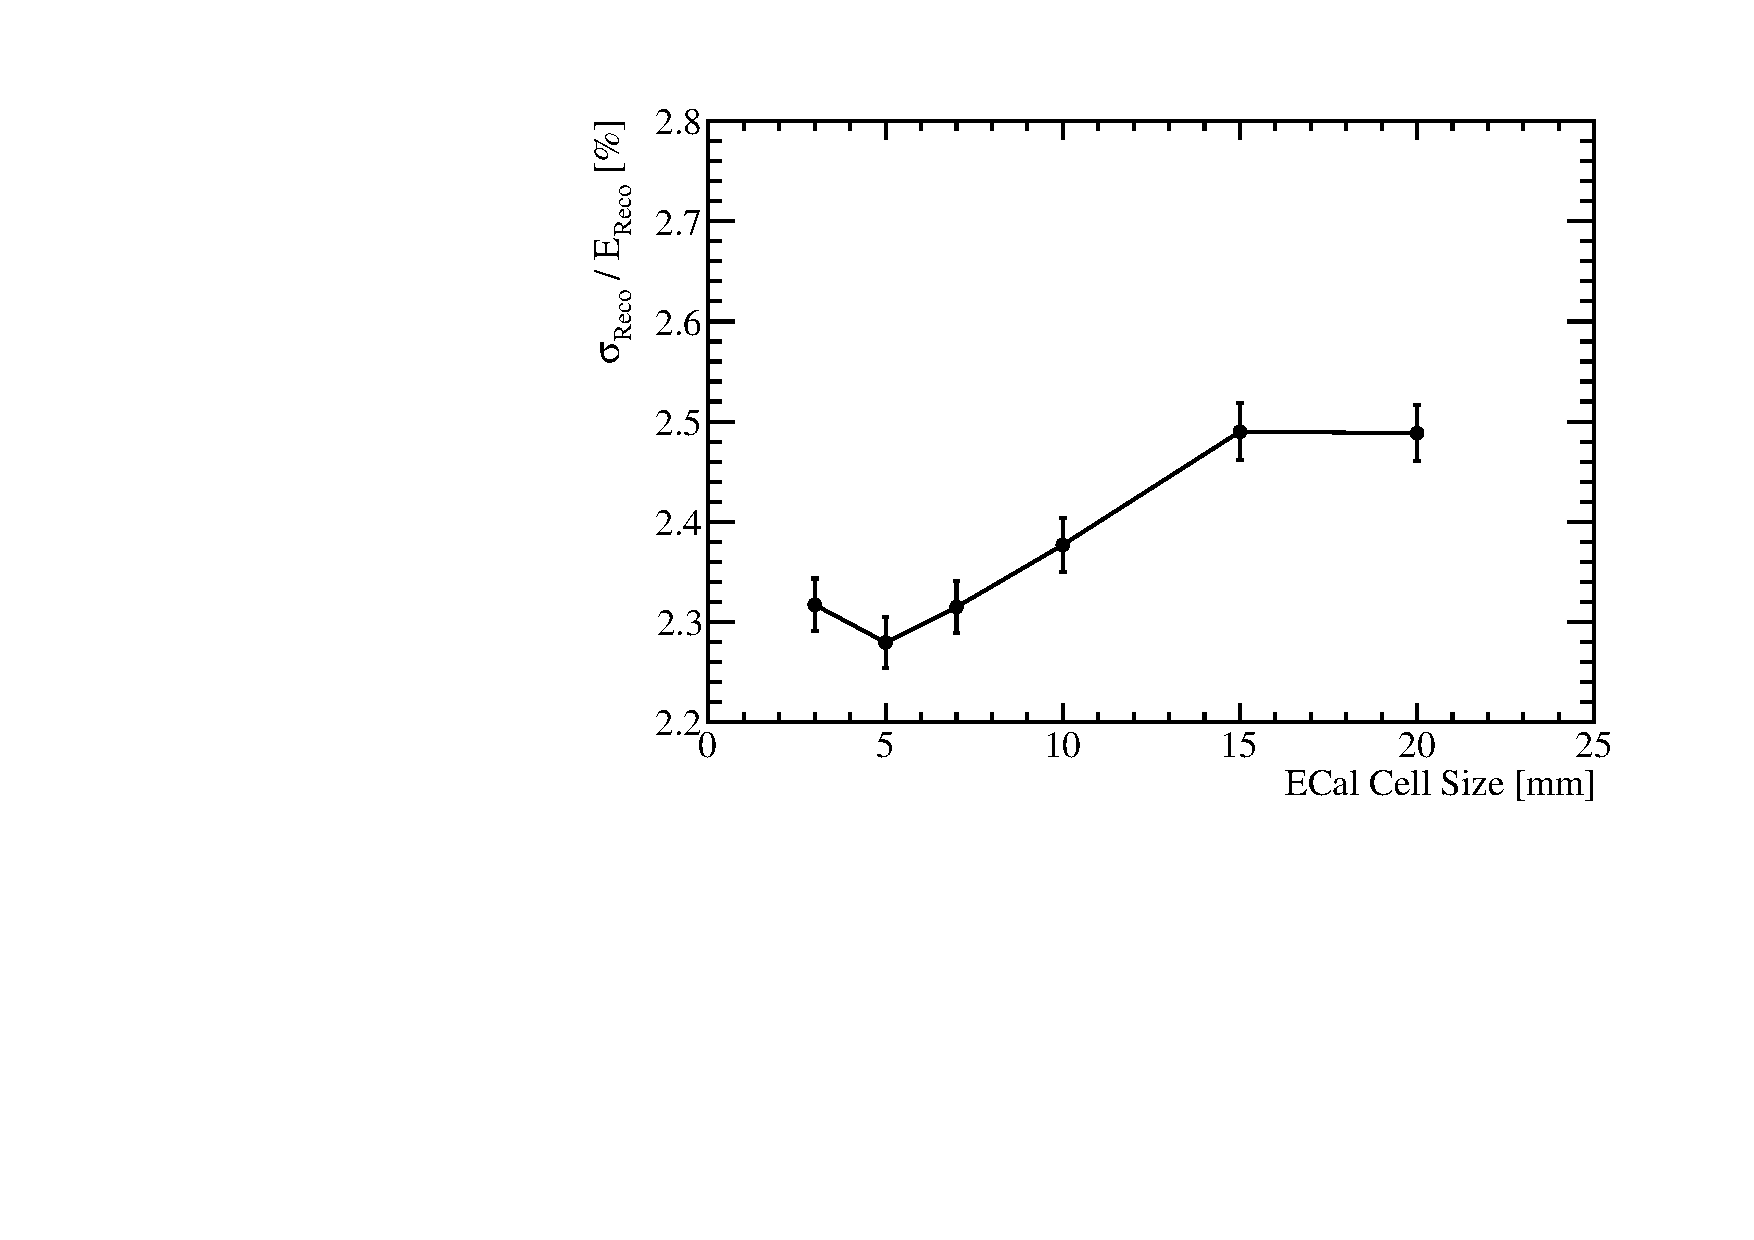
\includegraphics[width=0.5\textwidth]{OptimisationStudies/Plots/EnergyResolution/ER_vs_SiECalCellSize_100GeVPhoton.pdf}}
\subfloat[]{\label{fig:ecalsccellsize100gamma}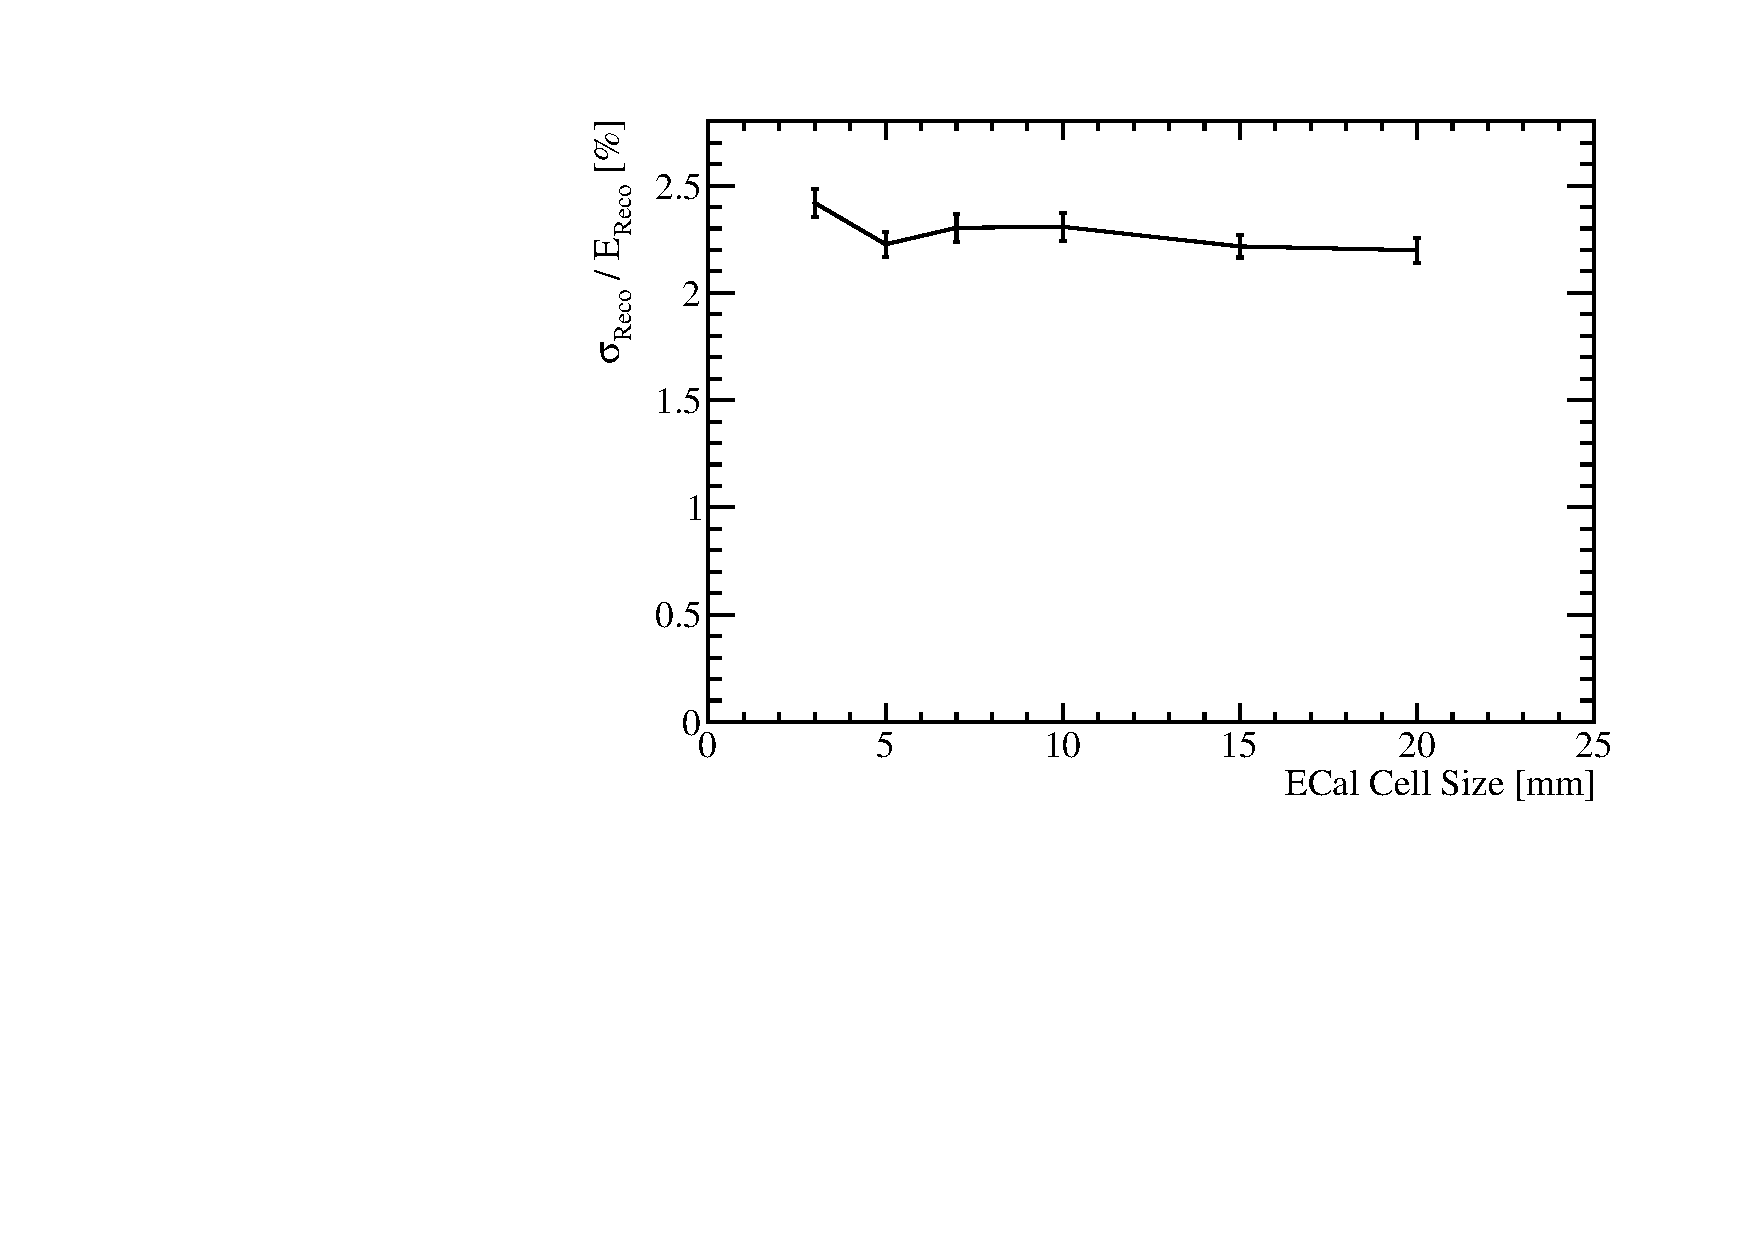
\includegraphics[width=0.5\textwidth]{OptimisationStudies/Plots/EnergyResolution/ER_vs_ScECalCellSize_100GeVPhoton.pdf}}
\caption[The energy resolution as a function of ECal cell size for 100~GeV $\gamma$s using the nominal ILD detector model with \protect\subref{fig:ecalsicellsize100gamma} the silicon and \protect\subref{fig:ecalsccellsize100gamma} the scintillator ECal option.]{The energy resolution as a function of ECal cell size for 100~GeV $\gamma$s using the nominal ILD detector model with \protect\subref{fig:ecalsicellsize100gamma} the silicon and \protect\subref{fig:ecalsccellsize100gamma} the scintillator ECal option.}
\label{fig:ecalcellsizegamma}
\end{figure}

The separation of nearby particle showers within the calorimeter is fundamentally limited by the cell size.  The smaller the cell size the easier it is to separate nearby particle showers and the better this separation the smaller the affect from confusion is.  Therefore, it is expected that the jet energy resolution be sensitive to the ECal cell size even though the intrinsic energy resolution is not.  The jet energy resolution as a function of ECal cell size is shown in figure \ref{fig:ecalsicellsize} for the silicon option and figure \ref{fig:ecalsccellsize} for the scintillator option.  As expected there is a very strong dependancy on the ECal cell size, with smaller cell sizes leading to lower values of the jet energy resolution.  The origin of this trend is best illustrated by considering the intrinsic energy resolution and confusion contributions to the jet energy resolution.  These contributions are shown as a function of ECal cell size for 45 and 250~GeV jets, for both the silicon and scintillator ECal options, in figure \ref{fig:ecalcellsizebreak}.  It is clear from these contributions that the intrinsic energy resolution of the detector does not change when varying the cell size, which agrees with both prior expectations of calorimeter behaviour and the single particle energy resolution study.  The minor fluctuations seen in the energy resolution for the single particle study are washed out when considering the intrinsic energy resolution for jets, as only $~30\%$ of jet energy is carried in the form of $\gamma$s.  Furthermore, it can be seen that the trend in jet energy resolution as a function of the ECal cell size is being driven purely by changes to the confusion contribution and, in particular, the confusion caused by the reconstruction of $\gamma$s.  This is exactly what is to expected given the ECal primarily measures $\gamma$s and shows that the performance of the ECal when varying the cell size is well understood.

\begin{figure}[h!]
\centering
\subfloat[]{\label{fig:ecalsicellsize}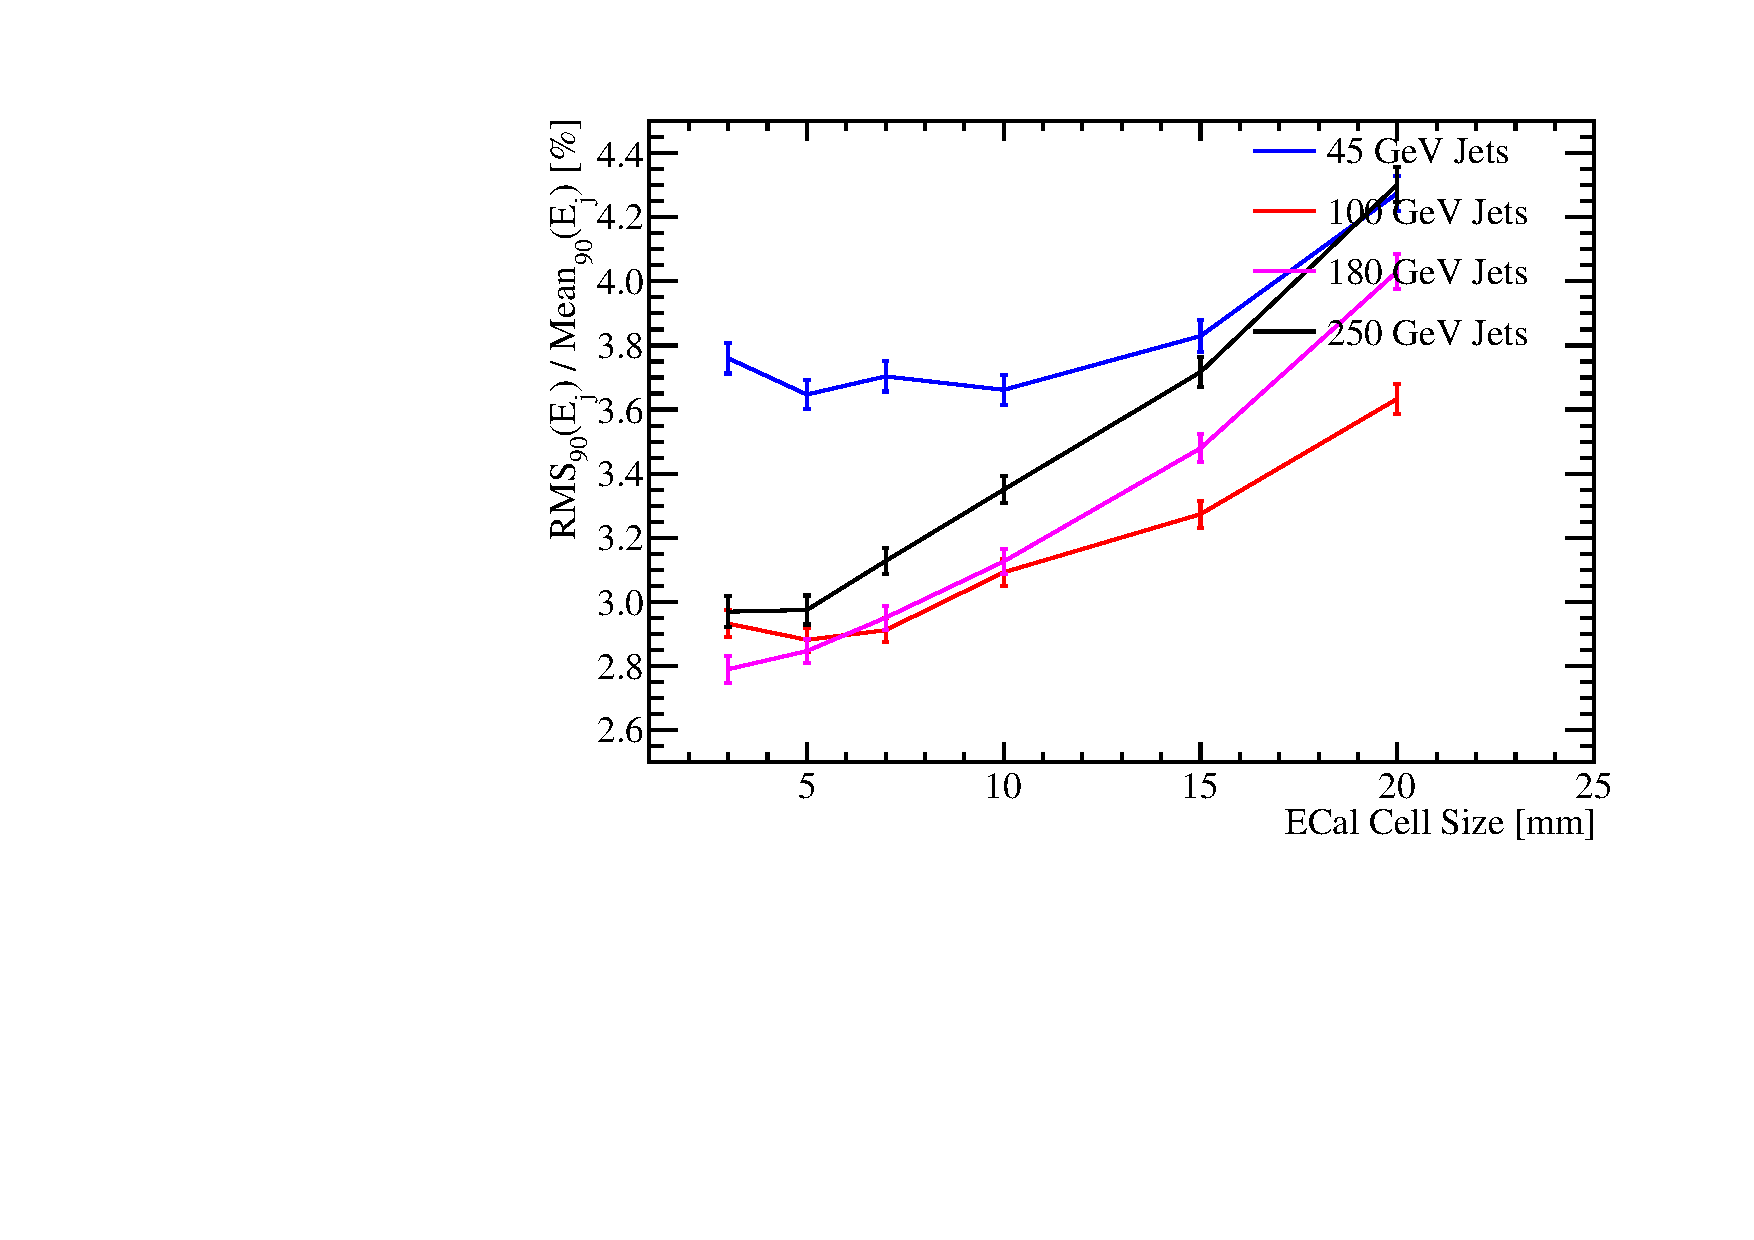
\includegraphics[width=0.5\textwidth]{OptimisationStudies/Plots/JetEnergyResolutions/JER_vs_SiliconECalCellSize.pdf}}
\subfloat[]{\label{fig:ecalsccellsize}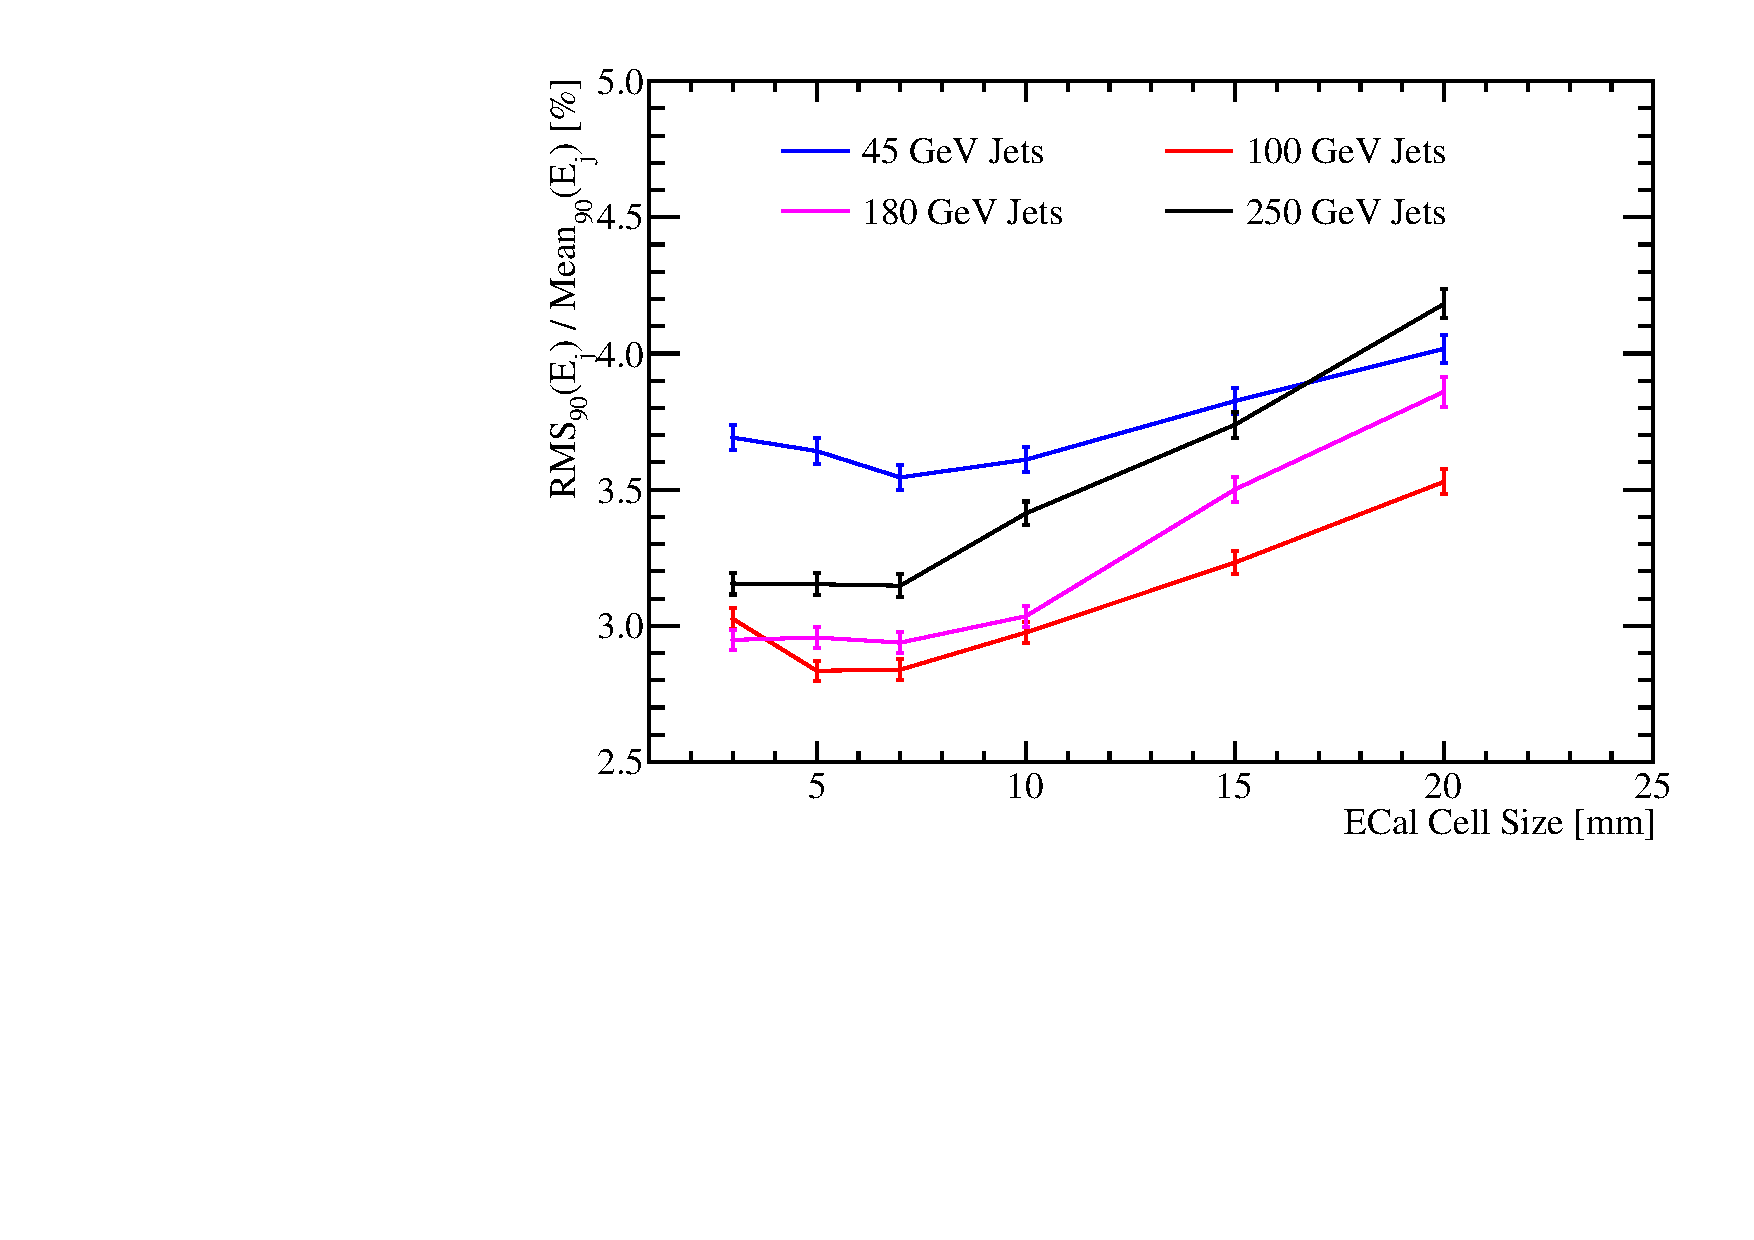
\includegraphics[width=0.5\textwidth]{OptimisationStudies/Plots/JetEnergyResolutions/JER_vs_ScintillatorECalCellSize.pdf}} \hfill
\caption[The jet energy resolution as a function of ECal cell size for various jet energies using the nominal ILD detector model with \protect\subref{fig:ecalsicellsize} the silicon and \protect\subref{fig:ecalsccellsize} the scintillator ECal option.]{The jet energy resolution as a function of ECal cell size for various jet energies using the nominal ILD detector model with \protect\subref{fig:ecalsicellsize} the silicon and \protect\subref{fig:ecalsccellsize} the scintillator ECal option.}
\label{fig:ecalcellsize}
\end{figure}

\begin{figure}[h!]
\centering
\subfloat[]{\label{fig:ecalsicellsize45break}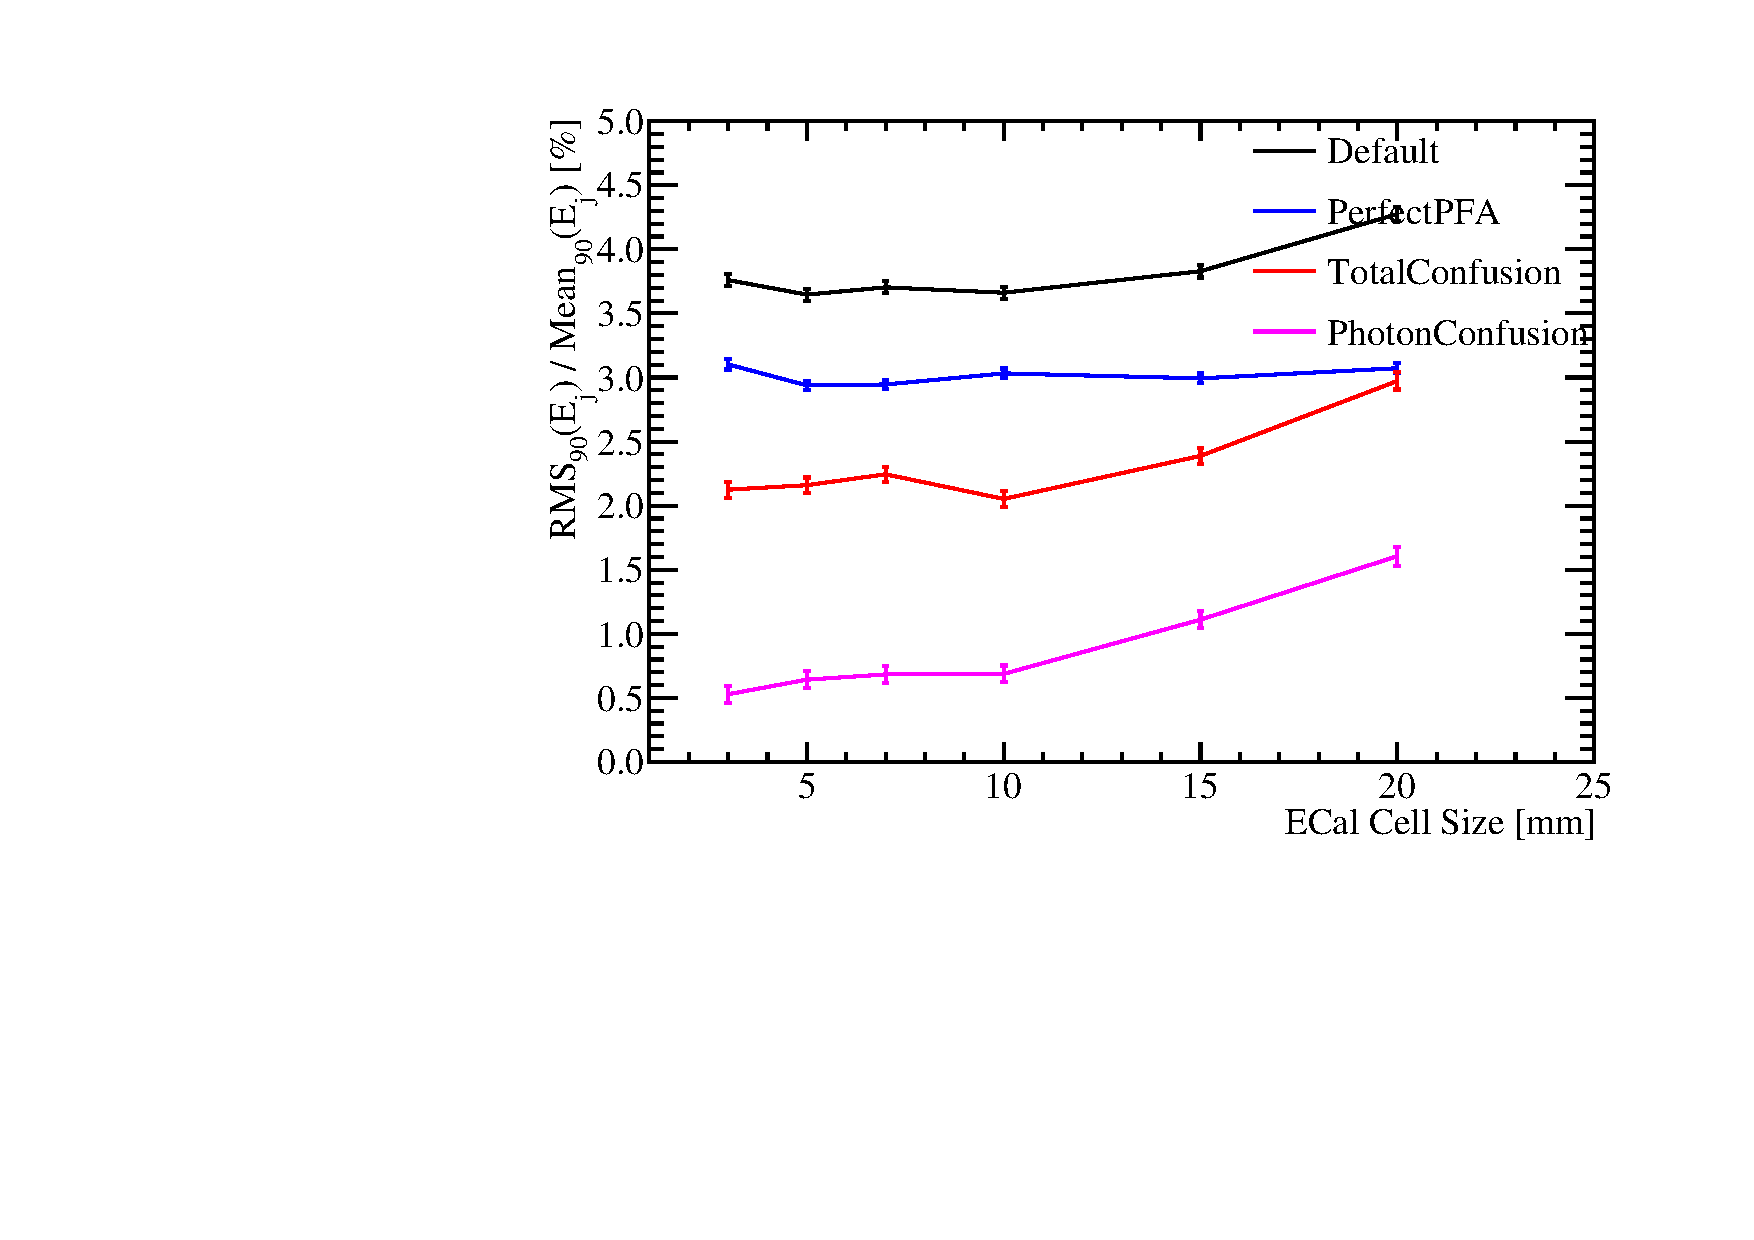
\includegraphics[width=0.5\textwidth]{OptimisationStudies/Plots/JetEnergyResolutions/JER_vs_SiliconECalCellSize_91GeV_DiJet_Breakdown.pdf}}
\subfloat[]{\label{fig:ecalsccellsize45break}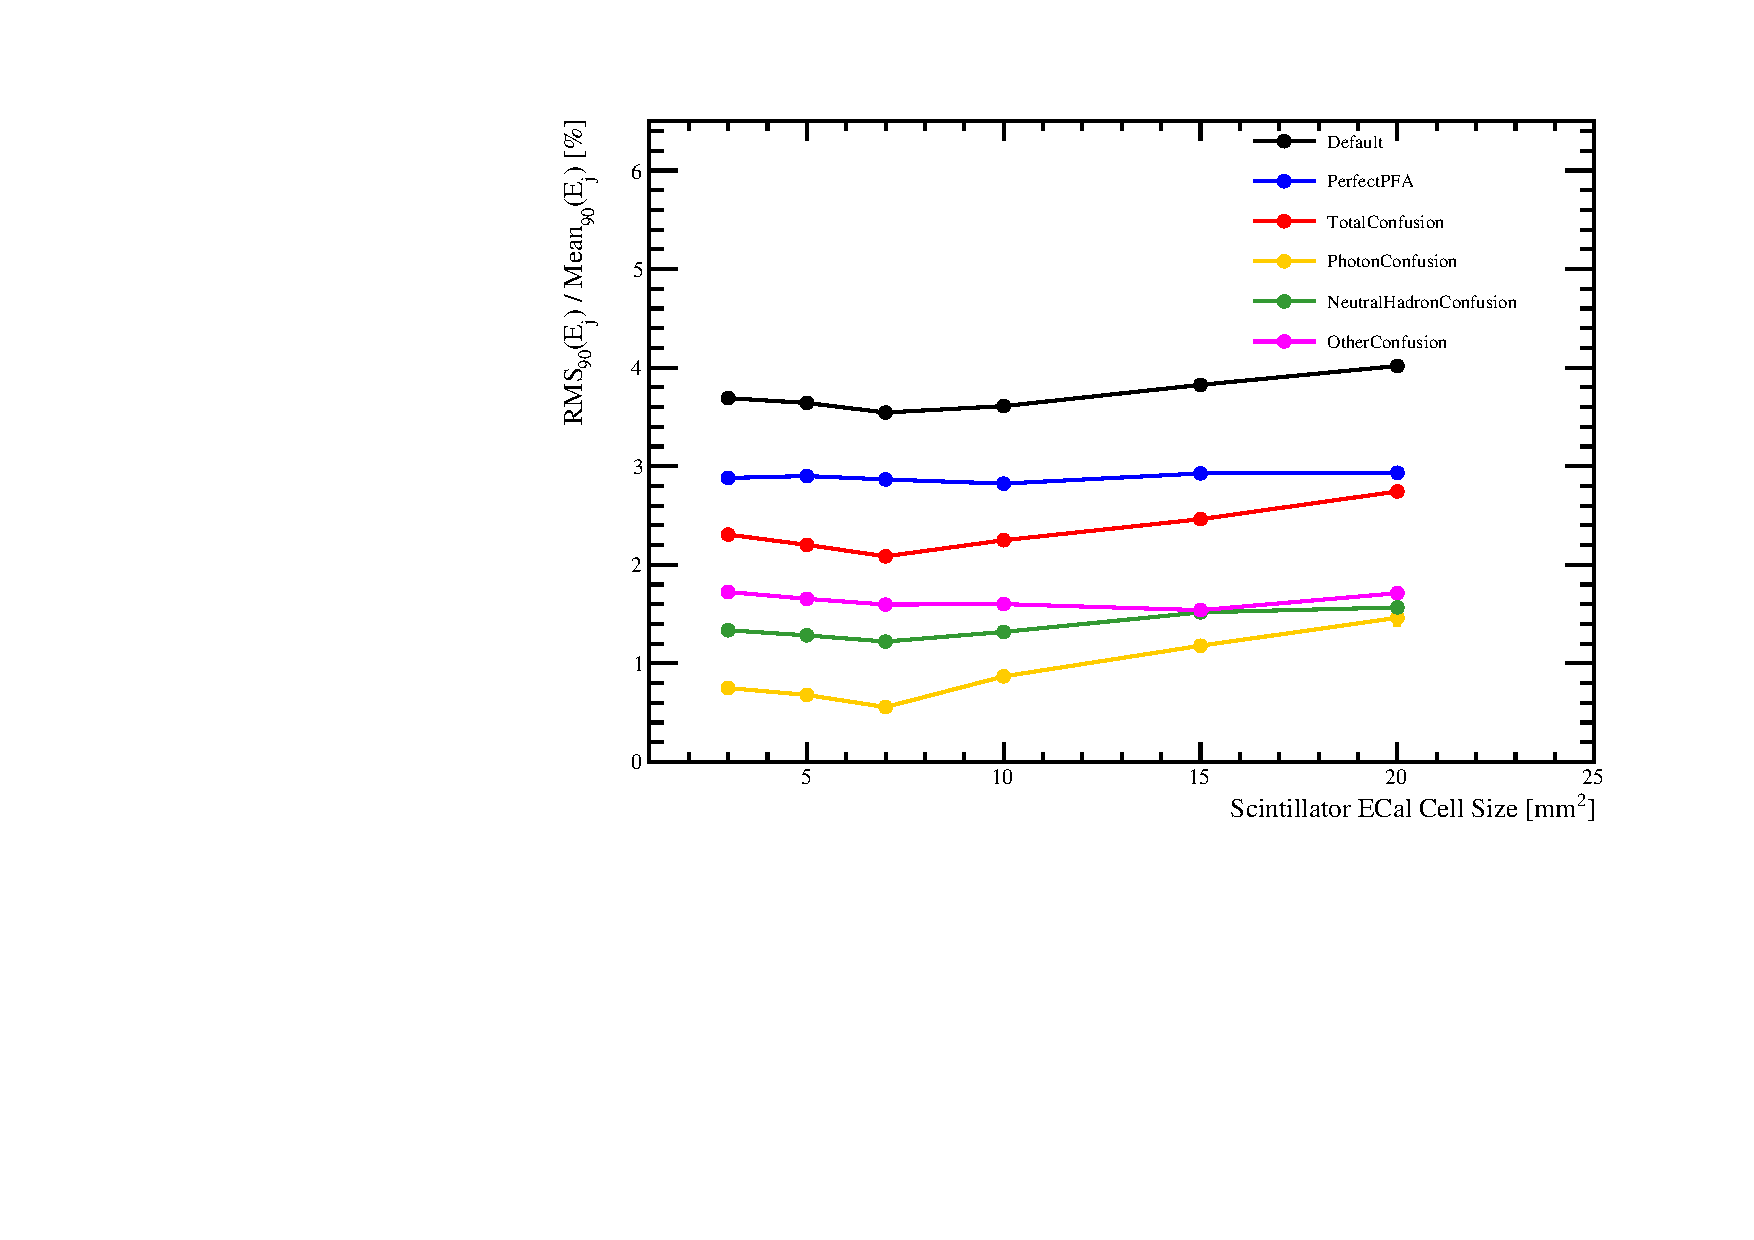
\includegraphics[width=0.5\textwidth]{OptimisationStudies/Plots/JetEnergyResolutions/JER_vs_ScintillatorECalCellSize_91GeV_DiJet_Breakdown.pdf}} \hfill
\subfloat[]{\label{fig:ecalsicellsize250break}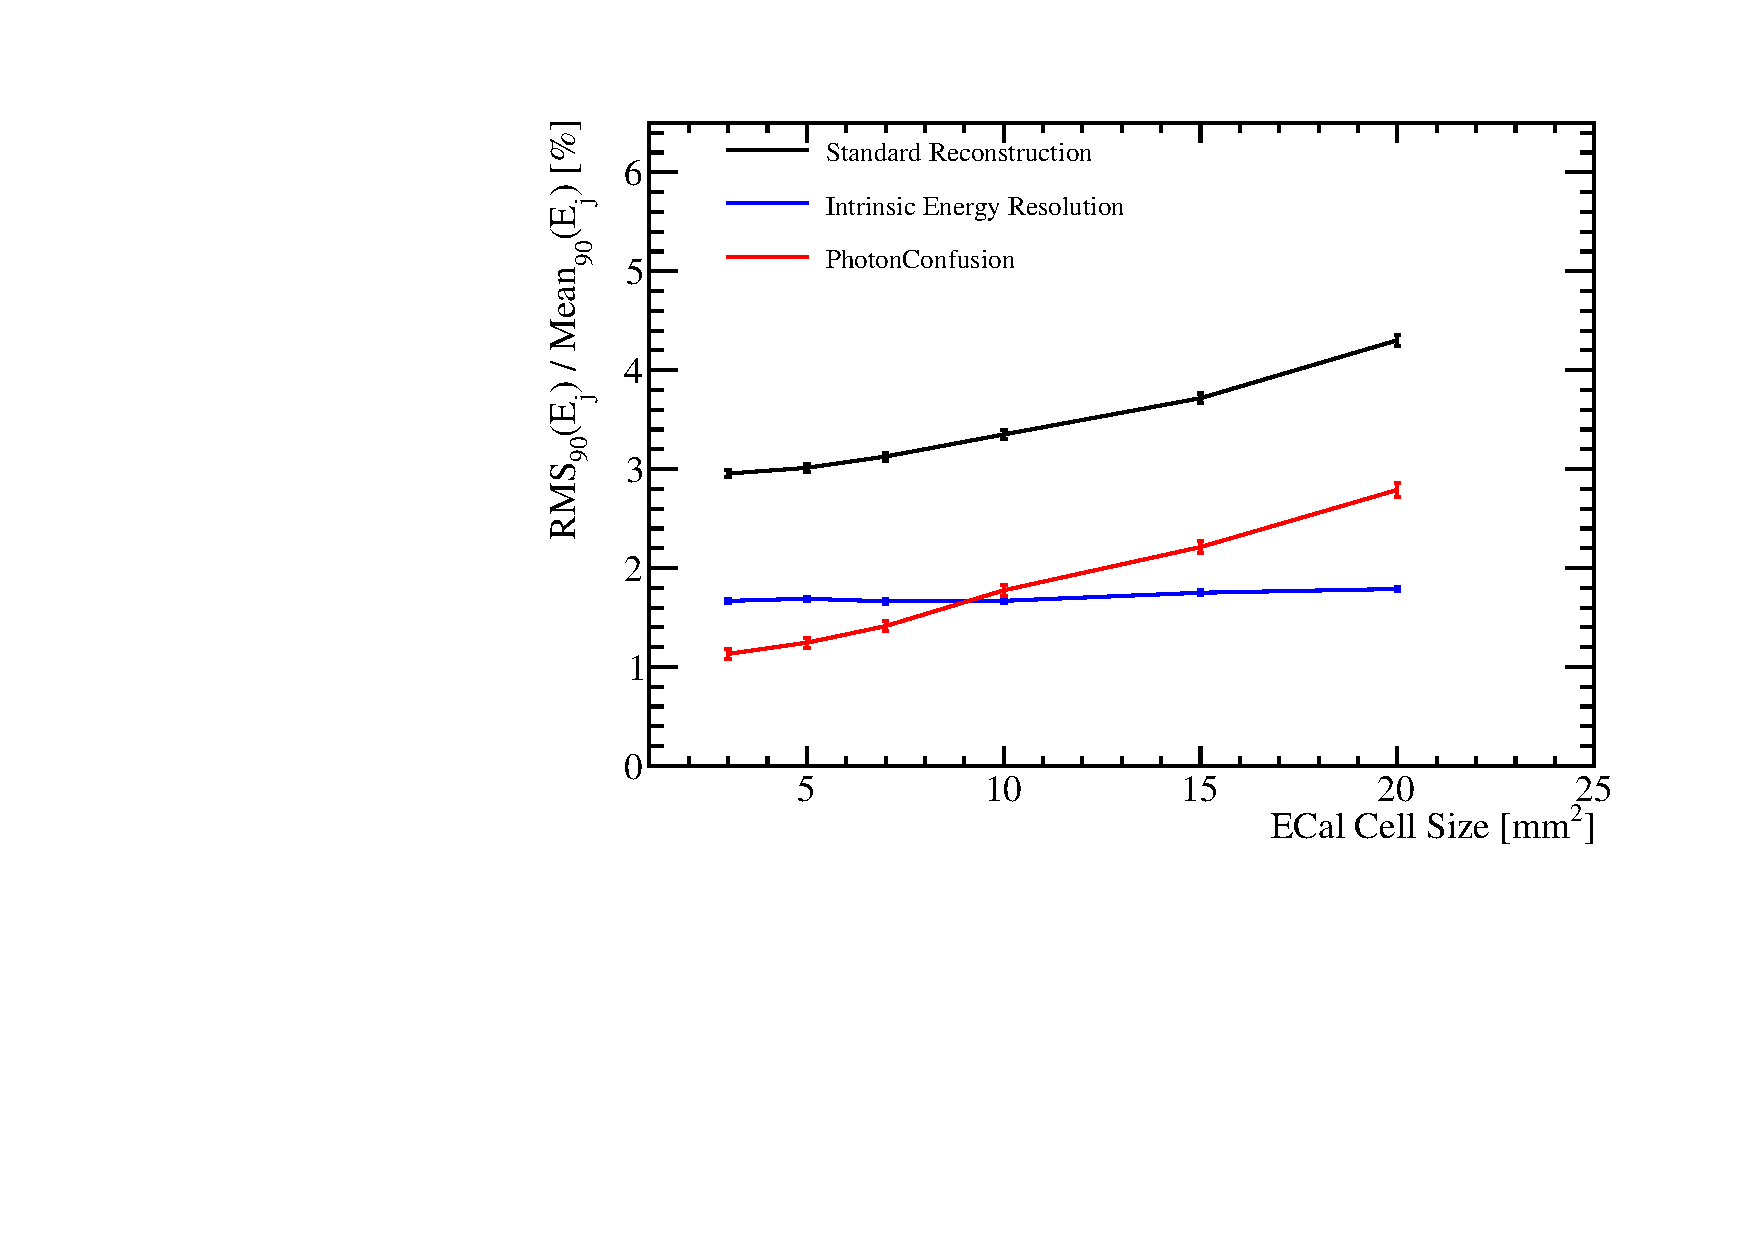
\includegraphics[width=0.5\textwidth]{OptimisationStudies/Plots/JetEnergyResolutions/JER_vs_SiliconECalCellSize_500GeV_DiJet_Breakdown.pdf}}
\subfloat[]{\label{fig:ecalsccellsize250break}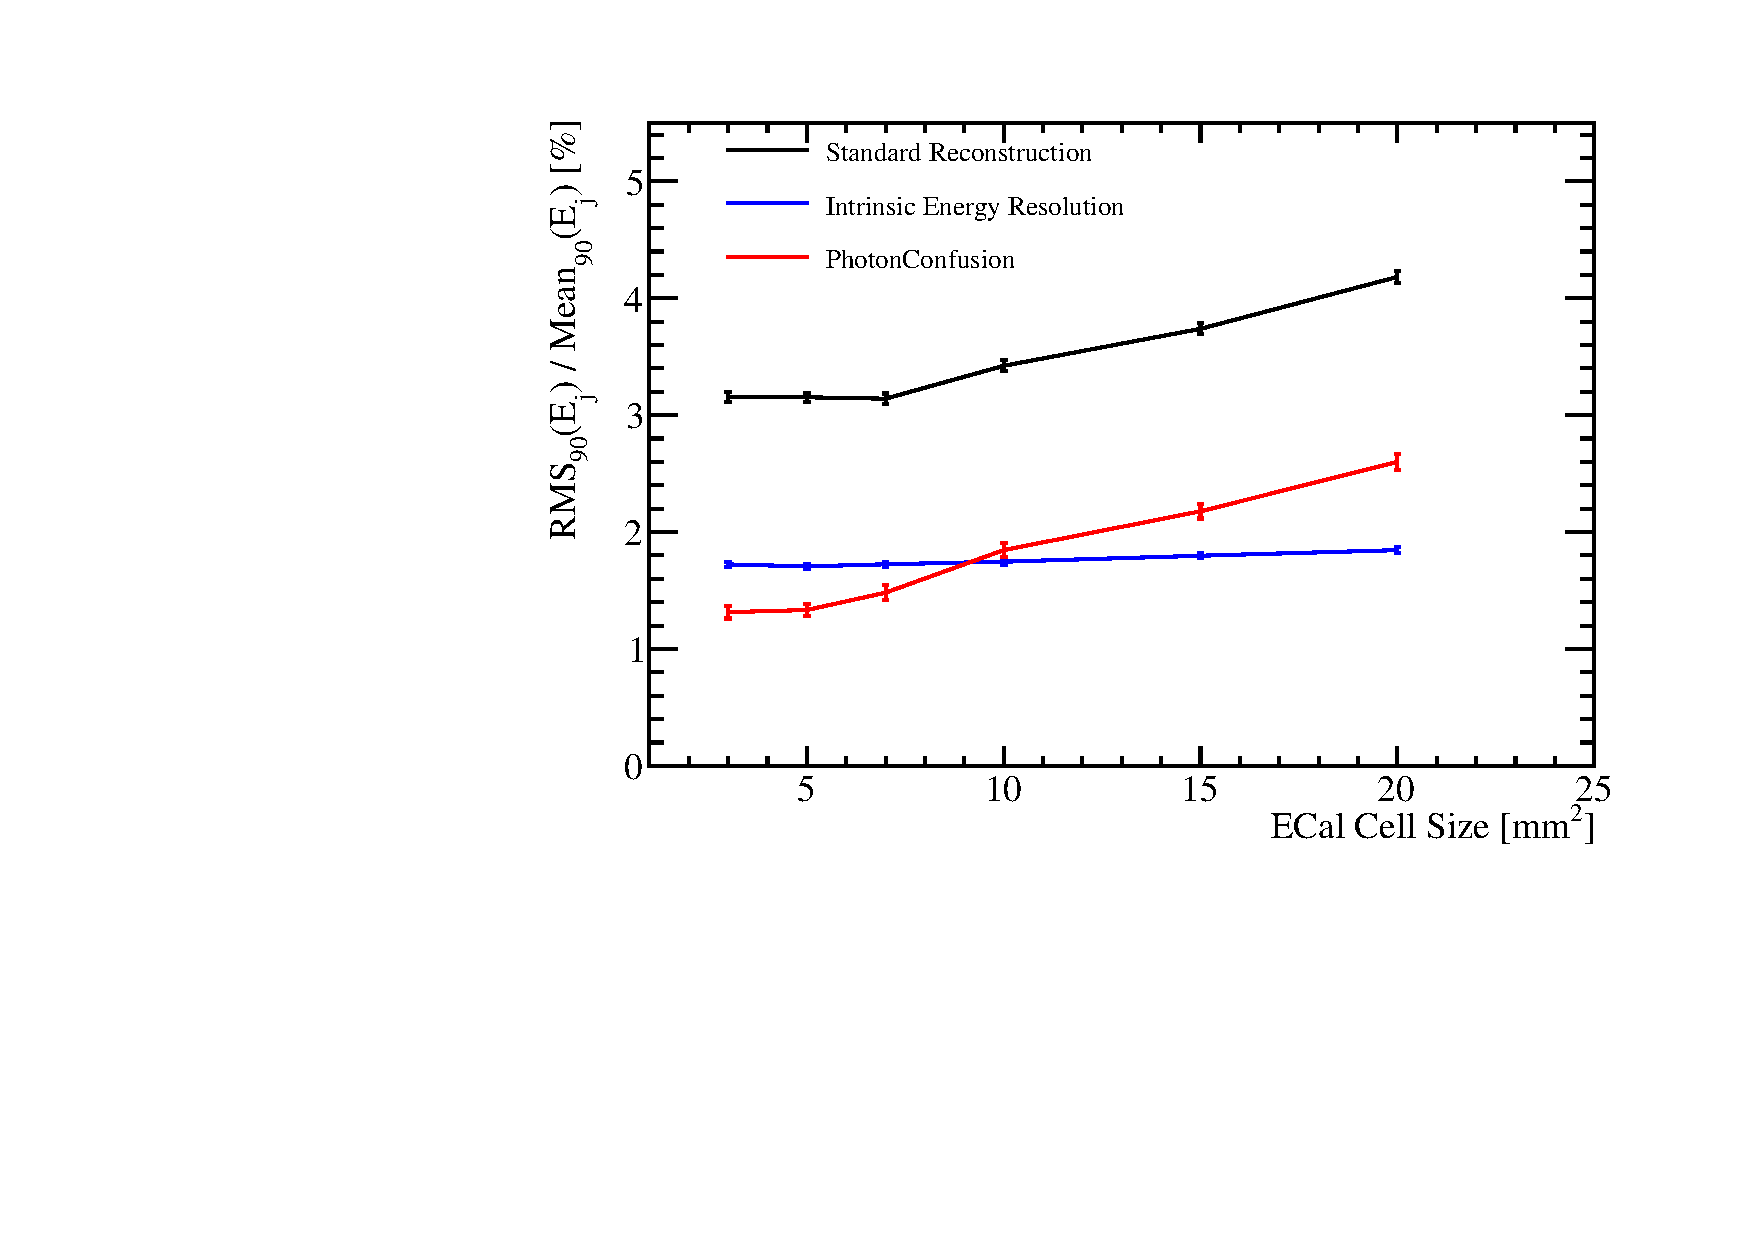
\includegraphics[width=0.5\textwidth]{OptimisationStudies/Plots/JetEnergyResolutions/JER_vs_ScintillatorECalCellSize_500GeV_DiJet_Breakdown.pdf}}
\caption[The contributions to the jet energy resolution as a function of ECal cell size using the nominal ILD detector model for \protect\subref{fig:ecalsicellsize45break} the silicon ECal option and 45~GeV jets, \protect\subref{fig:ecalsccellsize45break} the scintillator ECal option and 45~GeV jets, \protect\subref{fig:ecalsicellsize250break} the silicon ECal option and 250~GeV jets and \protect\subref{fig:ecalsccellsize250break} the scintillator ECal option and 250~GeV jets.  The black curves correspond to the standard reconstruction, the blue curves to the intrinsic energy resolution contribution to the jet energy resolution, the red curves to the confusion contribution to the jet energy resolution and the magenta curves to the confusion contribution to the jet energy resolution related solely to $\gamma$ reconstruction.]{The contributions to the jet energy resolution as a function of ECal cell size using the nominal ILD detector model for \protect\subref{fig:ecalsicellsize45break} the silicon ECal option and 45~GeV jets, \protect\subref{fig:ecalsccellsize45break} the scintillator ECal option and 45~GeV jets, \protect\subref{fig:ecalsicellsize250break} the silicon ECal option and 250~GeV jets and \protect\subref{fig:ecalsccellsize250break} the scintillator ECal option and 250~GeV jets.  The black curves correspond to the standard reconstruction, the blue curves to the intrinsic energy resolution contribution to the jet energy resolution, the red curves to the confusion contribution to the jet energy resolution and the magenta curves to the confusion contribution to the jet energy resolution related solely to $\gamma$ reconstruction}
\label{fig:ecalcellsizebreak}
\end{figure}

It is clear that the ECal cell size is extremely important for jet energy measurements, although it has little bearing on the intrinsic energy resolution of the ECal.  To ensure separation of hadronic decays of W and Z bosons is possible at ILC like energies, an ECal cell size of least $15 \times 15 \text{mm}^{2}$ is crucial.  However, as reducing the ECal cell size beyond this leads to further improves the jet energy resolution choosing the smallest ECal cell size is desirable.

%========================================================================================

\subsection{ECal Sampling Frequency} 
\label{sec:ecalnlayers}
The detector performance was simulated where the number of layers in the ECal was varied, while keeping the total material budget ($\text{X}_{0}$) approximately constant.  This study was performed for both the silicon and scintillator active material options.  In all cases tungsten was used for the ECal absorber material and the active layer thicknesses were not changed from those used in the nominal ILD ECal summarised in table \ref{table:defaultildecal}.  The different layouts for the ECals considered here are summarised in table \ref{table:nlayersecaloption}.  

\begin{table}[h!]
\centering
\begin{tabular}{ r r r r r r}
\hline
Total Number & $N_{Layers}$ & Absorber & $N_{Layers}$ & Absorber & Total  \\
of Layers & Region 1 & Thickness & Region 2 & Thickness & Thickness \\
$N_{\text{Layers ECal}}$ & & Region 1 [mm] & &  Region 2 [mm] &  [$\text{X}_{0}$] \\
\hline
30 & 20 & 2.10 & 9 & 4.20 & 22.77 \\
26 & 17 & 2.40 & 8 & 4.80 & 22.60 \\
20 & 13 & 3.15 & 6 & 6.30 & 22.47 \\
16 & 10 & 4.00 & 5 & 8.00 & 22.31\\
\hline
\end{tabular}
\caption[The longitudinal structure of the ECal models considered in the optimisation study.  The radiation length of tungsten absorber is 3.504mm \cite{Olive:2016xmw}.  Note that a presampler layer contributes one extra layer to the cumulative number of layers.]{The longitudinal structure of the ECal models considered in the optimisation study.  The radiation length of tungsten absorber is 3.504mm \cite{Olive:2016xmw}.  Note that a presampler layer contributes one extra layer to the cumulative number of layers.}
\label{table:nlayersecaloption}
\end{table}

The energy resolution, for 100~GeV $\gamma$ events, as a function of the number of layers in the ECal is shown in figure \ref{fig:ecalsinlayers100gamma} for the silicon option and in figure \ref{fig:ecalscnlayers100gamma} for the scintillator option.  As the number of layers is reduced the energy resolution increases, which is expected as more layers leads to greater sampling of the particle shower and a reduction in the stochastic contribution to the energy resolution.  

\begin{figure}[h!]
\centering
\subfloat[]{\label{fig:ecalsinlayers100gamma}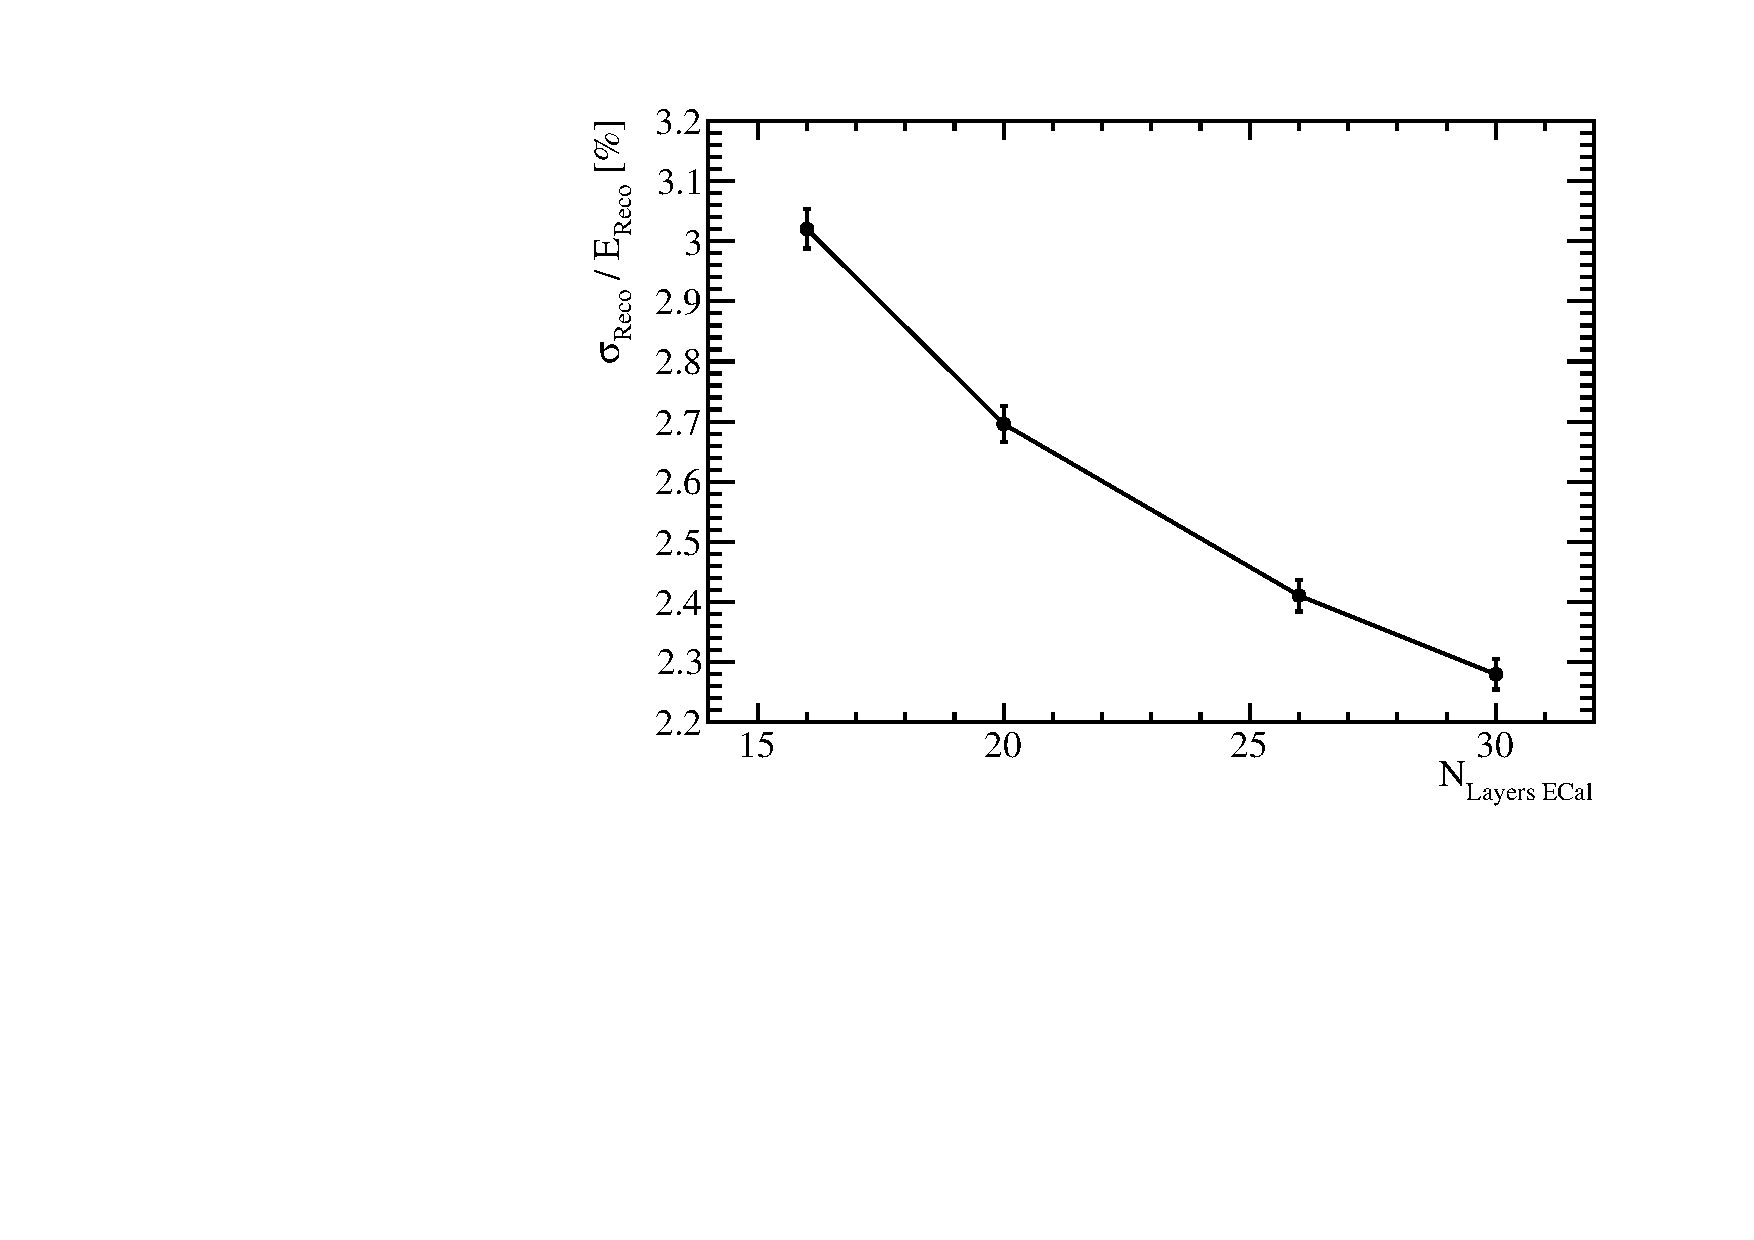
\includegraphics[width=0.5\textwidth]{OptimisationStudies/Plots/EnergyResolution/ER_vs_SiECalNLayers_100GeVPhoton.pdf}}
\subfloat[]{\label{fig:ecalscnlayers100gamma}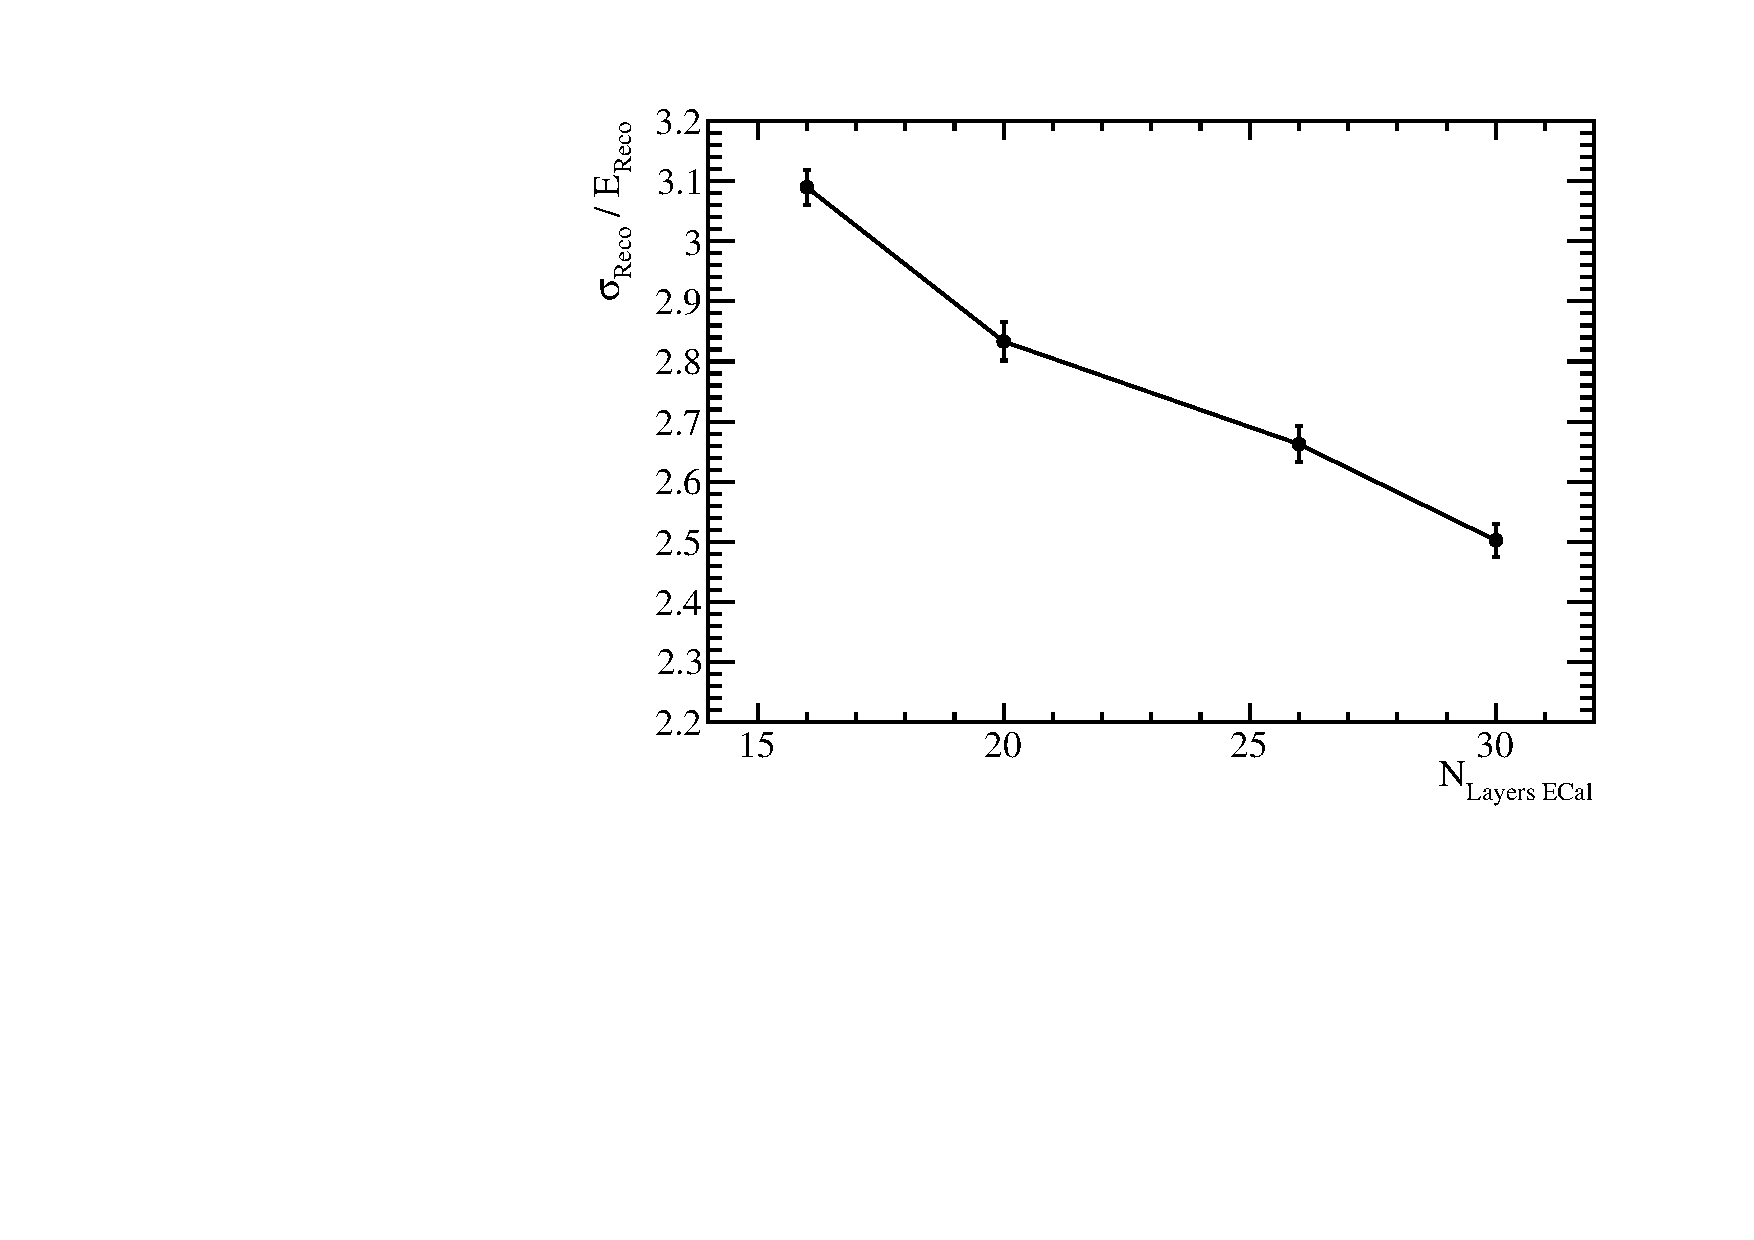
\includegraphics[width=0.5\textwidth]{OptimisationStudies/Plots/EnergyResolution/ER_vs_ScECalNLayers_100GeVPhoton.pdf}}
\caption[The energy resolution as a function of number of layers in the ECal for 100~GeV $\gamma$s using the nominal ILD detector model with \protect\subref{fig:ecalsinlayers100gamma} the silicon and \protect\subref{fig:ecalscnlayers100gamma} the scintillator ECal option.]{The energy resolution as a function of number of layers in the ECal for 100~GeV $\gamma$s using the nominal ILD detector model with \protect\subref{fig:ecalsinlayers100gamma} the silicon and \protect\subref{fig:ecalscnlayers100gamma} the scintillator ECal option.}
\label{fig:ecalnlayersgamma}
\end{figure}

When the number of layers in the ECal is increased, the intrinsic energy resolution of the ECal improves.  This has the knock-on effect of reducing the confusion contribution to the jet energy resolution, which can be seen in figures \ref{fig:ecalsinlayers} and \ref{fig:ecalscnlayers} for the silicon and scintillator ECal options respectively.  In both cases the jet energy resolution was found to improve when the number of layers in the ECal was increased.  The magnitude of the change in jet energy resolution was dependent upon the jet energy, with a stronger dependancy being observed for low energy jets.  This is expected from the stochastic contribution to the energy resolution for a sampling calorimeter, which is $\propto \frac{1}{\sqrt{E \times N_{Layers}}}$ where $E$ is the reconstructed energy and $N_{Layers}$ is the number of layers in the calorimeter.  At high jet energies, the energy resolution in the ECal is small and changes to the stochastic term that occur when varying the number of layers are too fine to be resolved using jet energy resolution.  While at low jet energies the stochastic term is larger making it possible to resolve the changes to it when varying the number of layers in the ECal.  The jet energy resolution is less sensitive than the single $\gamma$ energy resolution to changes in the number of ECal layers as only $\approx 30\%$ of jet energy is carried in the form of $\gamma$s.  The decomposition of the jet energy resolution into the intrinsic energy resolution and confusion contributions for 45 and 250~GeV jets are shown, for both the silicon and scintillator ECal options, in figure \ref{fig:ecalnlayersbreak}.  

As expected, the improvement to the intrinsic energy resolution seen when increasing the number of layers in the ECal leads to the knock-on effect of lowering the confusion.  However, significantly the magnitude of the change to the intrinsic energy resolution and confusion contributions to the jet energy resolution when varying the number of layers in the ECal are comparable in size.  This shows that pattern recognition is as important for detector performance in the particle flow paradigm than intrinsic energy resolution.  

\begin{figure}[h!]
\centering
\subfloat[]{\label{fig:ecalsinlayers}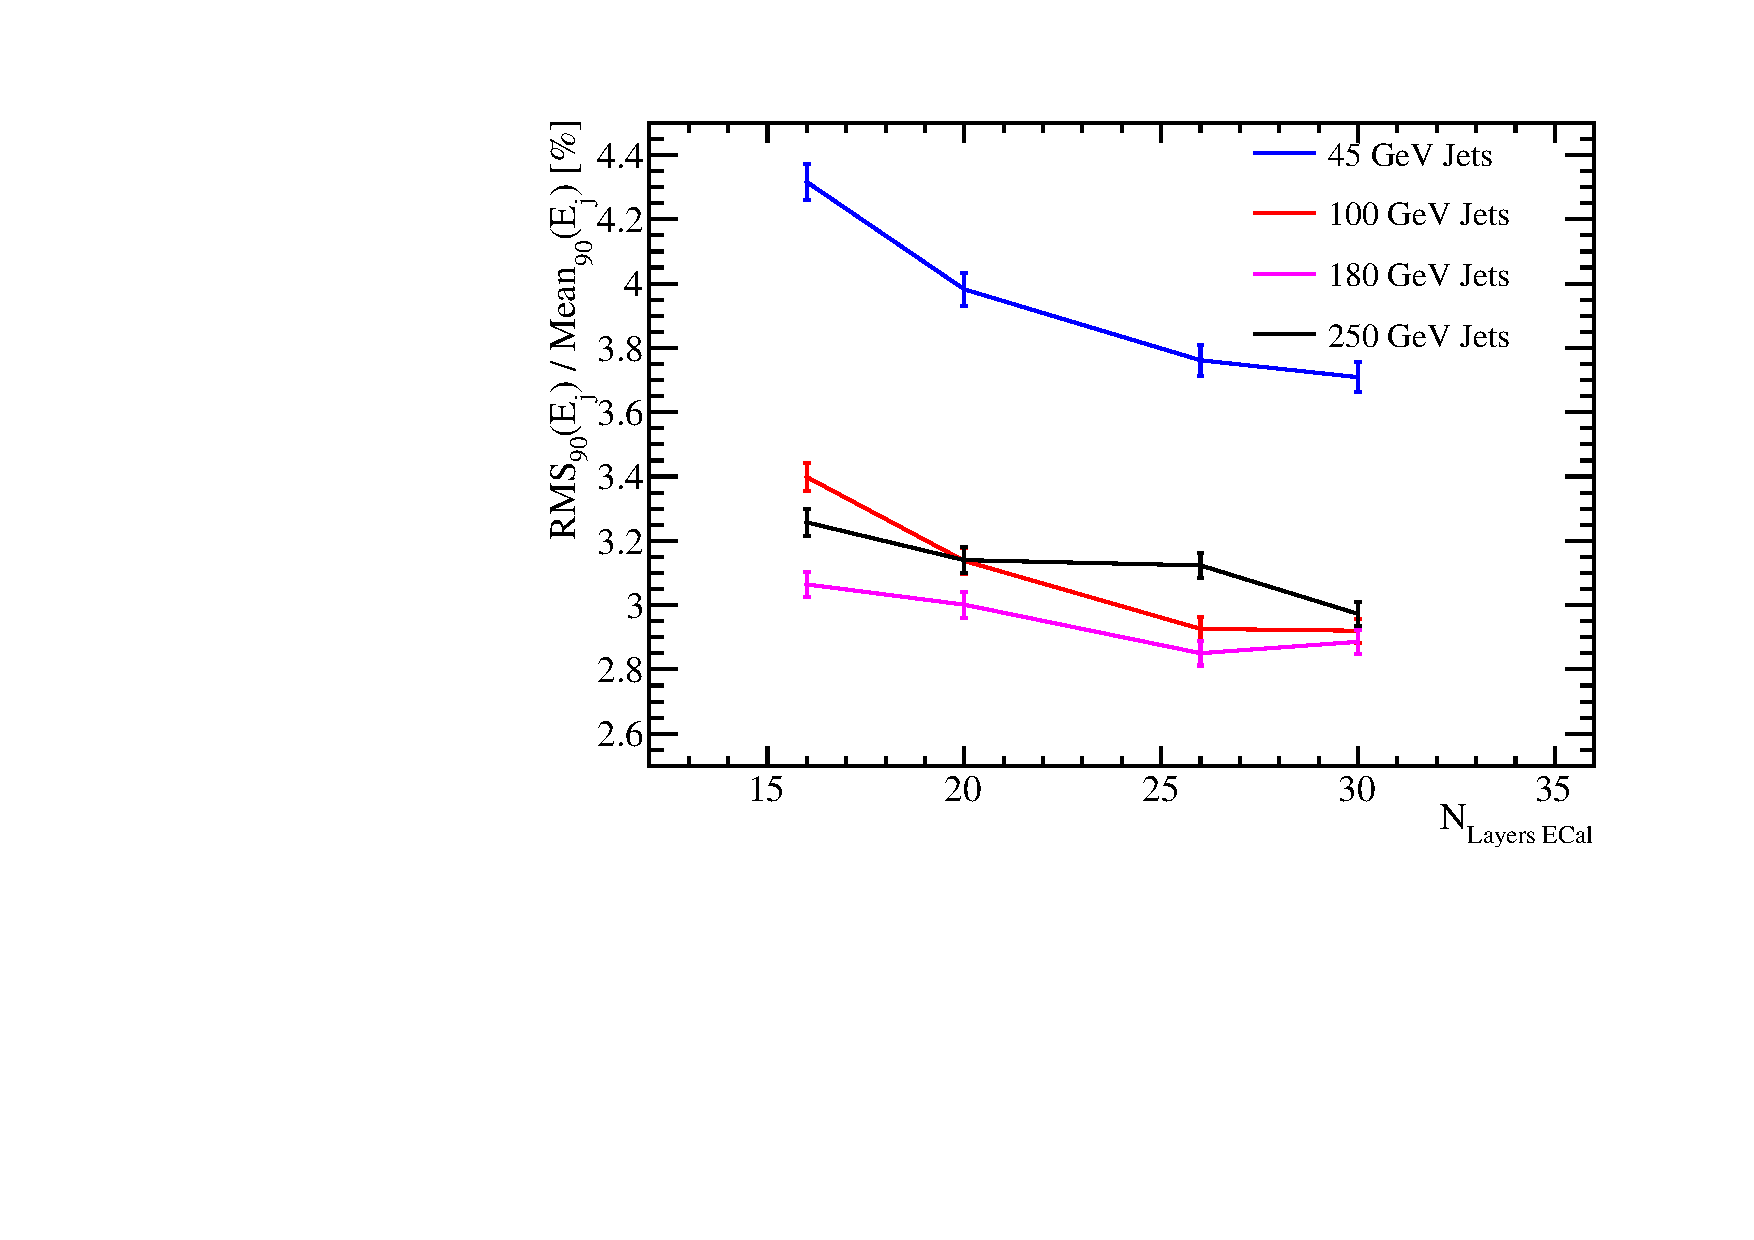
\includegraphics[width=0.5\textwidth]{OptimisationStudies/Plots/JetEnergyResolutions/JER_vs_SiliconECalNumberofLayers.pdf}}
\subfloat[]{\label{fig:ecalscnlayers}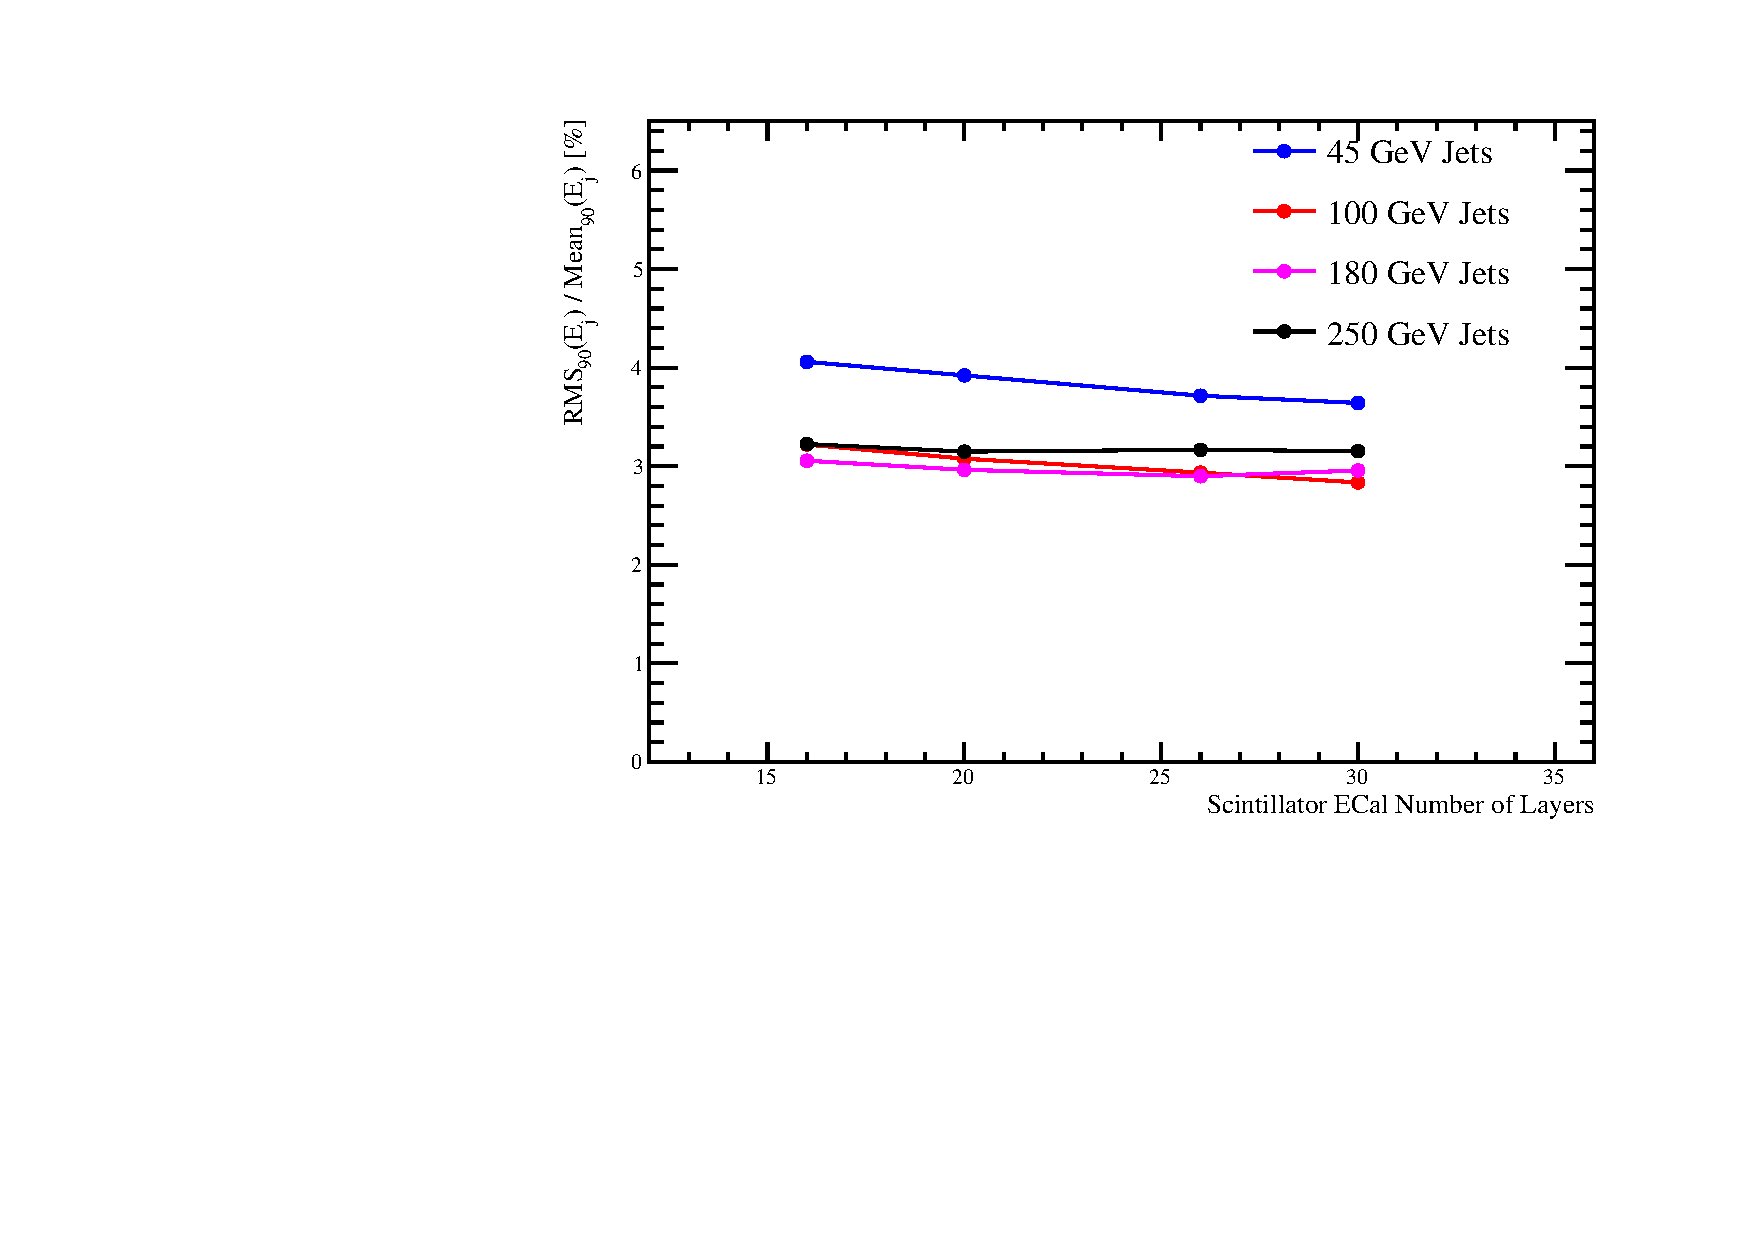
\includegraphics[width=0.5\textwidth]{OptimisationStudies/Plots/JetEnergyResolutions/JER_vs_ScintillatorECalNumberofLayers.pdf}} \hfill
\caption[The jet energy resolution as a function of number of layers in the ECal for various jet energies using the nominal ILD detector model with \protect\subref{fig:ecalsinlayers} the silicon and \protect\subref{fig:ecalscnlayers} the scintillator ECal option.]{The jet energy resolution as a function of number of layers in the ECal for various jet energies using the nominal ILD detector model with \protect\subref{fig:ecalsinlayers} the silicon and \protect\subref{fig:ecalscnlayers} the scintillator ECal option.}
\label{fig:ecalnlayers}
\end{figure}

\begin{figure}[h!]
\centering
\subfloat[]{\label{fig:ecalsinlayers45break}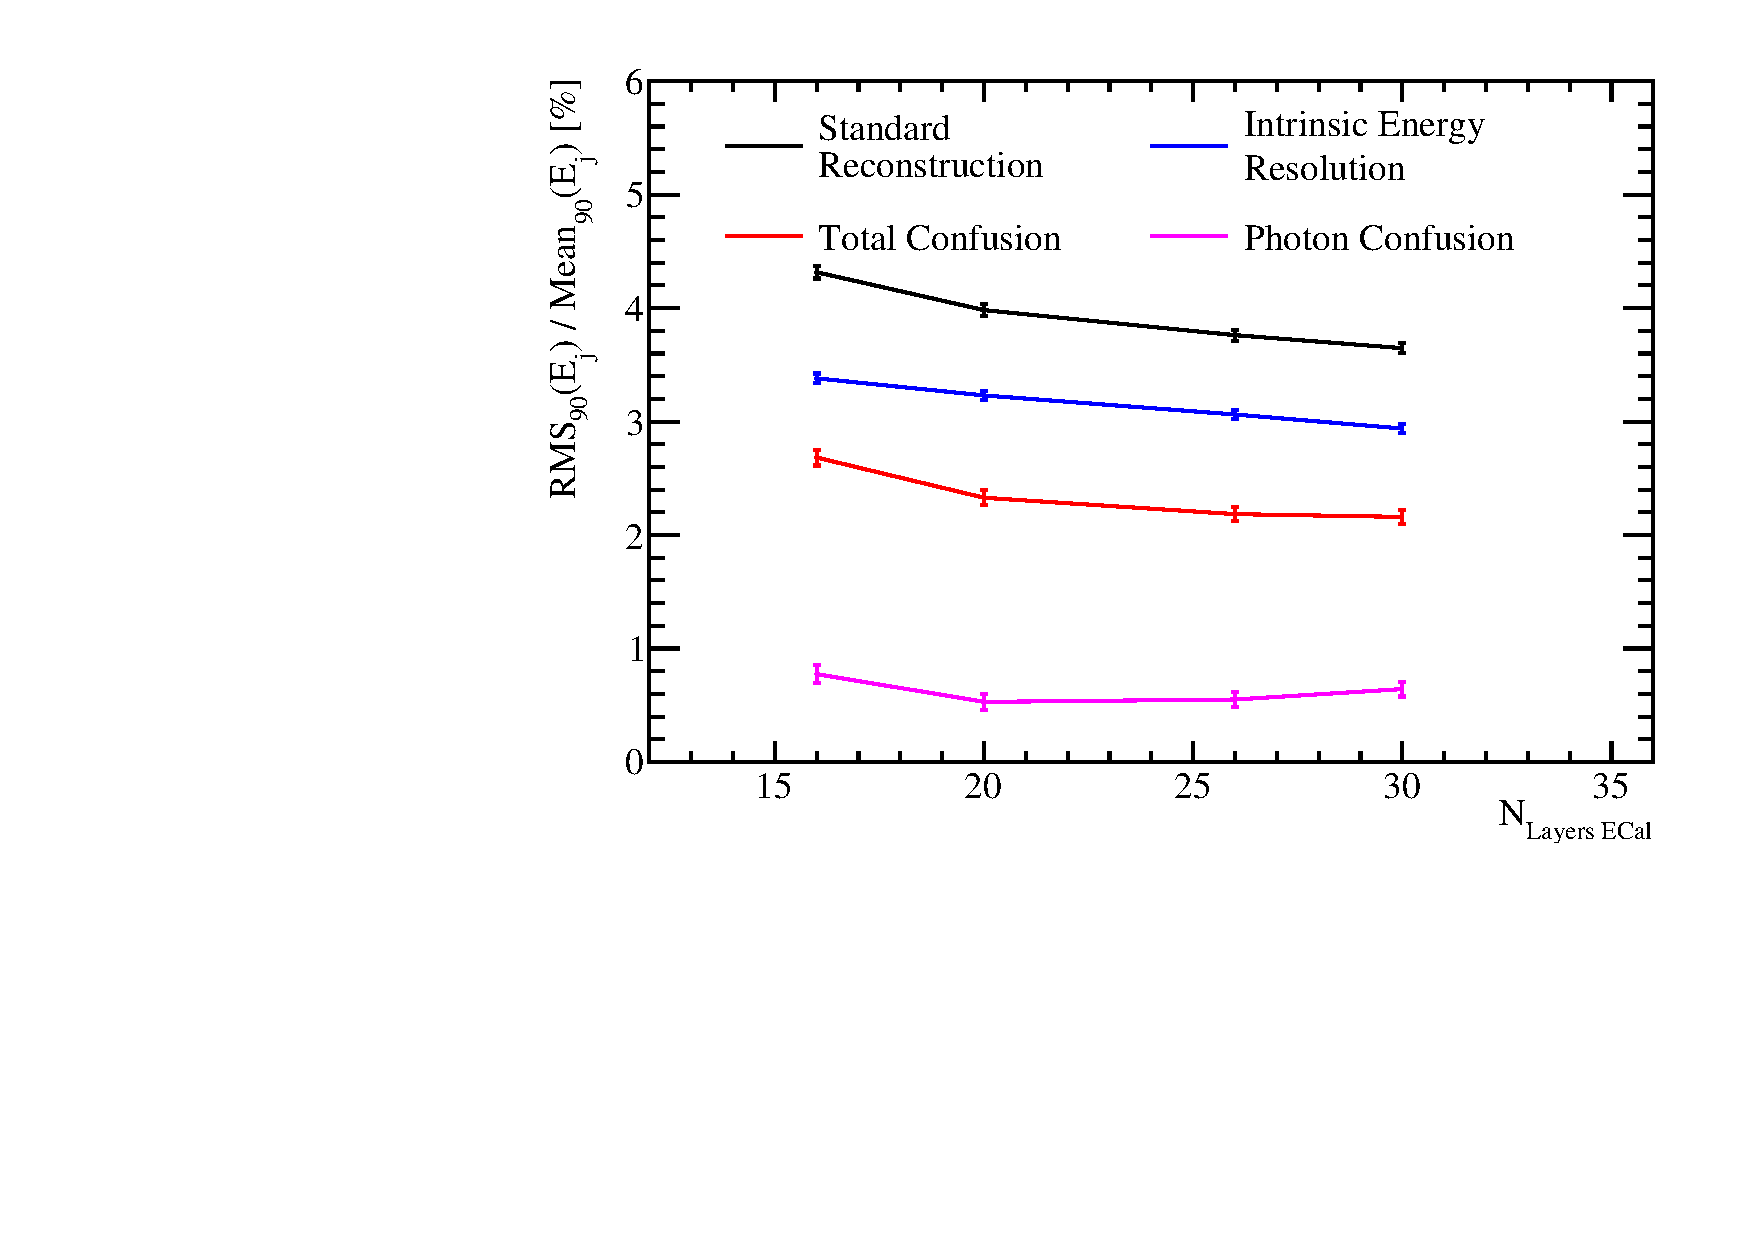
\includegraphics[width=0.5\textwidth]{OptimisationStudies/Plots/JetEnergyResolutions/JER_vs_SiliconECalNumberofLayers_91GeV_DiJet_Breakdown.pdf}}
\subfloat[]{\label{fig:ecalscnlayers45break}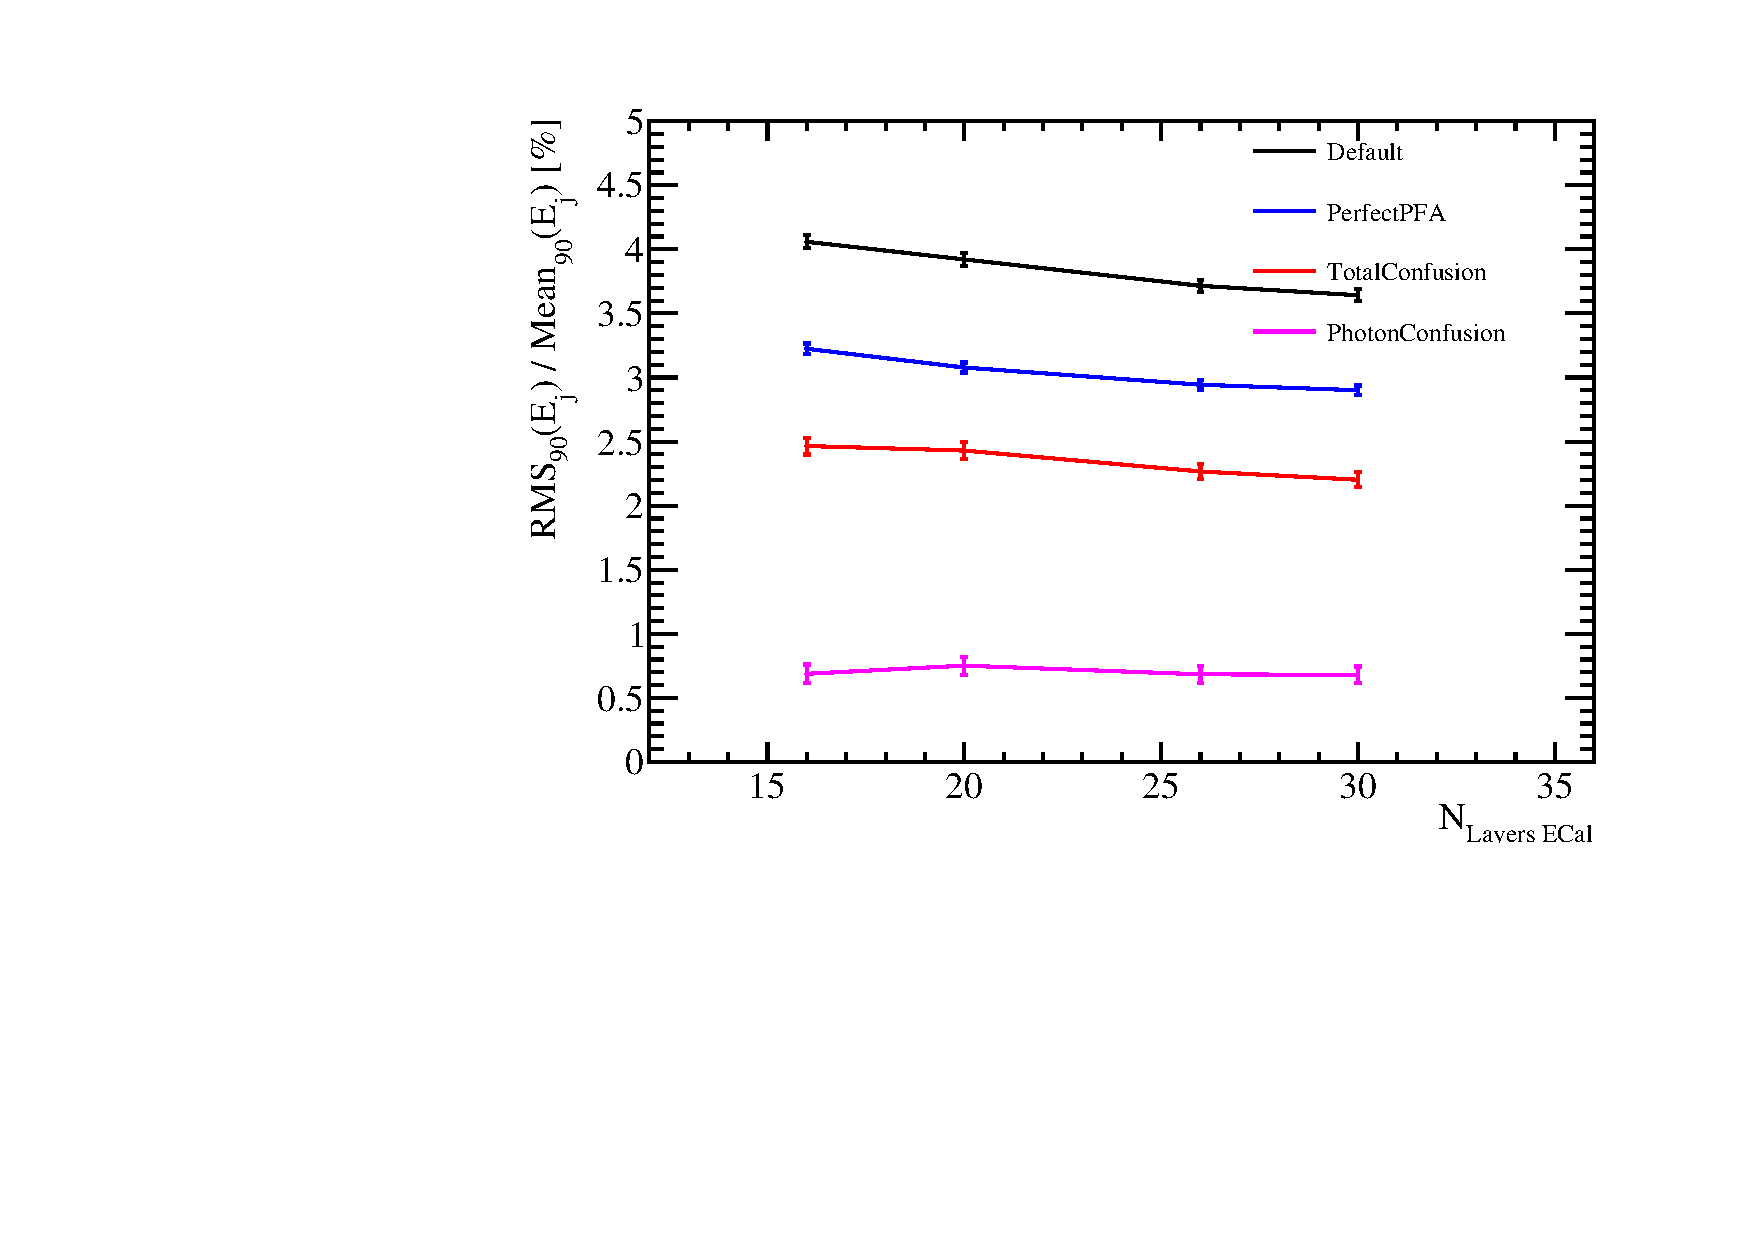
\includegraphics[width=0.5\textwidth]{OptimisationStudies/Plots/JetEnergyResolutions/JER_vs_ScintillatorECalNumberofLayers_91GeV_DiJet_Breakdown.pdf}} \hfill
\subfloat[]{\label{fig:ecalsinlayers250break}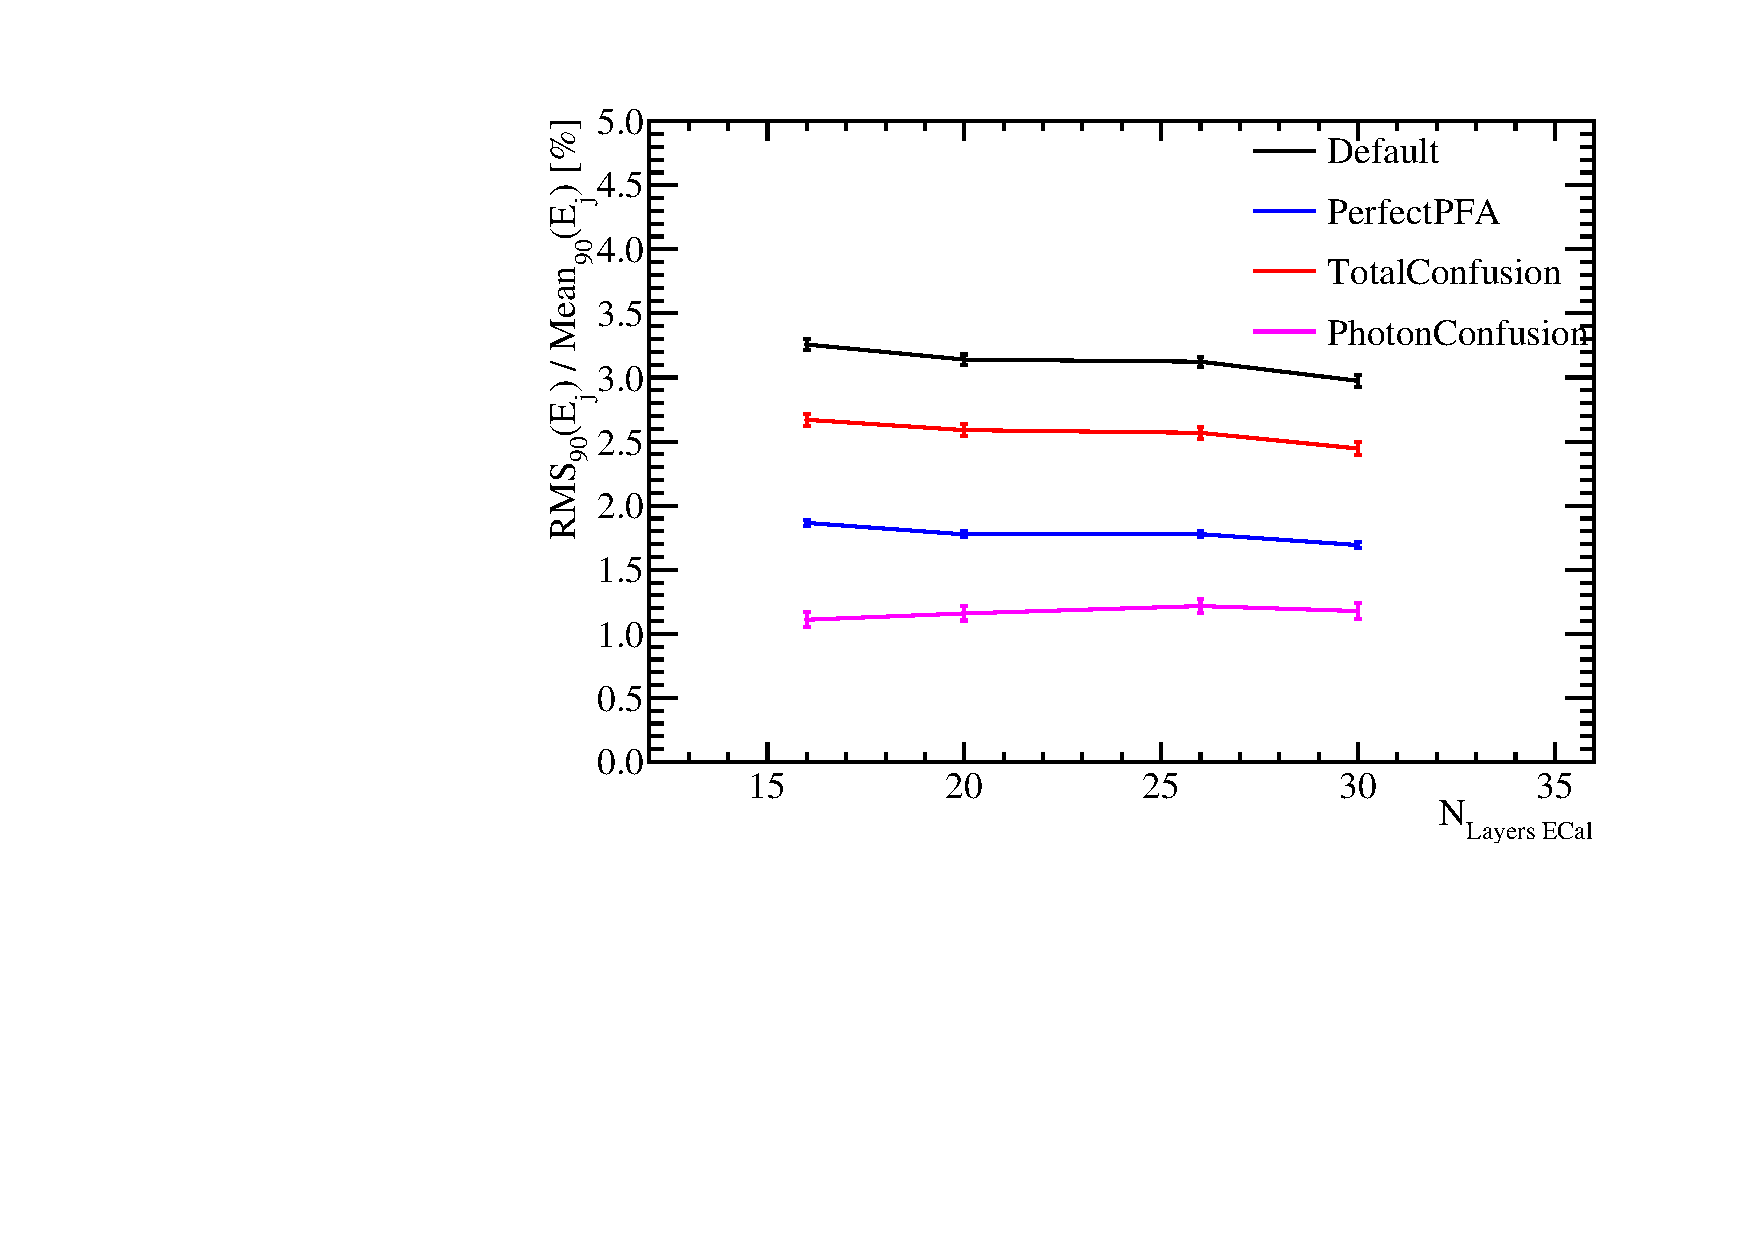
\includegraphics[width=0.5\textwidth]{OptimisationStudies/Plots/JetEnergyResolutions/JER_vs_SiliconECalNumberofLayers_500GeV_DiJet_Breakdown.pdf}}
\subfloat[]{\label{fig:ecalscnlayers250break}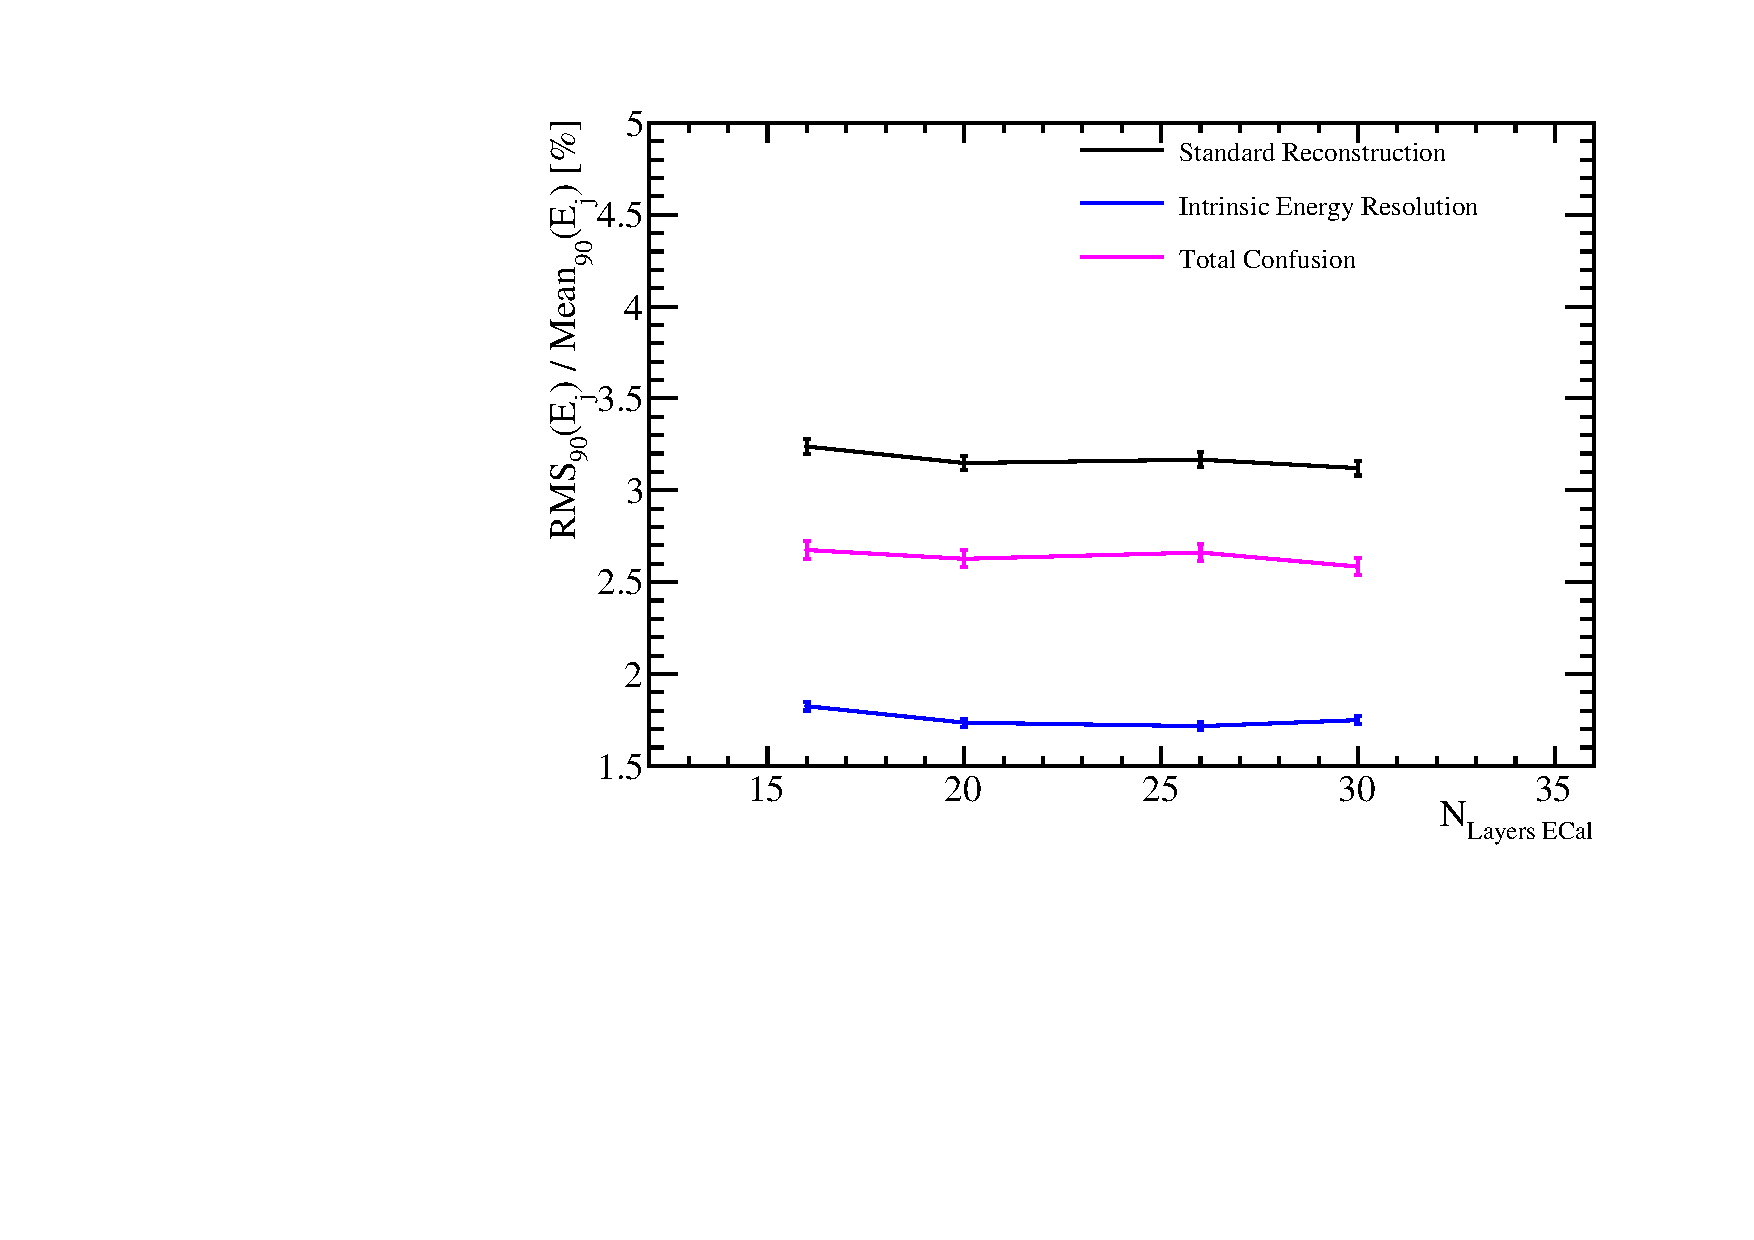
\includegraphics[width=0.5\textwidth]{OptimisationStudies/Plots/JetEnergyResolutions/JER_vs_ScintillatorECalNumberofLayers_500GeV_DiJet_Breakdown.pdf}}
\caption[The contributions to the jet energy resolution as a function of number of layers in the ECal using the nominal ILD detector model for \protect\subref{fig:ecalsinlayers45break} the silicon ECal option and 45~GeV jets, \protect\subref{fig:ecalscnlayers45break} the scintillator ECal option and 45~GeV jets, \protect\subref{fig:ecalsinlayers250break} the silicon ECal option and 250~GeV jets and \protect\subref{fig:ecalscnlayers250break} the scintillator ECal option and 250~GeV jets.  The black curves correspond to the standard reconstruction, the blue curves to the intrinsic energy resolution contribution to the jet energy resolution, the red curves to the confusion contribution to the jet energy resolution and the magenta curves to the confusion contribution to the jet energy resolution related solely to $\gamma$ reconstruction.]{The contributions to the jet energy resolution as a function of number of layers in the ECal using the nominal ILD detector model for \protect\subref{fig:ecalsinlayers45break} the silicon ECal option and 45~GeV jets, \protect\subref{fig:ecalscnlayers45break} the scintillator ECal option and 45~GeV jets, \protect\subref{fig:ecalsinlayers250break} the silicon ECal option and 250~GeV jets and \protect\subref{fig:ecalscnlayers250break} the scintillator ECal option and 250~GeV jets.  The black curves correspond to the standard reconstruction, the blue curves to the intrinsic energy resolution contribution to the jet energy resolution, the red curves to the confusion contribution to the jet energy resolution and the magenta curves to the confusion contribution to the jet energy resolution related solely to $\gamma$ reconstruction.}
\label{fig:ecalnlayersbreak}
\end{figure}

Increasing the number of layers in the ECal is beneficial to the intrinsic energy resolution and the jet energy resolution, particularly for low jet energies.  Separation of the W and Z hadronic decays should be possible for ILC like energies given there are at least 26 layers in the ECal, however, it is desirable to have as large a number of layers as possible to benefit single $\gamma$ energy resolution.  

%========================================================================================

\subsection{ECal Active Material}
In sections \ref{sec:ecalcells} and \ref{sec:ecalnlayers} the performance of the ECal was reported for both the silicon and scintillator options and to a large extent the performance of the two options was similar, but not identical:

\begin{itemize}
\item The intrinsic energy resolution of the silicon ECal option is better than that of a scintillator option for high energies, see figures \ref{fig:ecalsinominalres} and \ref{fig:ecalscnominalres}.  This is most likely due to the implementation of Birks' law \cite{BirksLaw} for scintillator active materials., which states:
\begin{equation}
\frac{d\mathcal{L}}{dx} \propto \times \frac{dE/dx}{1+k_{B}dE/dx}\text{ ,}
\end{equation}
where $\frac{d\mathcal{L}}{dx}$ is the light yield per unit path length, $dE/dx$ is the energy deposited per unit path length and $k_{B}$ is a material property constant.  For large energy deposits per unit length, such as those found in high energy $\gamma$ events, the light yield saturates causing a degradation in the energy resolution.  Based on a comparison with the silicon ECal option performance, this effect starts to degrade the energy resolution for the scintillator option around 50~GeV.  However, the degradation in energy resolution up to 100~GeV is relatively small.
\item The "dead" region due to the presence of the MPPC in the simulation of the scintillator ECal option degrades performance of the detector for small transverse granularities, see figure \ref{fig:ecalcellsizegamma}.
\end{itemize}

In summary, the performance of the two options, in terms of energy and jet energy resolution, are similar, meaning no clear option is preferred.  However, the silicon option is preferred when manufacture and implementation of the two models is compared.  While constructing silicon wafers to fit a $5 \times 5 \text{mm}^{2}$ square cell size is achievable, this would be extremely challenging for scintillator tiles.  To resolve this in actuality, the scintillator ECal option would have to use $5 \times 45 \text{mm}^{2}$ scintillator strips that are arranged in alternating directions in each ECal layer.  By combining information from neighbouring layers it becomes possible to effectively achieve a $5 \times 5 \text{mm}^{2}$ square cell size.  

%========================================================================================
%========================================================================================

\section{Hadronic Calorimeter Optimisation}
\label{sec:hcal}
The purpose of an hadroinc calorimeter (HCal) is to measures the energy deposits from hadronic showers.  The HCal in the default ILD detector model, summarised in table \ref{table:defaultildhcal}, is approximately 6 nuclear interaction lengths ($\lambda_{I}$) deep.  The ECal contributes approximately one $\lambda_{I}$ giving a total of $\approx 7 \lambda_{I}$, which is sufficient to contain jets at ILC like energies.  The longitudinal structure of this model consists of 48 readout layers each containing a 3 mm active layer of scintillator and a 20 mm absorber layer of iron.  

\begin{table}[h!]
\centering
\begin{tabular}{ l l}
\hline
Parameter & Default Value \\
\hline
Cell Size & $30 \times 30 \text{mm}^{2}$ square cells \\
Number of Layers & 48 readout layers \\
Active Material Choice & Scintillator \\
Active Material Thickness & 3 mm  \\
Absorber Material Choice & Steel \\
Absorber Material Thickness & 20 mm \\
\hline
\end{tabular}
\caption[The configuration of the HCal in the nominal ILD detector model.]{The configuration of the HCal in the nominal ILD detector model.}
\label{table:defaultildhcal}
\end{table}
% Nuclear interaction length iron 167.7mm
% Nuclear interaction length tungsten 99.46mm 
% Nuclear interaction length silicon 465.2mm 
% Nuclear interaction length polystyrene 770.7mm

There are several readout approaches under consideration for the HCal including fully analogue, fully digital and semi-digital.  The analogue readout measures the energy within each HCal cell using a continuous spectrum of measurements, while the digital readout only produces a response if the energy deposited within a calorimeter cell is above a given threshold.  The semi-digital approach mirrors that of the digital approach, but has three responses each with a different energy threshold.  While the energy resolution for digital calorimeters is not as good as that of analogue calorimeters, it is possible to construct smaller cell sizes using a digital readout.  In traditional calorimetry, a digital calorimeter would give a worse jet energy resolution than the analogue equivalent, however, that is not necessarily the case in particle flow calorimetry.  If a digital calorimeter could be realised with a much small cell size than the analogue equivalent, then the affect of confusion in the digital calorimeter may be reduced so much that it compensates for any loss to intrinsic energy resolution.  In the following studies optimisation of the analogue HCal is presented as this is the readout approach used in the nominal ILD detector model.  

A number of options were simulated where the following parameters in the HCal were varied:
\begin{itemize}
\item Cell size:  This is crucial for successful application particle flow calorimetry for making associations between clusters of calorimeter hits and charged particle tracks.  It is expected that the intrinsic energy resolution be invariant to changes in the HCal cell size.  
\item Number of readout layers i.e. varying total depth of HCal:  The number of layers in the HCal are varied, however, the thickness of those layers match those of the nominal ILD HCal design.  This means the total depth of the HCal in $\lambda_{I}$ is changing.  It is expected that this study will determine the effect of leakage of energy out of the back of the HCal.
\item Sampling frequency:   This involves changing the of readout layers in the HCal while simultaneously changing the thicknesses of the active and absorber layers to keep the total number of $\lambda_{I}$ in the HCal constant.  As this modifies the sampling of particle showers in the HCal, this will affect the intrinsic energy resolution of the HCal.
\item Sampling fraction:  This is the ratio of the active medium thickness to the absorber medium thickness.  This controls how particle showers within the calorimeter are sampled.  In this study the total depth of the HCal in $\lambda_{I}$ is held constant between detector models.  
\item Absorber material choice:  Two options have been considered: steel and tungsten.  This choice dictates the growth and propagation of hadronic showers and so plays a crucial role in calorimetry.  
\end{itemize}

%========================================================================================

\subsection{HCal Cell Size}
\label{sec:hcalcells}
The HCal cell size is an important detector parameter in the application of particle flow calorimetry.  Smaller HCal cell sizes will lead to a finer spatial resolution that can be used to better separate charged and neutral particle calorimetric energy deposits.  On the other hand, this will also lead to an increase in the number of readout channels that will raise the cost of the calorimeter.  Therefore, it is highly desirable to achieve the optimal physics performance using the largest cell size possible.  The nominal ILD HCal has a 30 mm square cell size and in this study the following square cell sizes were considered; 10 mm, 20 mm, 30 mm, 40 mm, 50 mm and 100 mm.  

The energy resolution for 50~GeV $\text{K}^{0}_{L}$ events as a function of cell size in the HCal is shown in figure \ref{fig:hcalcellser}.  These $\text{K}^{0}_{L}$ samples will deposit energy primarily within the HCal, making them appropriate events to consider when determining the performance of the HCal.  However, a non-neglibile amount of energy will also be deposited within the ECal.  Therefore, these energy resolutions represent the intrinsic energy resolution of the ILD detector as a whole and not purely that of the HCal.  It is clear that there is no strong dependency on the energy resolution of the $\text{K}^{0}_{L}$ as a function of the HCal cell size.  There are small fluctuations in the energy resolution that are most likely due to variations in applying the calibration procedure and the tuning of the optimal HCal cell truncation, described in section \ref{sec:hcalcelltruncation}.  The precision on the optimal cell truncation is worse for large HCal cell sizes as the truncations considered in the optimisation are focused around the optimal truncation for the nominal ILD HCal.  

\begin{figure}[h!]
\centering
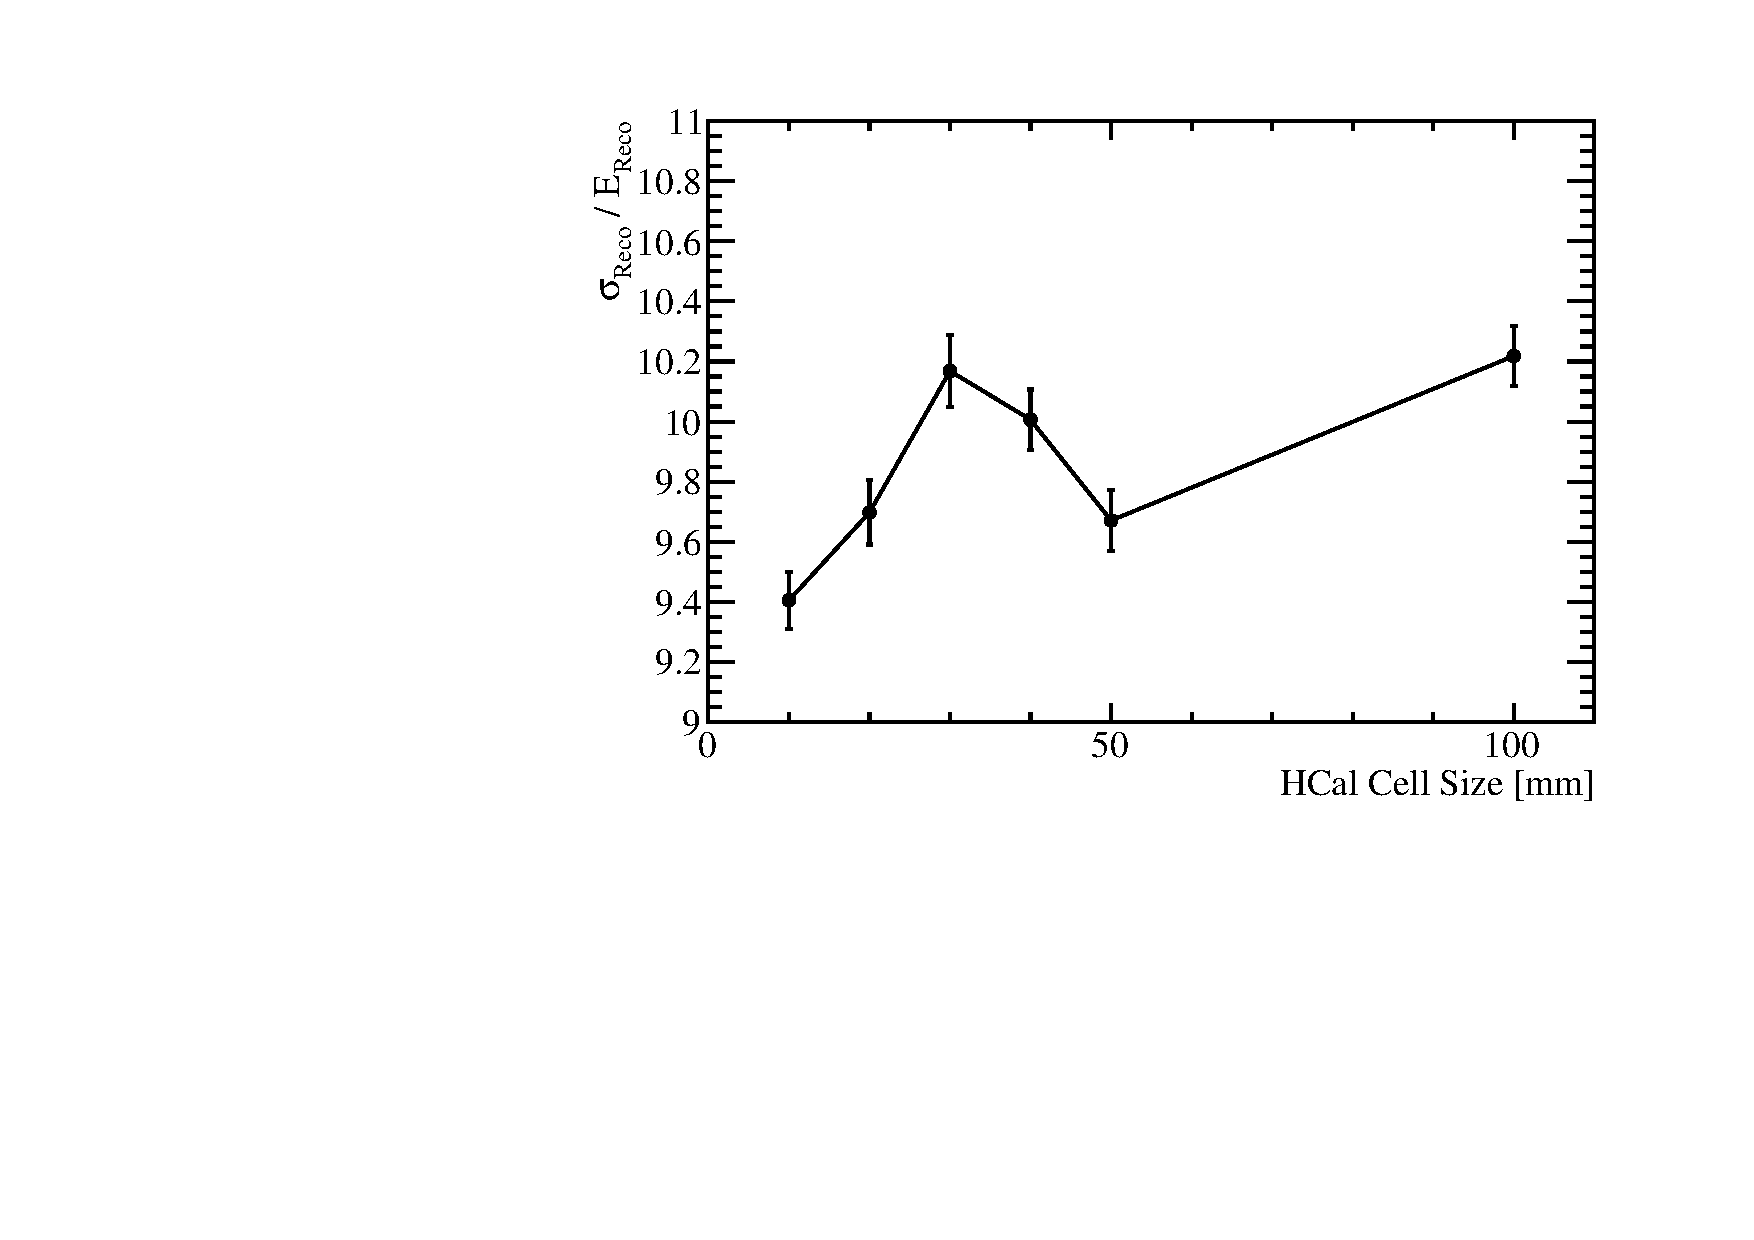
\includegraphics[width=0.5\textwidth]{OptimisationStudies/Plots/EnergyResolution/ER_vs_HCalCellSize_50GeVKaon0L.pdf}
\caption[The energy resolution as a function of HCal cell size for 50~GeV $\text{K}^{0}_{L}$ events using the nominal ILD detector model.]{The energy resolution as a function of HCal cell size for 50~GeV $\text{K}^{0}_{L}$ events using the nominal ILD detector model.}
\label{fig:hcalcellser}
\end{figure}

As a smaller HCal cell size will lead to better separation of charged and neutral hadron calorimetric energy deposits, it is expected that the confusion contribution to the jet energy resolution will be reduced by using smaller HCal cell sizes.  The jet energy resolution as a function of cell size in the HCal shown in figure \ref{fig:hcalcellsize}.  At low jet energies there is no strong dependency of the jet energy resolution on the HCal cell size, which is as expected from the $\text{K}^{0}_{L}$ energy resolution study.  For high energy jets there is a clear dependence, with lower HCal cell sizes leading to better jet energy resolutions.  Examining the different contributions to the jet energy resolution, shown in figure \ref{fig:hcalcellsizebreak} it can be seen that the intrinsic energy resolution contribution is largely invariant to changes in the HCal cell size.  Instead it is the confusion contribution that drives the overall trend in the jet energy resolution.  This is particularly clear at high jet energies where the confusion contribution to the jet energy resolution dominates that of the intrinsic energy resolution contribution.  At high jet energies smaller HCal cell sizes clearly lead to a reduction in the effect of confusion.  At low jet energies the trend in confusion is less clear, as the confusion contribution is less dominant, but a reduction in the effect of confusion with decreasing cell size is still visible for all but the smallest HCal cell size.  The most likely cause of the increase in confusion for the smallest HCal cell size at low energies is tuning of the PandoraPFA algorithms to the nominal ILD HCal cell size.  Furthermore, for both energies the photon confusion is largely invariant to changes in the HCal cell size.  This indicates that the changes in confusion when varying the HCal cell size are due to pattern recognition improvements related to hadrons.

\begin{figure}[h!]
\centering
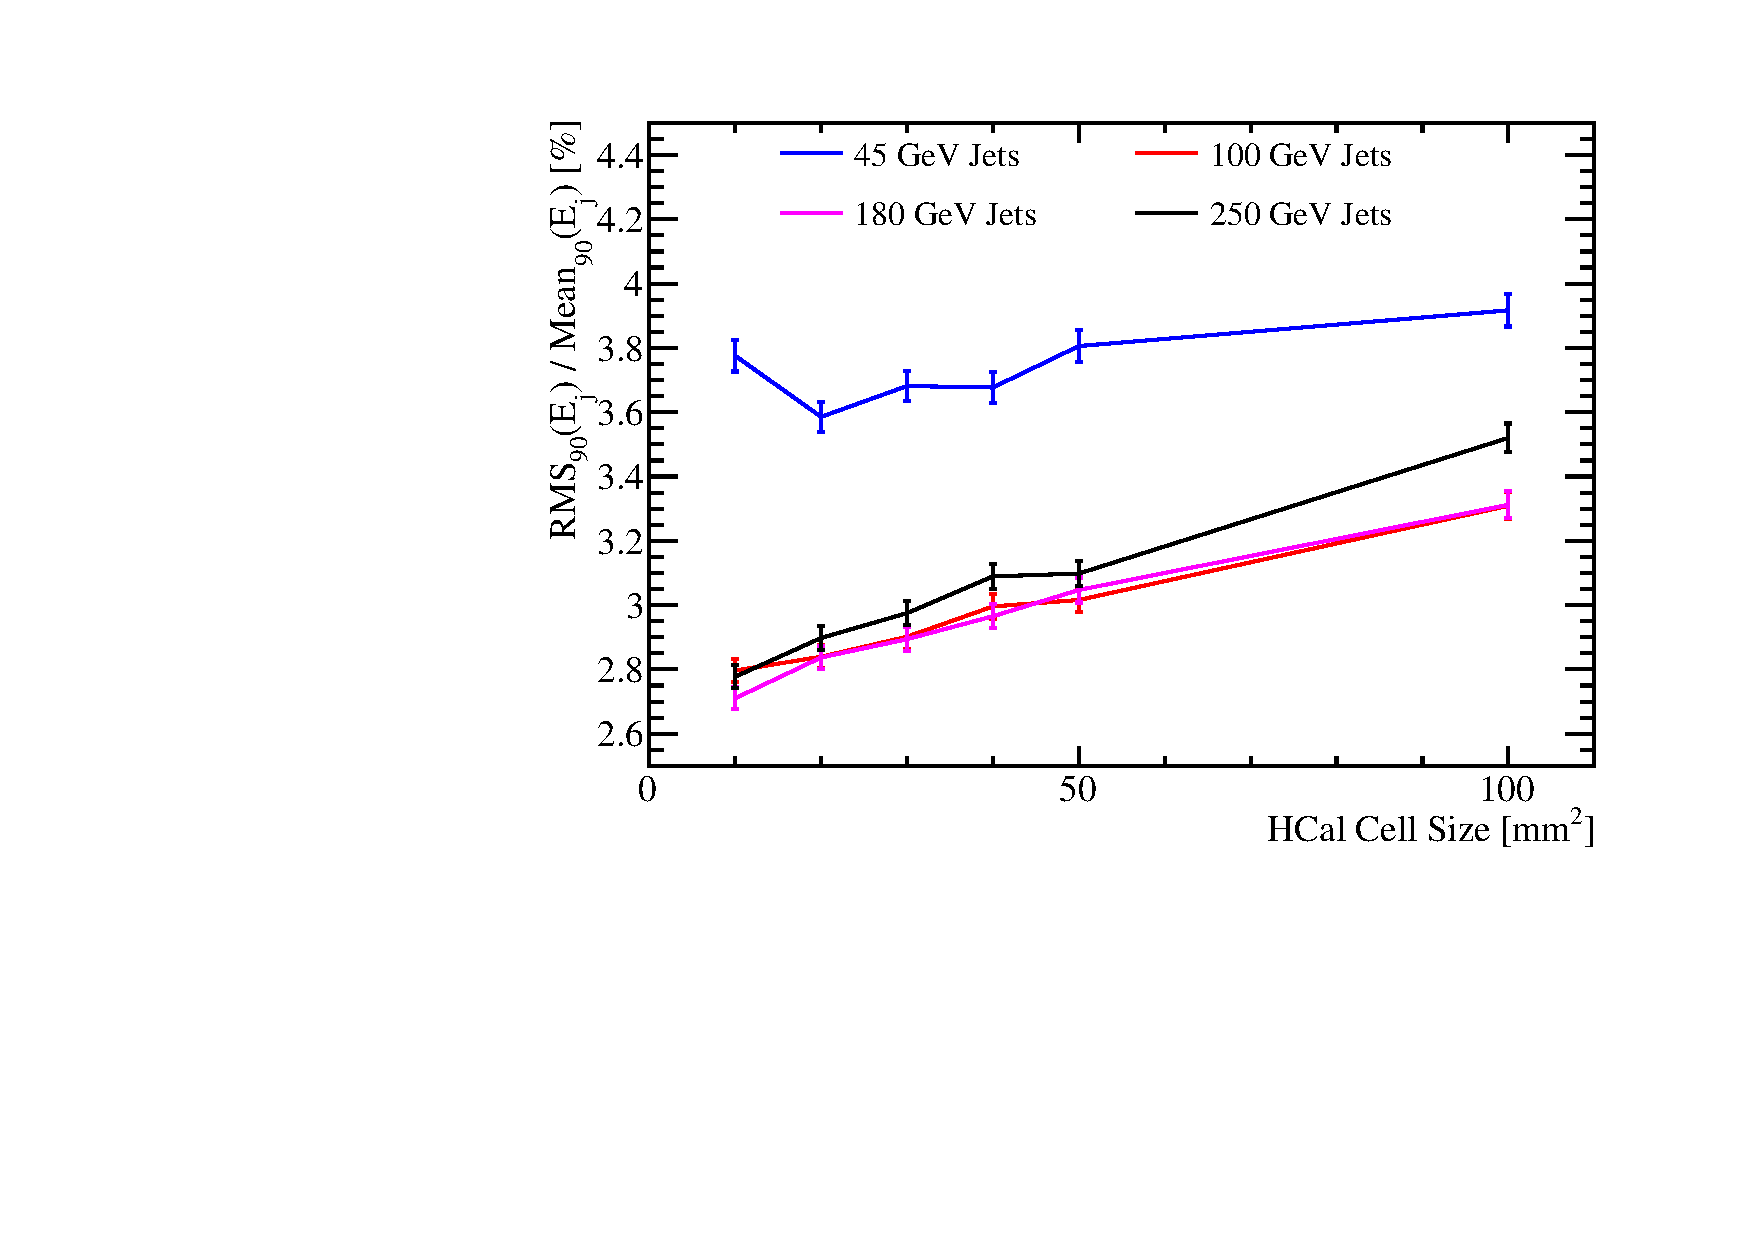
\includegraphics[width=0.5\textwidth]{OptimisationStudies/Plots/JetEnergyResolutions/JER_vs_HCalCellSize.pdf}
\caption[The jet energy resolution as a function of HCal cell size for various jet energies using the nominal ILD detector model.]{The jet energy resolution as a function of HCal cell size for various jet energies using the nominal ILD detector model.}
\label{fig:hcalcellsize}
\end{figure}

\begin{figure}[h!]
\centering
\subfloat[]{\label{fig:hcalcellsize45break}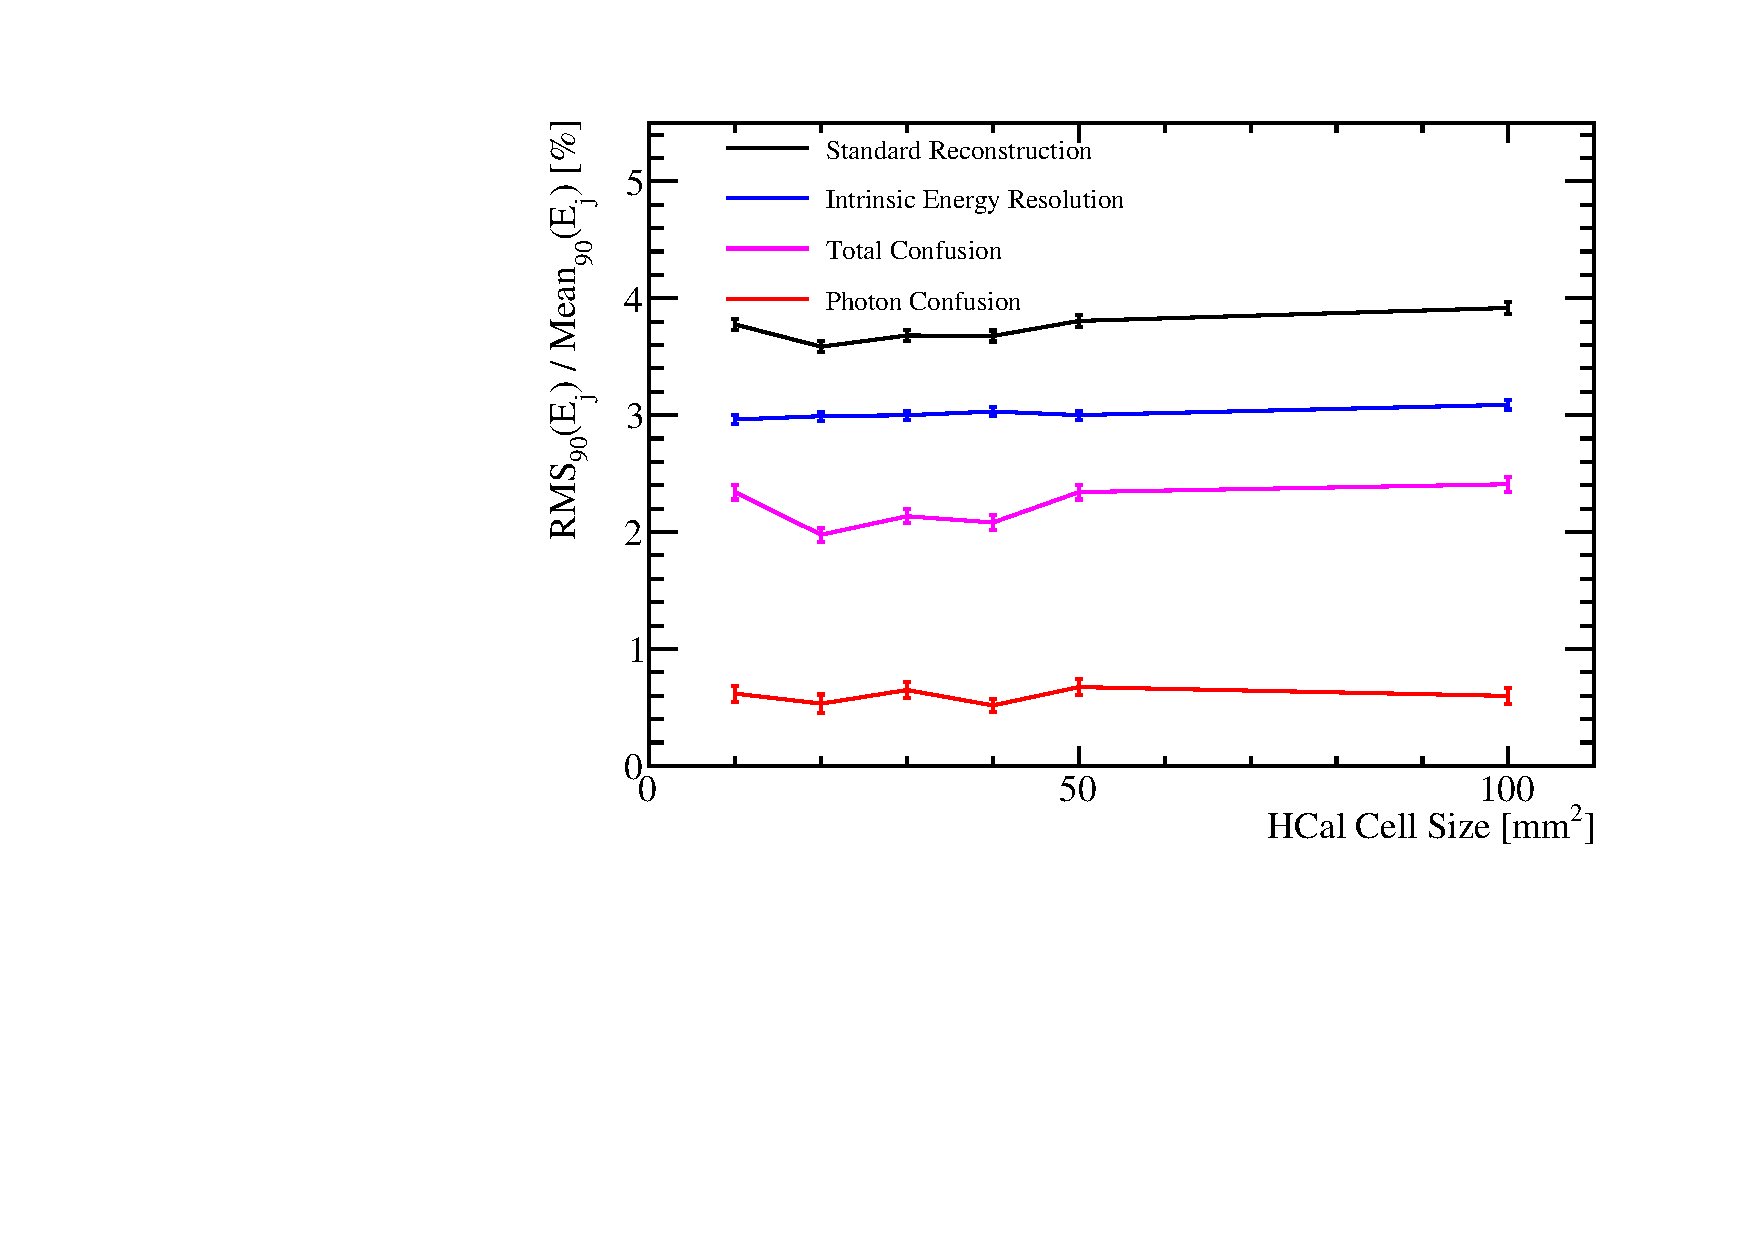
\includegraphics[width=0.5\textwidth]{OptimisationStudies/Plots/JetEnergyResolutions/JER_vs_HCalCellSize_91GeV_DiJet_Breakdown.pdf}}
\subfloat[]{\label{fig:hcalcellsize250break}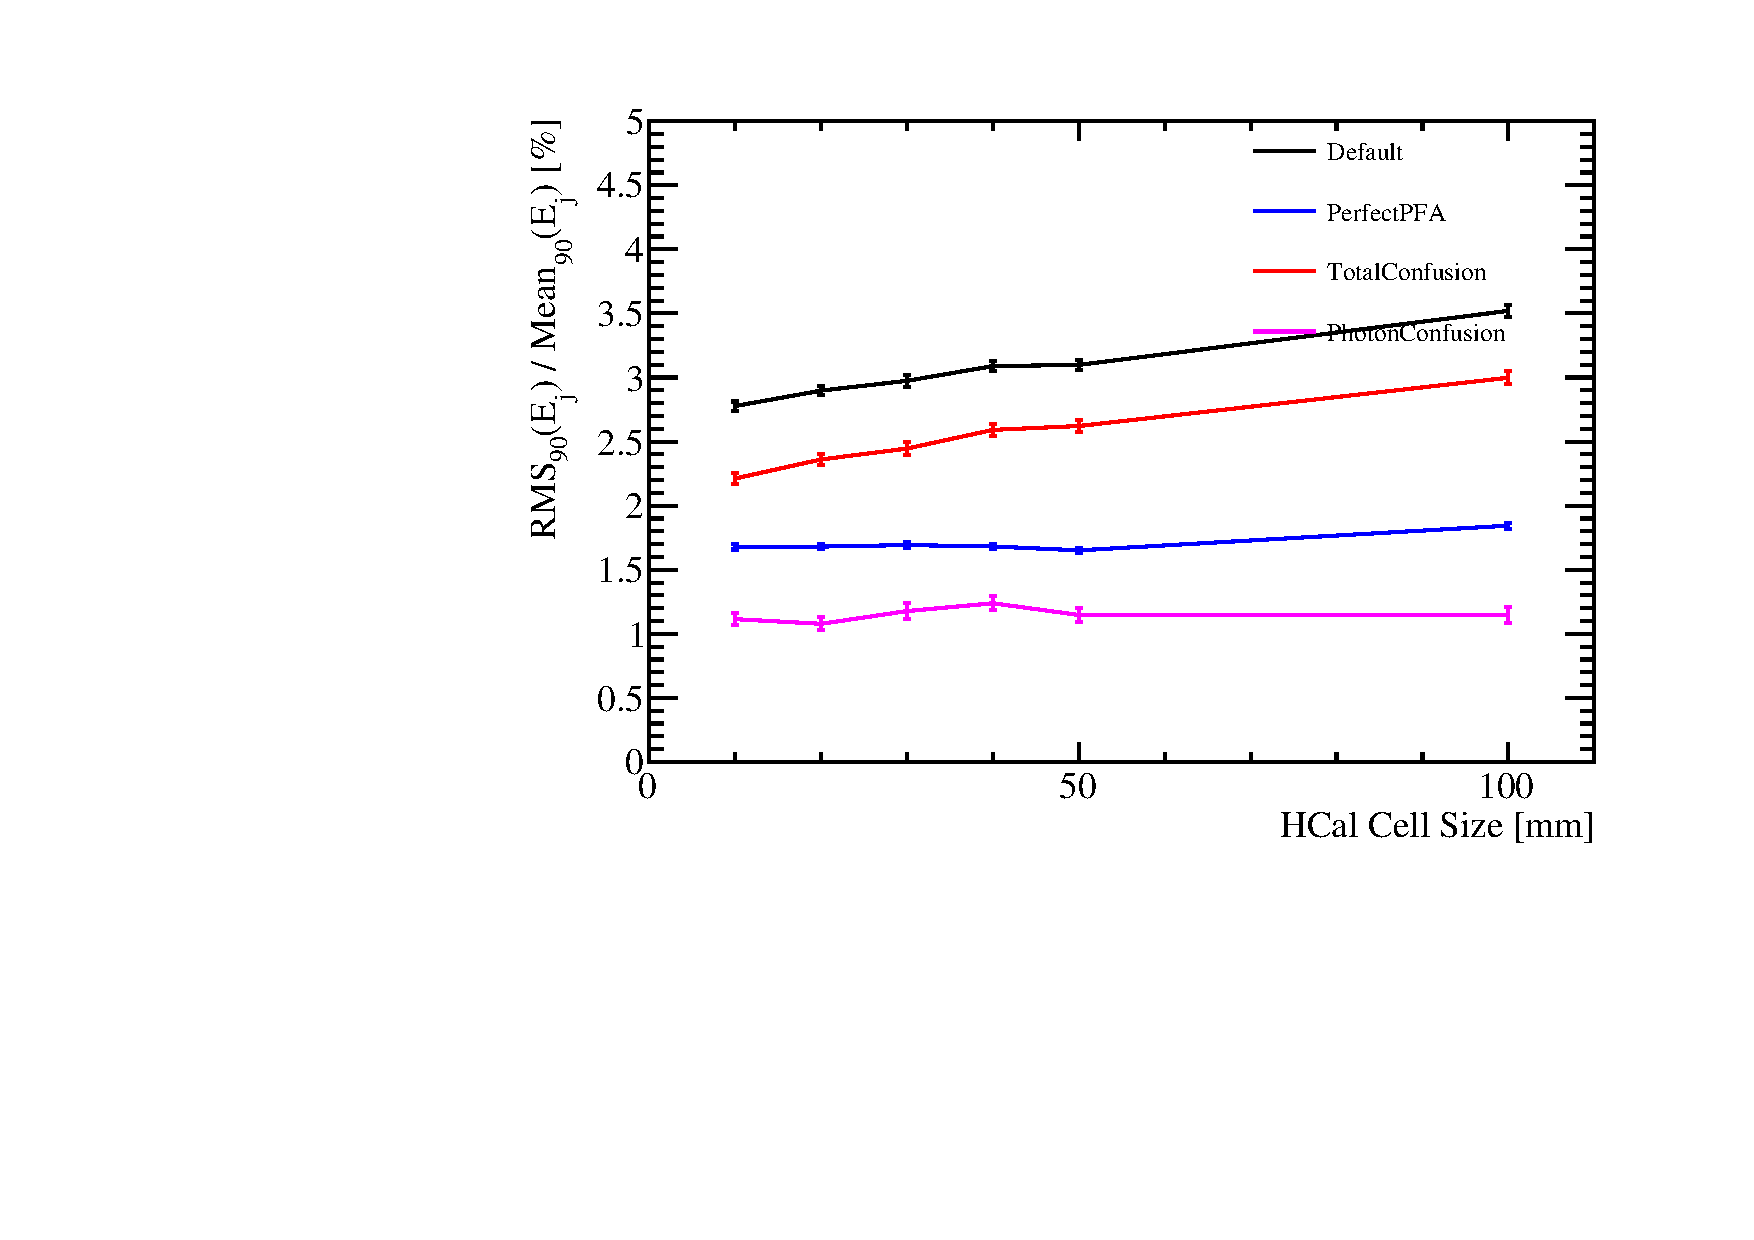
\includegraphics[width=0.5\textwidth]{OptimisationStudies/Plots/JetEnergyResolutions/JER_vs_HCalCellSize_500GeV_DiJet_Breakdown.pdf}}
\caption[The contributions to the jet energy resolution as a function of HCal cell size using the nominal ILD detector model for \protect\subref{fig:hcalcellsize45break} 45~GeV jets and \protect\subref{fig:hcalcellsize250break} 250~GeV jets.  The black curves correspond to the standard reconstruction, the blue curves to the intrinsic energy resolution contribution to the jet energy resolution, the red curves to the confusion contribution to the jet energy resolution and the magenta curves to the confusion contribution to the jet energy resolution related solely to $\gamma$ reconstruction.]{The contributions to the jet energy resolution as a function of HCal cell size using the nominal ILD detector model for \protect\subref{fig:hcalcellsize45break} 45~GeV jets and \protect\subref{fig:hcalcellsize250break} 250~GeV jets.  The black curves correspond to the standard reconstruction, the blue curves to the intrinsic energy resolution contribution to the jet energy resolution, the red curves to the confusion contribution to the jet energy resolution and the magenta curves to the confusion contribution to the jet energy resolution related solely to $\gamma$ reconstruction.}
\label{fig:hcalcellsizebreak}
\end{figure}

A comparison of the results from the ECal and HCal cell size optimisation studies shows that the jet energy resolution has a much stronger dependency on the ECal cell size that the HCal cell size.  This is to be expected as in the particle flow paradigm $\approx 30\%$ of jet energy is recorded in the ECal, while only $\approx 10\%$ is recorded in the HCal meaning the potential effect of double counting and omitting energy deposits, i.e. confusion, is greater in the ECal than the HCal.  Therefore, minimising confusion in the ECal should be more crucial for the overall jet energy resolution, which is what is observed.  Furthermore, as PandoraPFA groups calorimeter hits together using a cone clustering approach, identifying the start of a particle shower is key for determining how calorimeters hits are grouped together deeper into the calorimeters.  In effect, this means the grouping of calorimeter hits in the HCal heavily relies upon information gathered in the ECal.  Therefore, if the ECal performance is sufficiently good, even with corse HCal cell sizes excellent performance can be achieved.  

In summary, the confusion contribution to the jet energy resolution falls as the HCal cell size is reduced, while the intrinsic energy resolution of the detector is largely invariant to changes in the HCal cell size.  As this dependancy is relatively weak, even the use of 100 mm square HCal cell sizes would be enough to allow for separation of the hadronic decays of W and Z bosons at ILC like energies.  However, as jet energy resolution does improve with decreasing cell sizes it is desirable to have as small a HCal cell size as possible.

%========================================================================================

\subsection{HCal Number of Layers}
\label{sec:hcalnlayers}
A number of detector models were simulated where the total number of layers in the HCal was varied.  In contrast to the sampling frequency study, the thickness of the HCal layers were not modified.  Changing the number of layers in this way leads to a change in the total thickness of the calorimeter.  It is expected that this study will determine what effects, if any, leakage of energy out of the back of the calorimeter will have on detector performance.  The cost of the HCal is proportional to the number of readout channels, which is proportional to the number of layers used in the HCal.  Therefore, minimising the number of layers, while retaining excellent physics performance is vital.  For this study detector models were simulated with a HCal containing 36, 42, 48 (nominal), 54 and 60 layers. 

It is expected that the energy resolution of the detector will improve when the number of layers in the HCal is increased as fewer events should suffer from the effects of leakage.  Any improvements seen by increasing the number of layers in the HCal is expected only up to a point, as beyond this point the majority of hadronic showers will be fully contained making additional HCal layers redundant.  The energy resolution as a function of number of layers in the HCal for 50~GeV $\text{K}^{0}_{L}$ is shown in figure \ref{fig:hcalnfixedlayerser}.  The energy resolution becomes worse as the number of layers in the HCal is reduced below 48 layers, while above this point additional layers do not change the energy resolution.  This indicates that the majority of hadronic showers at this energy are fully contained by a 48 layer HCal.  However, as reducing the number of HCal layers to 36 only causes a small degradation in the neutral hadron energy resolution, it is feasible for the ILD to consider using a thinner HCal design.  

\begin{figure}[h!]
\centering
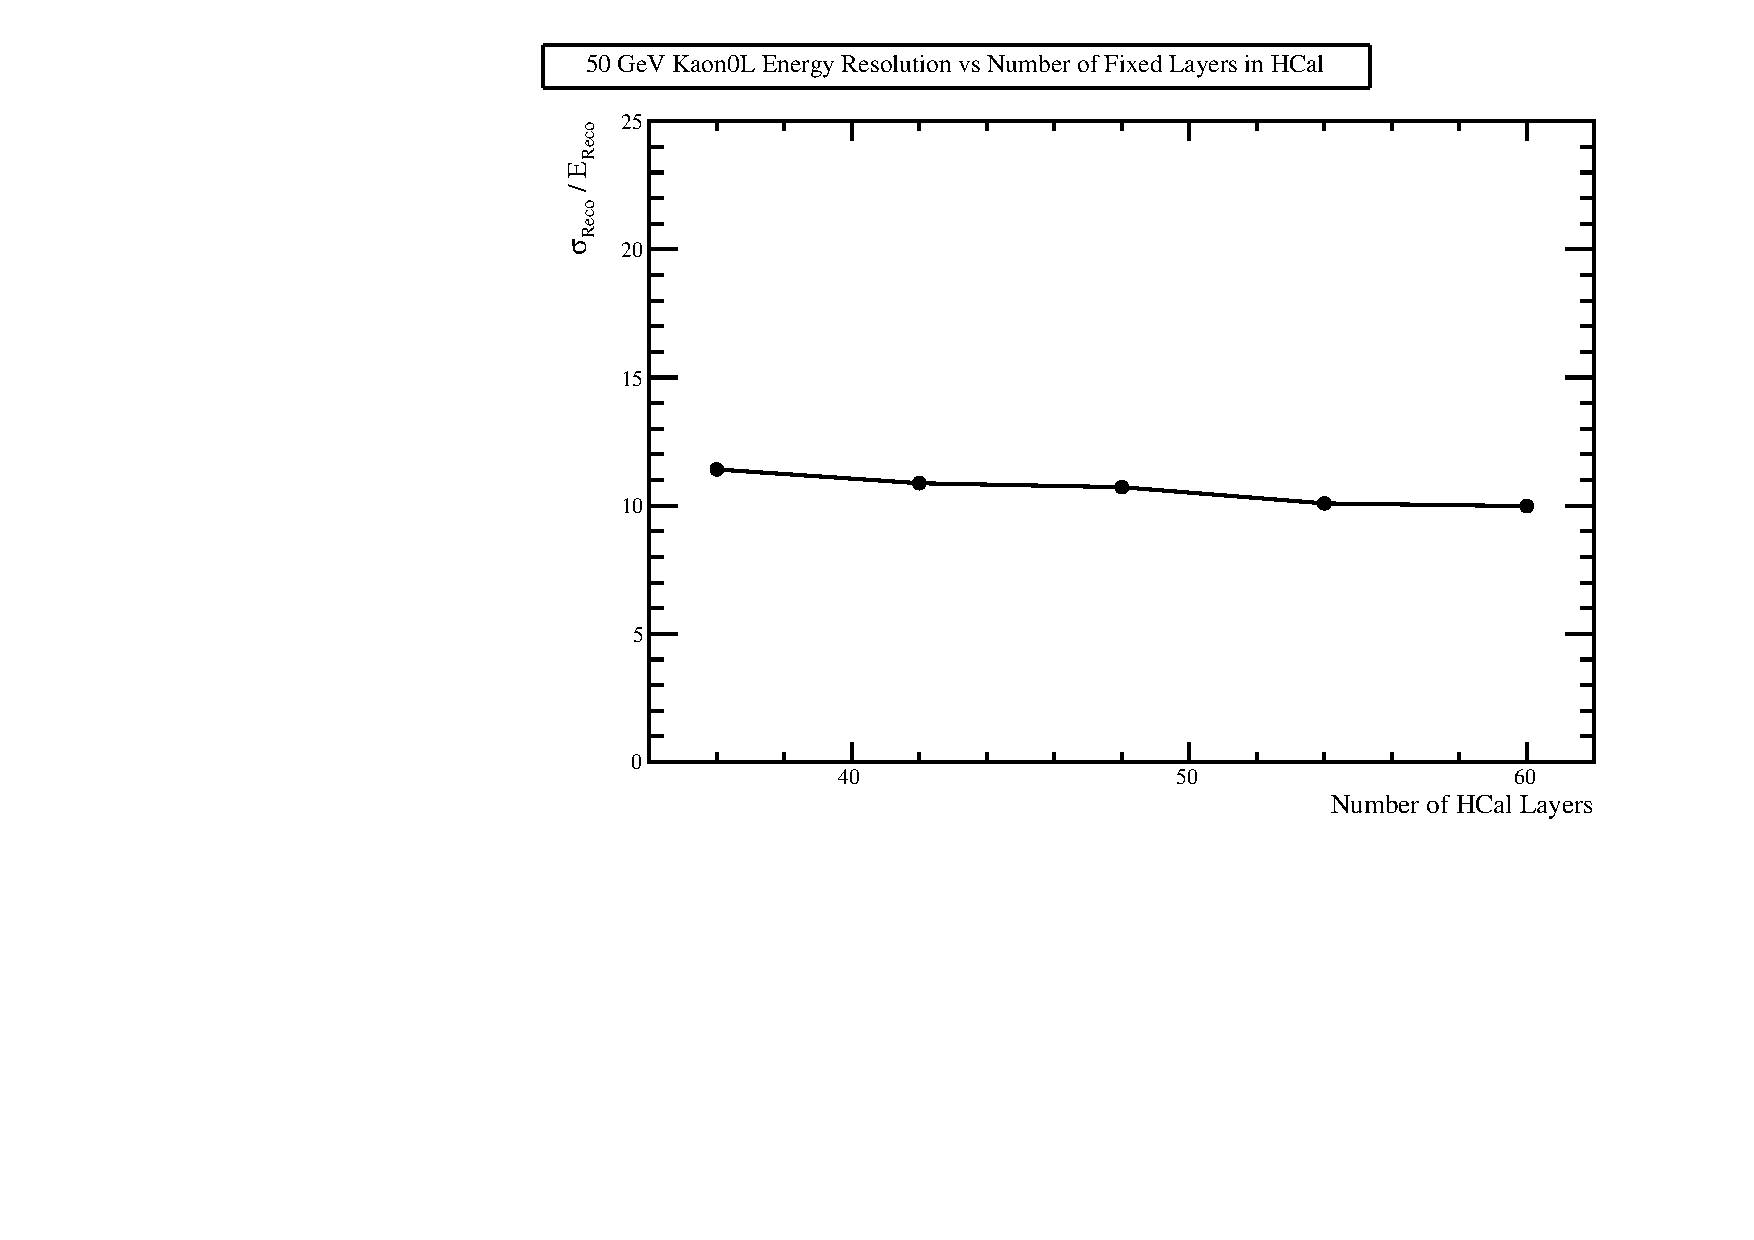
\includegraphics[width=0.5\textwidth]{OptimisationStudies/Plots/EnergyResolution/ER_vs_HCalNFixedLayers_50GeVKaon0L.pdf}
\caption[The energy resolution as a function of number of layers in the HCal for 50~GeV $\text{K}^{0}_{L}$ events using the nominal ILD detector model.]{The energy resolution as a function of number of layers in the HCal for 50~GeV $\text{K}^{0}_{L}$ events using the nominal ILD detector model.}
\label{fig:hcalnfixedlayerser}
\end{figure}

The trend in the 50~GeV $\text{K}^{0}_{L}$ energy resolution observed when varying the number of layers in the HCal is unlikely to be seen in the jet energy resolution as the trend weak and only a small fraction of jet energy is measured within the HCal.  However, the confusion contribution to the jet energy resolution is expected to change as errors will be introduced, in the association of charged particle tracks to clusters of calorimeters hits, if part of the cluster energy has leaked from the back of the calorimeter.  For example, if a particle shower from a charged particle suffers heavily from leakage there will be a large disparity between the track momentum and the energy it deposits within the calorimeter.  In that case, PandoraPFA will be overly aggressive in associating other calorimeter energy deposits to this track to account for the energy that has leaked out of the calorimeter, which will increase the confusion.  The jet energy resolution as a function of the number of layers in the HCal is shown in figure \ref{fig:hcalnfixedlayers}.  As expected for low energy jets, where intrinsic energy resolution dominates, the jet energy resolution is invariant to the number of layers, while for high jet energies, where confusion dominates, a larger number of layers benefits the jet energy resolution.  When examining the different contributions to the jet energy resolution, shown in figure \ref{fig:hcalnfixedlayersbreak}, it becomes clear that the confusion contribution that drives the observed trends.  The intrinsic energy resolution is largely invariant to changes to the number of HCal layers as only a small fraction of jet energy is recorded in the HCal.  Furthermore, the photon confusion is invariant to changes in the number of HCal layers, indicating that the change in the confusion contribution are originating from pattern recognition involving hadrons.

\begin{figure}[h!]
\centering
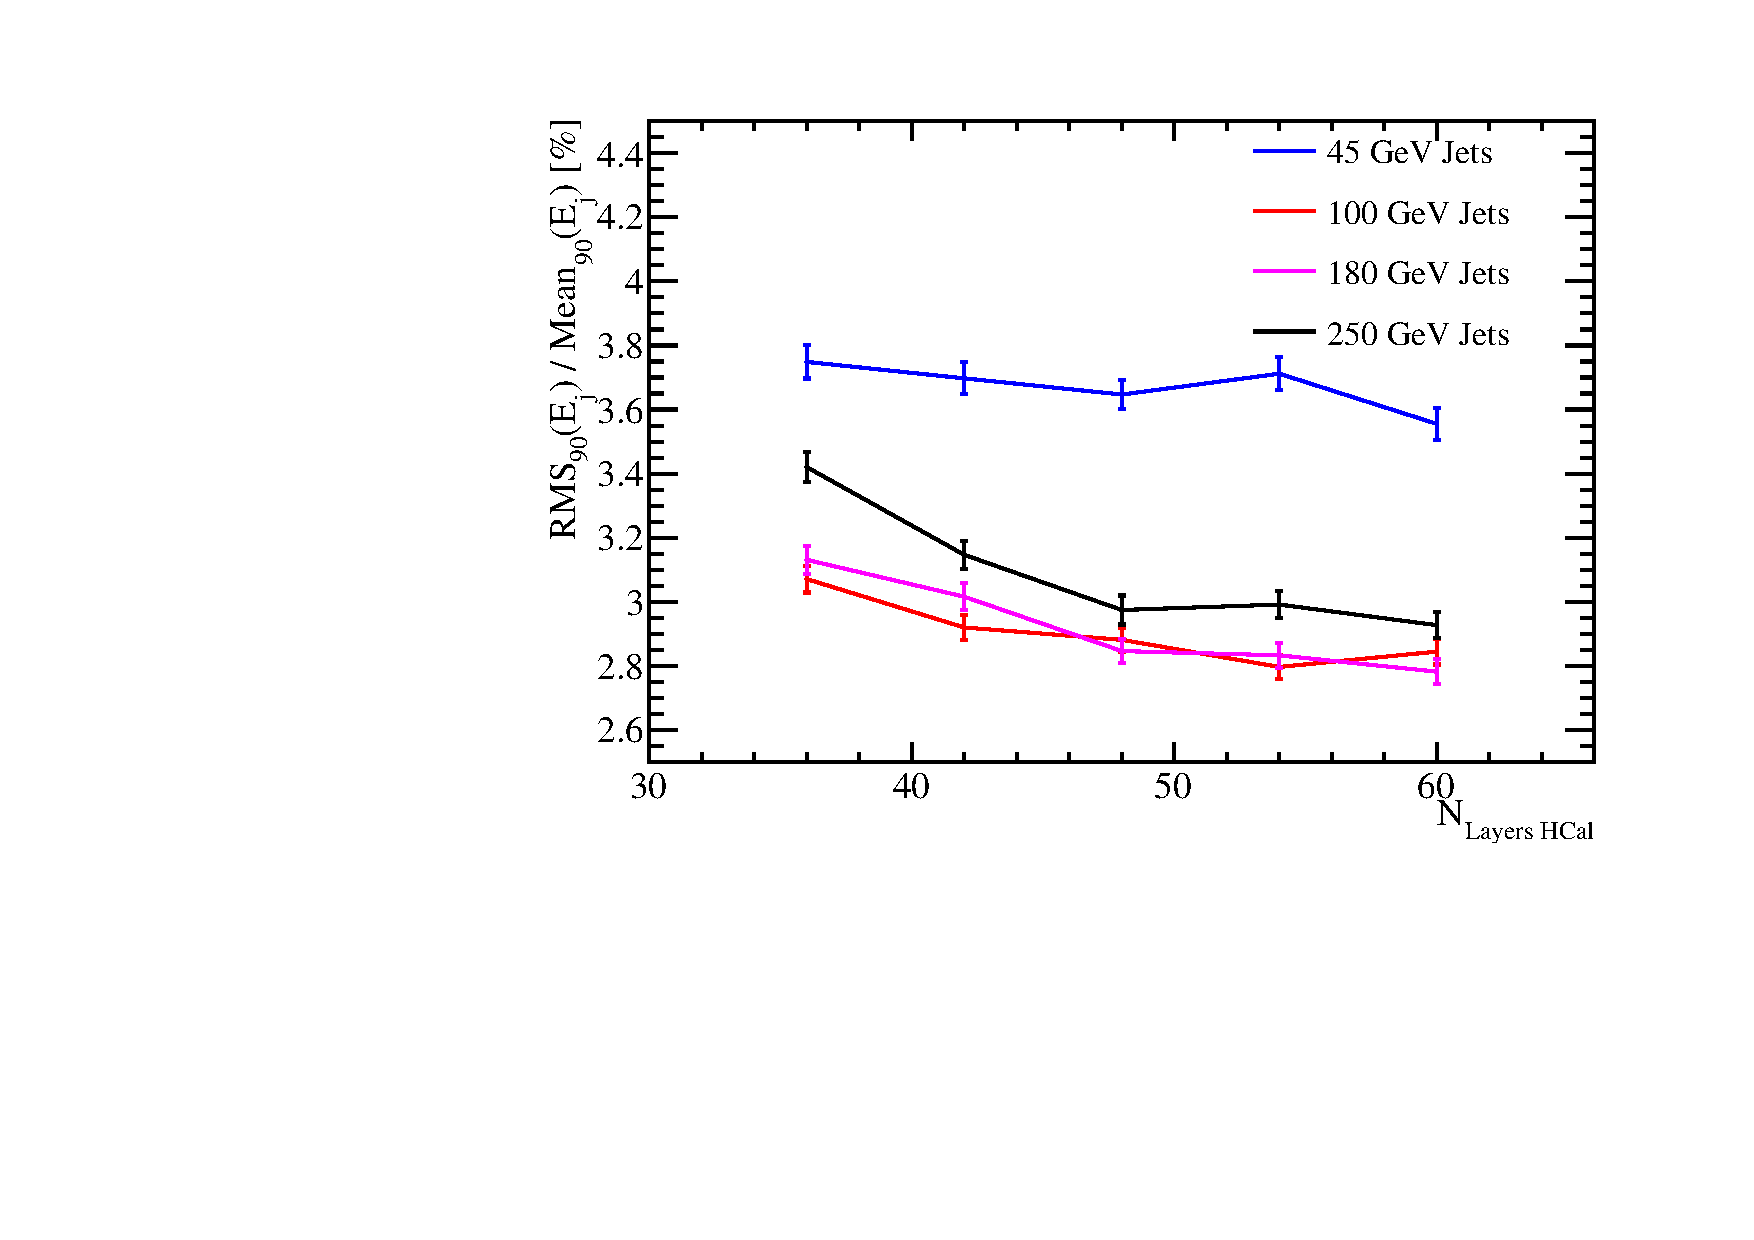
\includegraphics[width=0.5\textwidth]{OptimisationStudies/Plots/JetEnergyResolutions/JER_vs_NumberOfHCalLayersOfFixedDepth.pdf}
\caption[The jet energy resolution as a function of number of layers in the HCal for various jet energies using the nominal ILD detector model.]{The jet energy resolution as a function of number of layers in the HCal for various jet energies using the nominal ILD detector model.}
\label{fig:hcalnfixedlayers}
\end{figure}

\begin{figure}[h!]
\centering
\subfloat[]{\label{fig:hcalnfixedlayers45break}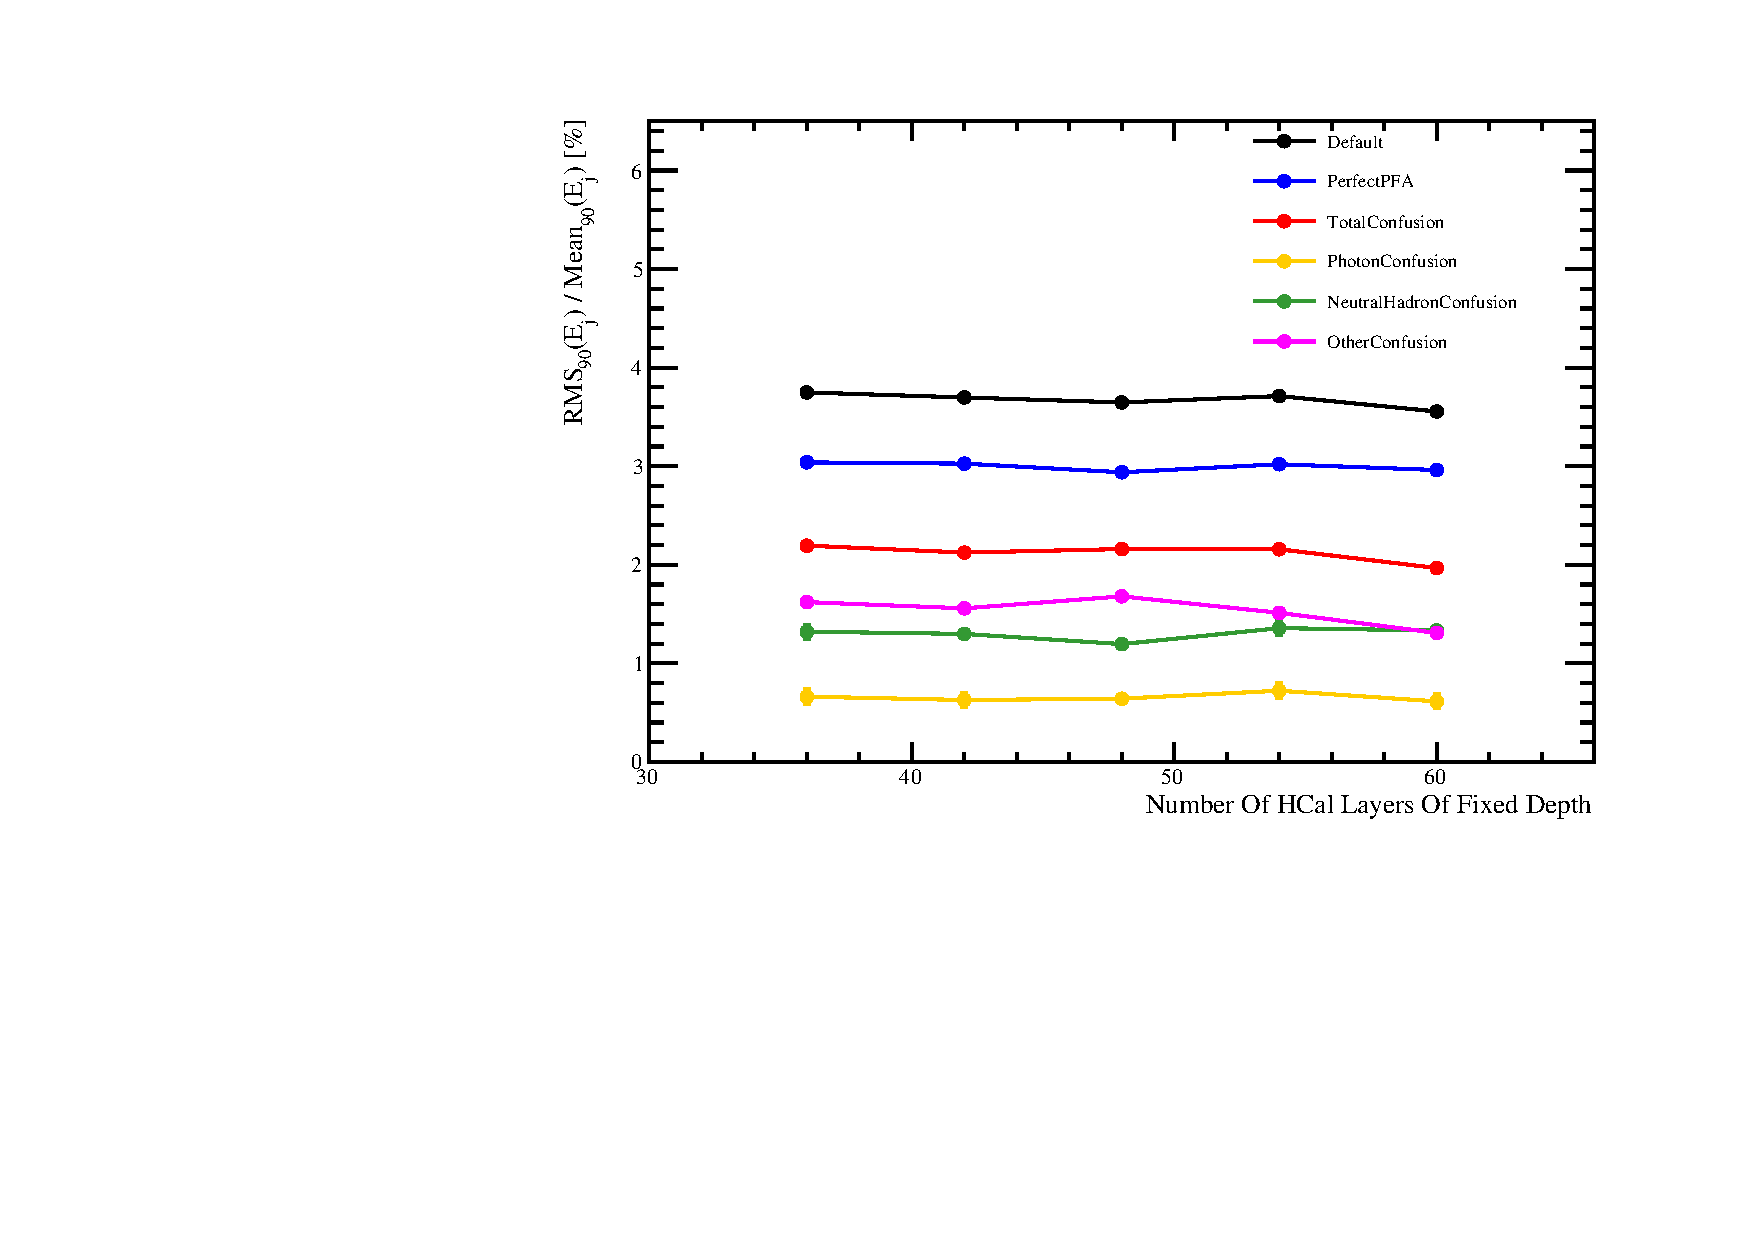
\includegraphics[width=0.5\textwidth]{OptimisationStudies/Plots/JetEnergyResolutions/JER_vs_NumberOfHCalLayersOfFixedDepth_91GeV_DiJet_Breakdown.pdf}}
\subfloat[]{\label{fig:hcalnfixedlayers250break}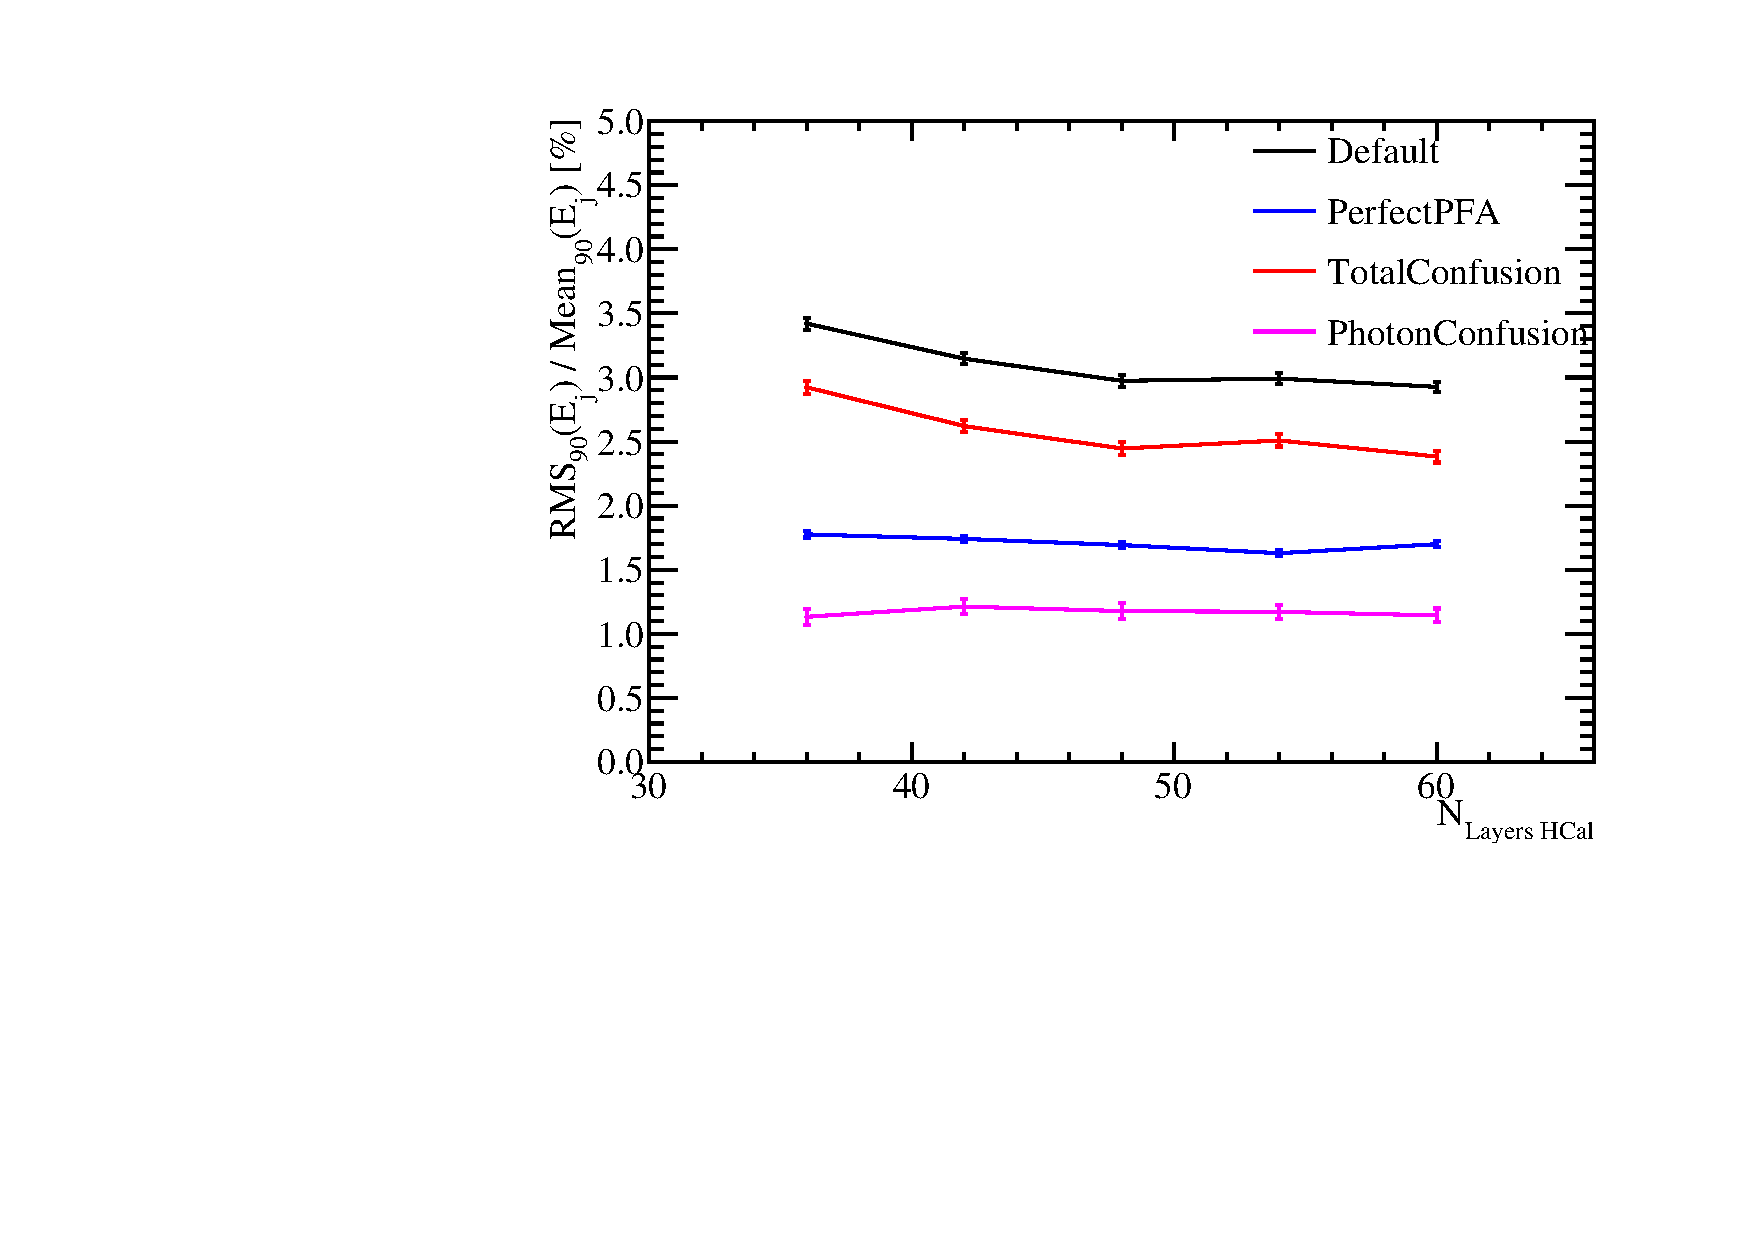
\includegraphics[width=0.5\textwidth]{OptimisationStudies/Plots/JetEnergyResolutions/JER_vs_NumberOfHCalLayersOfFixedDepth_500GeV_DiJet_Breakdown.pdf}}
\caption[The contributions to the jet energy resolution as a function of number of layers in the HCal using the nominal ILD detector model for \protect\subref{fig:hcalnfixedlayers45break} 45~GeV jets and \protect\subref{fig:hcalnfixedlayers250break} 250~GeV jets.  The black curves correspond to the standard reconstruction, the blue curves to the intrinsic energy resolution contribution to the jet energy resolution, the red curves to the confusion contribution to the jet energy resolution and the magenta curves to the confusion contribution to the jet energy resolution related solely to $\gamma$ reconstruction.]{The contributions to the jet energy resolution as a function of number of layers in the HCal using the nominal ILD detector model for \protect\subref{fig:hcalnfixedlayers45break} 45~GeV jets and \protect\subref{fig:hcalnfixedlayers250break} 250~GeV jets.  The black curves correspond to the standard reconstruction, the blue curves to the intrinsic energy resolution contribution to the jet energy resolution, the red curves to the confusion contribution to the jet energy resolution and the magenta curves to the confusion contribution to the jet energy resolution related solely to $\gamma$ reconstruction.}
\label{fig:hcalnfixedlayersbreak}
\end{figure}

In summary, even if the number of layers in the HCal were reduced by a factor of 25\% the jet energy resolution would be sufficient for separating the hadronic decays of the W and Z bosons at ILC energies.  However, it is clear that leakage of energy from the back of the HCal would negatively affect events at ILC like energies if the number of layers is reduced from the nominal value of 48 layers, therefore, it is desirable to have a minimum of 48 layers in the HCal.
  
%========================================================================================

\subsection{HCal Sampling Frequency}
\label{sec:hcalsamplingfrequency}
Several detector models were simulated where the sampling frequency in the HCal had been modified from that found in the nominal ILD HCal.  This sampling fraction was altered by changing the number of layers in the HCal, while simultaneously changing the active and absorber layer thicknesses, to maintain the total depth of the HCal, in $\lambda_{I}$.  For each model considered, the absorber material was steel, containing a total of 5.72~$\lambda_{I}$, and the active material was scintillator, containing a total of 0.19~$\lambda_{I}$.  The ratio of the active to absorber layers thicknesses (the sampling fraction) in these models matched that found in the nominal ILD HCal.  A summary of the detector models considered in this study can be found in table \ref{table:nlayershcaloption}.  

\begin{table}[h!]
\centering
\begin{tabular}{ l l l }
\hline
Number $N_{\text{Layers HCal}}$& Absorber Thickness & Active Thickness \\
 & [mm] & [mm] \\
\hline
60 & 16.00 & 2.40 \\ 
54 & 17.78 & 2.67 \\
48 & 20.00 & 3.00 \\
42 & 22.86 & 3.43 \\
36 & 26.67 & 4.00 \\
30 & 32.00 & 4.80 \\
24 & 40.00 & 6.00 \\
18 & 53.33 & 8.00 \\
\hline
\end{tabular}
\caption[Cell size layout of various HCal models considered.]{Cell size layout of various HCal models considered.}
\label{table:nlayershcaloption}
\end{table}

Increasing the number of layers in a sampling calorimeter, while leaving the total material budget unchanged, will lead to greater sampling of particles showering within it and a reduction the stochastic contribution to the energy resolution.  Therefore, it is expected that the energy resolution will improve with increasing number of layers in the HCal.  This is shown for 50~GeV $\text{K}^{0}_{L}$ in figure \ref{fig:hcalnlayerser}, which clearly shows that the energy resolution of the calorimeter is strongly dependent upon the sampling frequency in the HCal.  There are fluctuations in the energy resolution from fitting the reconstructed energy distribution to extract the mean and from the calibration of the detector, however, these are small and the underlying performance trend is still clear.  The energy resolution does not exactly follow a $\frac{1}{\sqrt{N_{\text{Readout Layers HCal}}}}$ relationship, but this is to be expected as this relationship only holds for the energy resolution of a single sampling calorimeter and these results are for the whole ILD detector, including the $\approx 1 \lambda_{I}$ in the ECal.  Furthermore, this functional form neglects the constant term in the energy resolution described in section \ref{sec:nominaldetectorperformance}.  

\begin{figure}[h!]
\centering
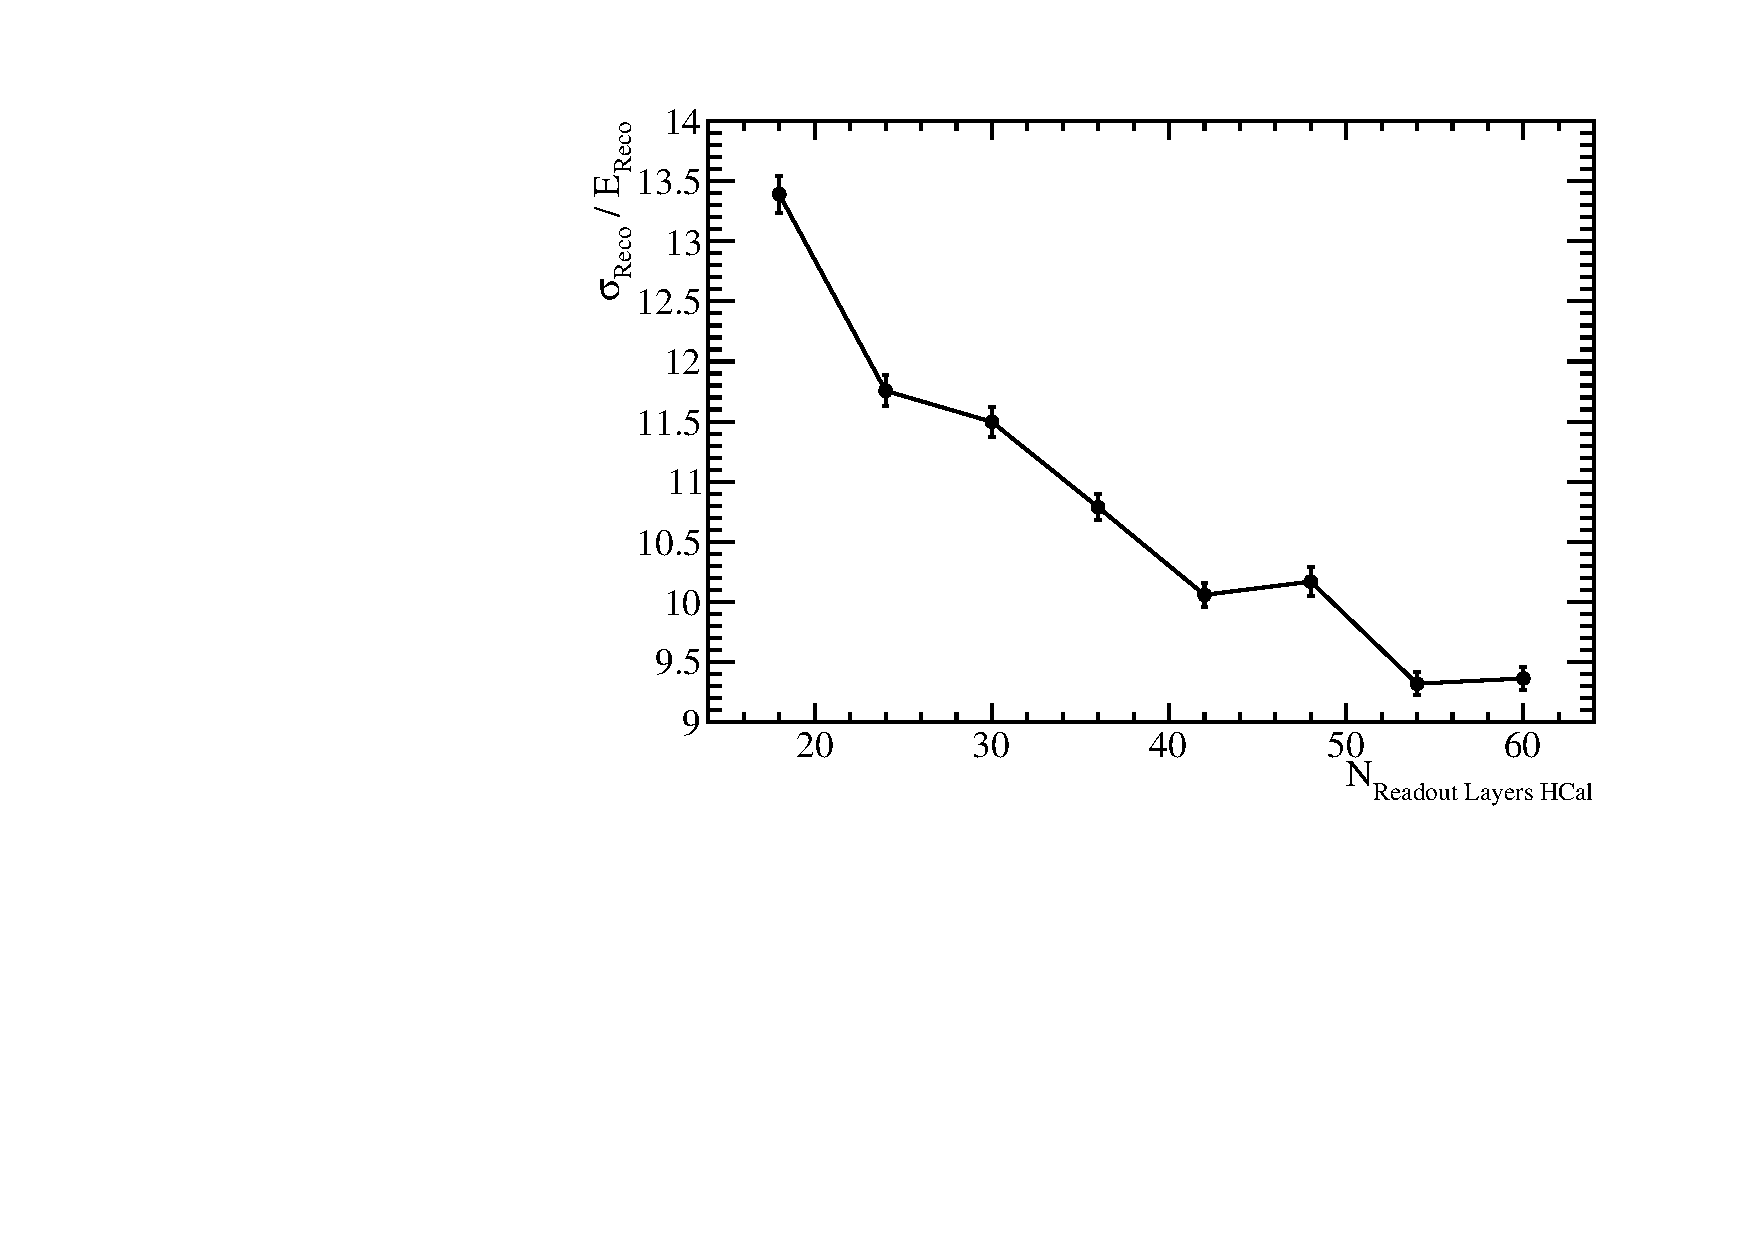
\includegraphics[width=0.5\textwidth]{OptimisationStudies/Plots/EnergyResolution/ER_vs_NHCalVariableLayers_50GeVKaon0L.pdf}
\caption[The energy resolution as a function of sampling frequency in the HCal for 50~GeV $\text{K}^{0}_{L}$ events using the nominal ILD detector model.]{The energy resolution as a function of sampling frequency in the HCal for 50~GeV $\text{K}^{0}_{L}$ events using the nominal ILD detector model.}
\label{fig:hcalnlayerser}
\end{figure}  

The jet energy resolution as a function of sampling frequency in the HCal is shown in figure \ref{ig:hcalnlayers}.  It is clear that increasing the number of layers in the HCal leads to an improvement in the jet energy resolution.  Figure \ref{fig:hcalnlayersbreak} shows that both the intrinsic energy resolution and confusion are reduced with increasing sampling frequency.  This is expected as increasing the sampling frequency of a calorimeter improves the intrinsic energy resolution, which has he knock-on effect of lowering the confusion contribution to the jet energy resolution as described in section \ref{sec:jerdecomposition}.   

\begin{figure}[h!]
\centering
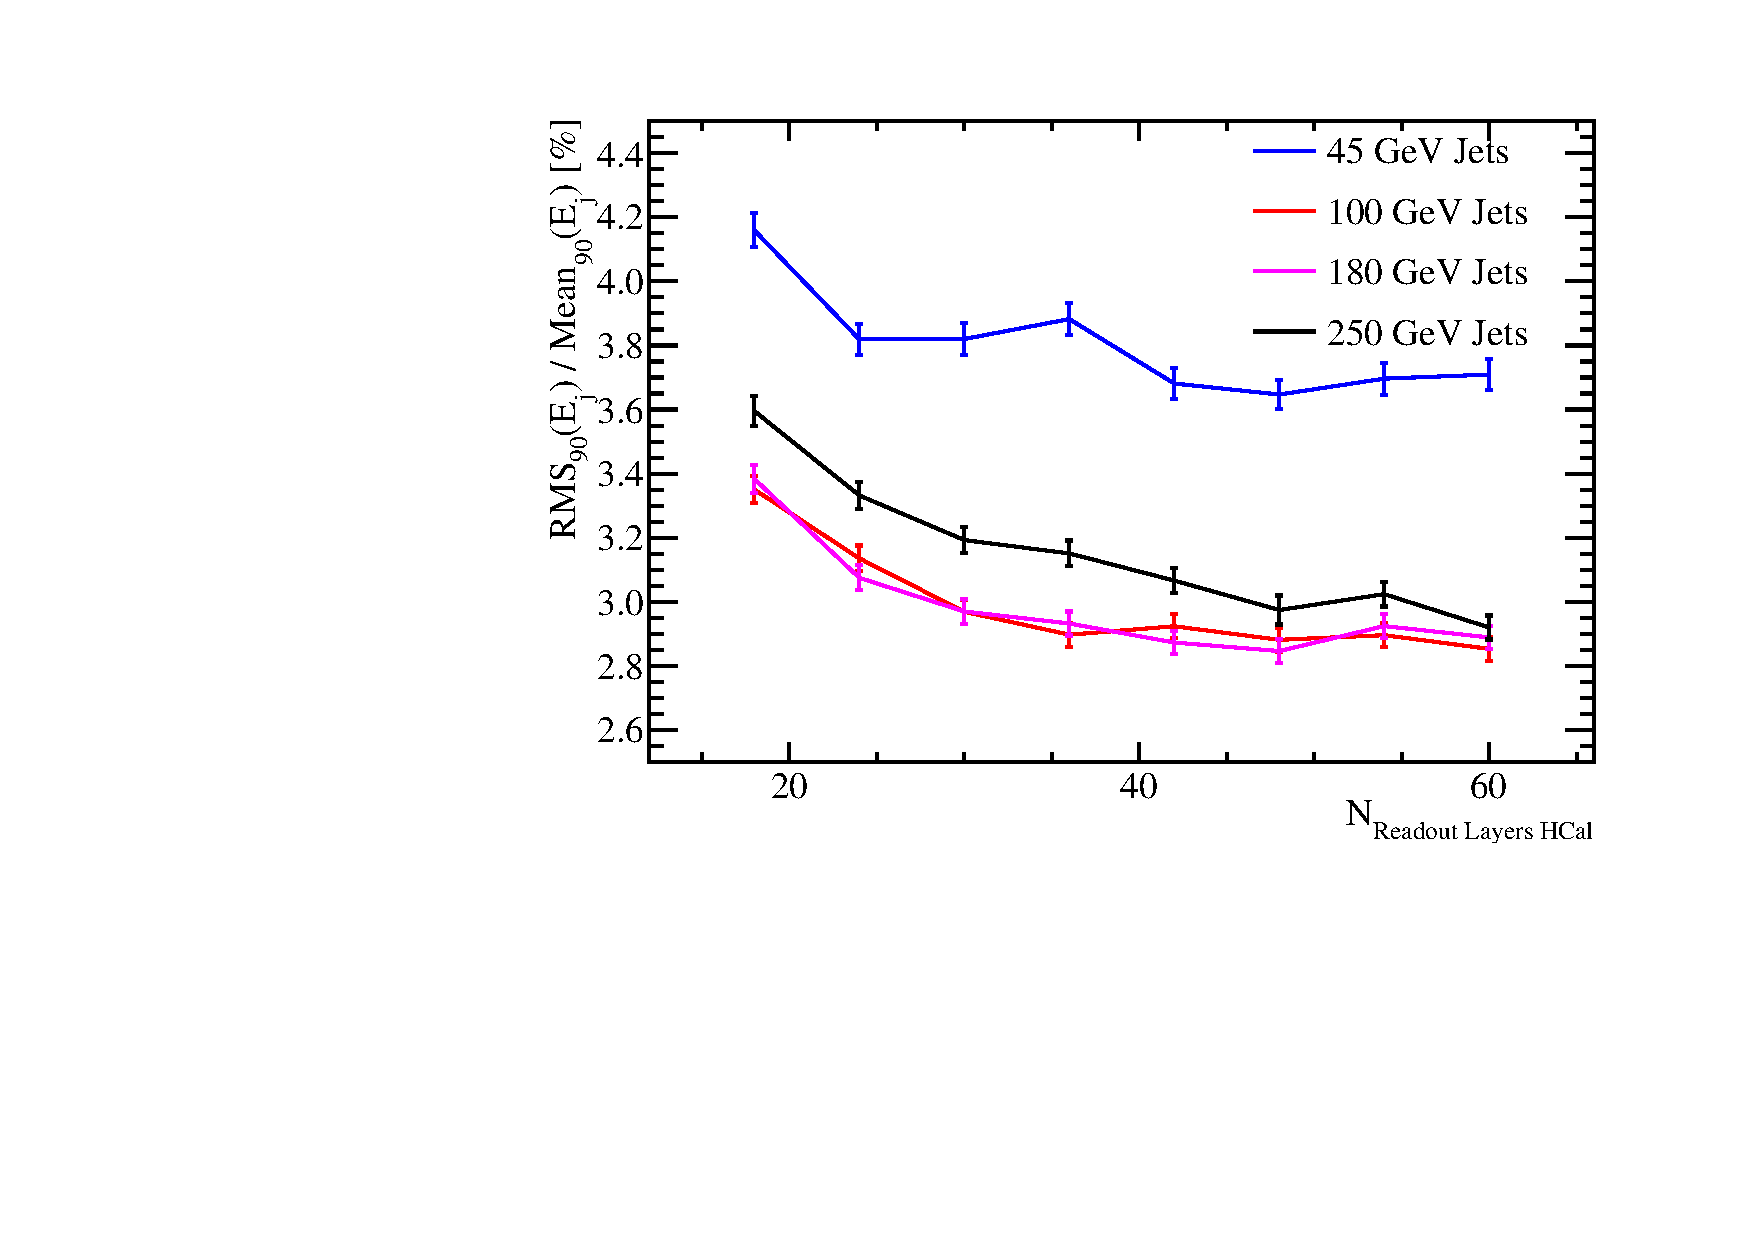
\includegraphics[width=0.5\textwidth]{OptimisationStudies/Plots/JetEnergyResolutions/JER_vs_NumberOfLayersInTheHCal.pdf}
\caption[The jet energy resolution as a function of sampling frequency in the HCal for various jet energies using the nominal ILD detector model.]{The jet energy resolution as a function of sampling frequency in the HCal for various jet energies using the nominal ILD detector model.}
\label{fig:hcalnlayers}
\end{figure}

\begin{figure}[h!]
\centering
\subfloat[]{\label{fig:hcalnlayers45break}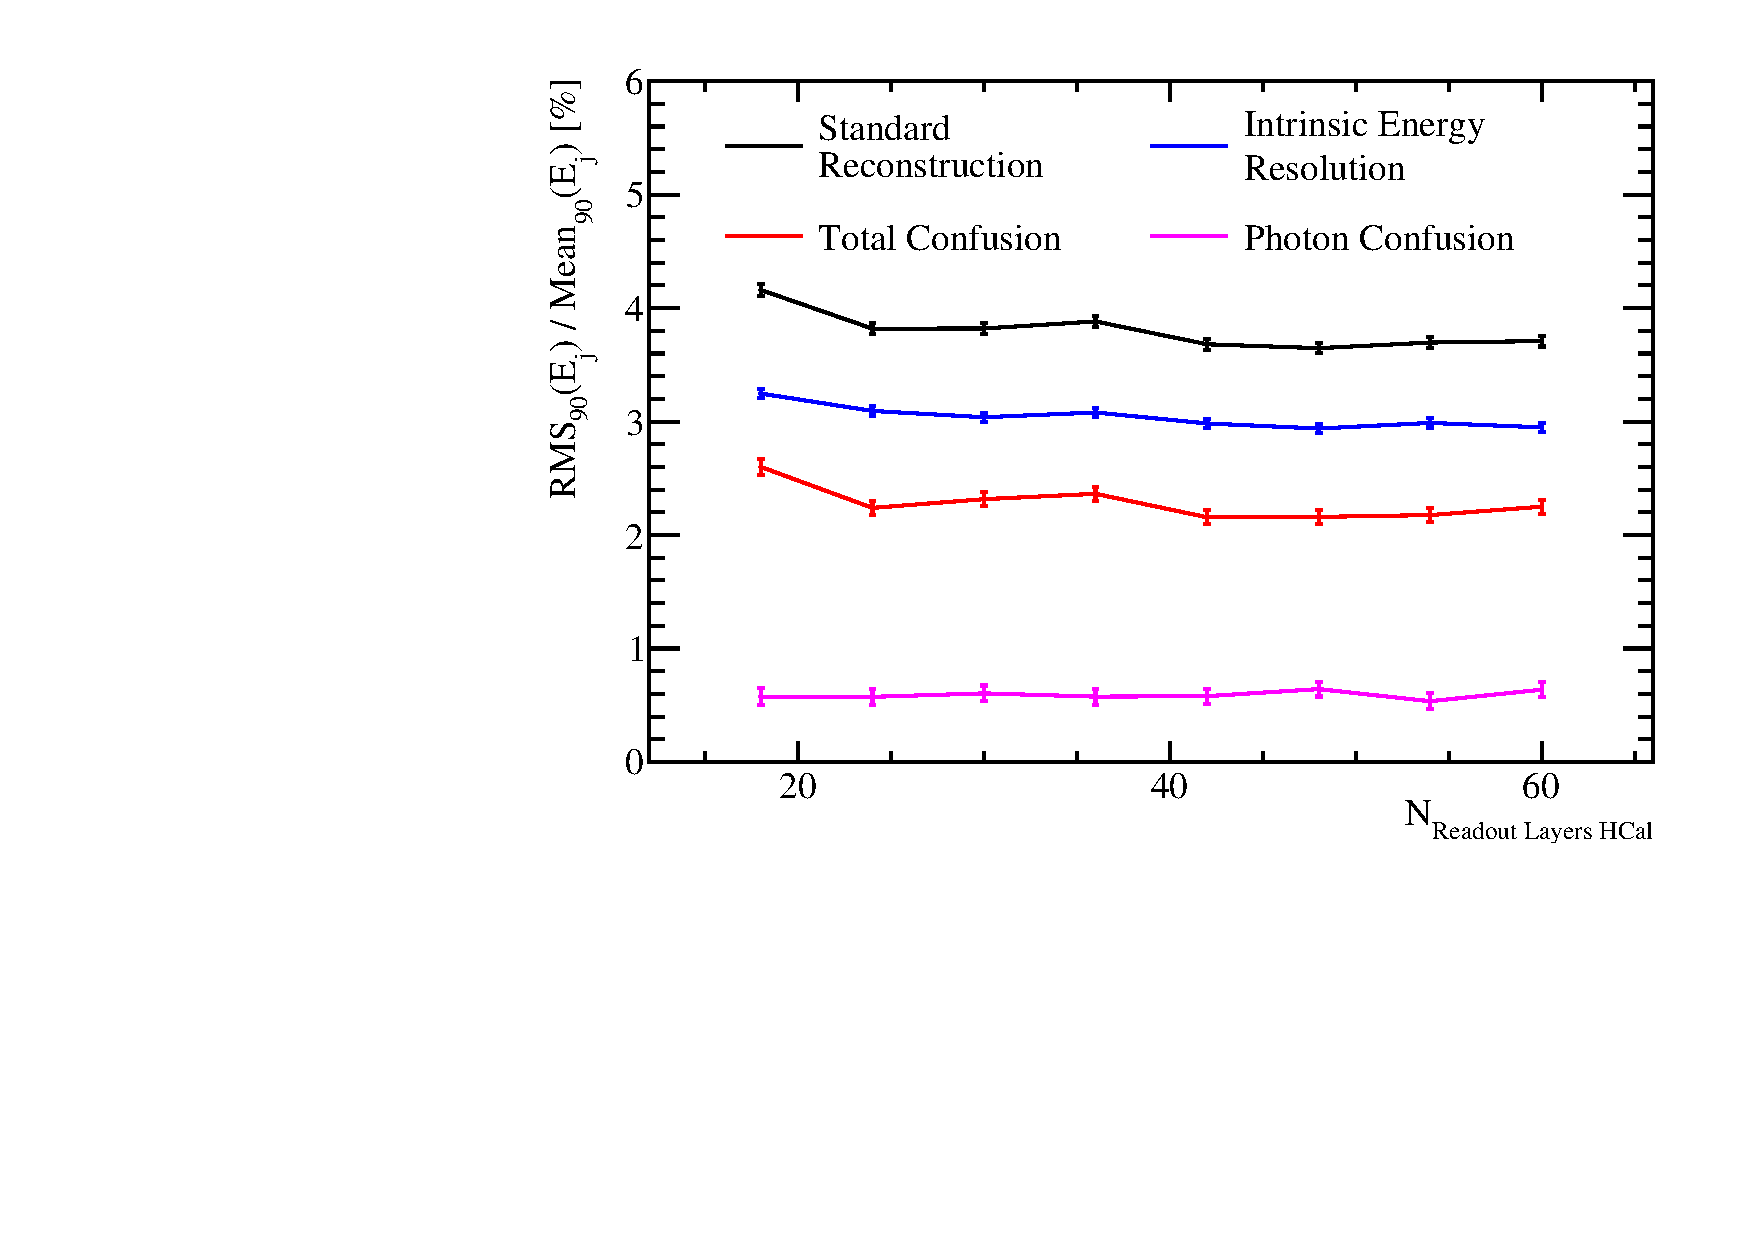
\includegraphics[width=0.5\textwidth]{OptimisationStudies/Plots/JetEnergyResolutions/JER_vs_NumberOfLayersInTheHCal_91GeV_DiJet_Breakdown.pdf}}
\subfloat[]{\label{fig:hcalnlayers250break}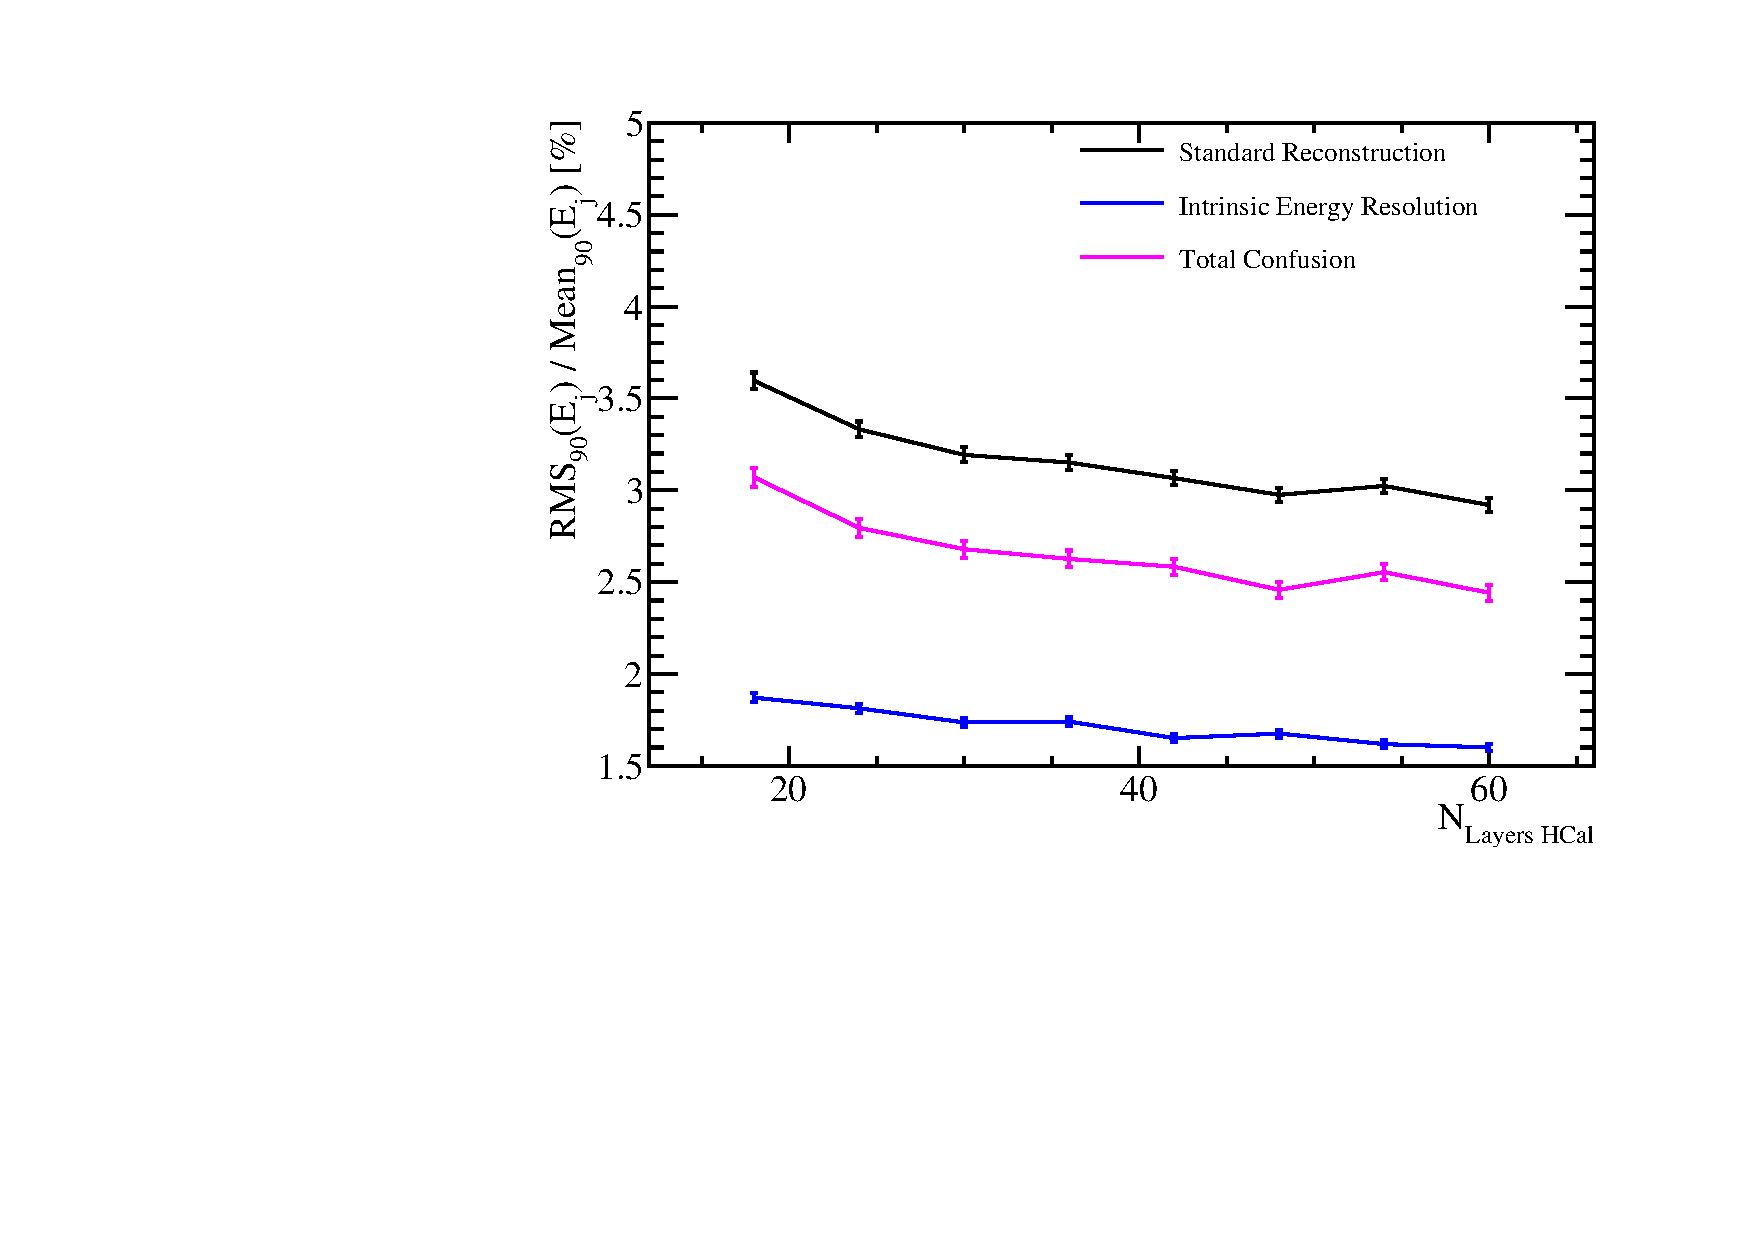
\includegraphics[width=0.5\textwidth]{OptimisationStudies/Plots/JetEnergyResolutions/JER_vs_NumberOfLayersInTheHCal_500GeV_DiJet_Breakdown.pdf}}
\caption[The contributions to the jet energy resolution as a function of sampling frequency in the HCal using the nominal ILD detector model for \protect\subref{fig:hcalnlayers45break} 45~GeV jets and \protect\subref{fig:hcalnlayers250break} 250~GeV jets.  The black curves correspond to the standard reconstruction, the blue curves to the intrinsic energy resolution contribution to the jet energy resolution, the red curves to the confusion contribution to the jet energy resolution and the magenta curves to the confusion contribution to the jet energy resolution related solely to $\gamma$ reconstruction.]{The contributions to the jet energy resolution as a function of sampling frequency in the HCal using the nominal ILD detector model for \protect\subref{fig:hcalnlayers45break} 45~GeV jets and \protect\subref{fig:hcalnlayers250break} 250~GeV jets.  The black curves correspond to the standard reconstruction, the blue curves to the intrinsic energy resolution contribution to the jet energy resolution, the red curves to the confusion contribution to the jet energy resolution and the magenta curves to the confusion contribution to the jet energy resolution related solely to $\gamma$ reconstruction.}
\label{fig:hcalnlayersbreak}
\end{figure}

It is clear that a larger number of layers in the HCal benefits both the intrinsic energy resolution of the ILD detector as well as reducing the confusion contribution to the jet energy resolution.  As there are few physics analyses that rely on the identification and categorisation of individual neutral hadrons, but there are many that rely on identification and categorisation of $\gamma$s, the intrinsic energy resolution of the HCal is less crucial from a physics perspective than that of the ECal.  However, these studies show the HCal still has a crucial role to play in jet reconstruction in the particle flow paradigm and therefore cannot be neglected.  To achieve a jet energy resolution of $\frac{\sigma_{E}}{E} \lesssim 3.8\%$, which is required to separate the W and Z hadronic decays, the ILD detector will require a minimum of 42 layers in the HCal.  This sampling frequency is required particularly for low energy jets where the energy resolution is dominated by the intrinsic energy resolution of the detector.

%========================================================================================

\subsection{HCal Sampling Fraction}
\label{sec:hcalsamplingfraction}
The ILD detector performance was simulated where the ratio of the active to absorber layer thicknesses in the HCal were varied.  In the nominal detector model the active scintillator layer thickness is 3 mm, while the absorber layer thickness is 20 mm giving a sampling fraction of 0.15.  HCal models were simulated where this ratio was changed from 0.05 to 0.25 in steps of 0.05, while retaining the same number of interaction lengths in the absorber and active layers as is found in the nominal HCal model.  If the active layer thickness becomes excessively small then it is possible that any signal produced in that layer would be insufficient to accurately estimate the energy deposited within the surrounding absorber layers.  However, no performance differences were observed for any of these detector models when considering the energy resolution for 50~GeV $\text{K}^{0}_{L}$ events or the jet energy resolution for the 91, 200, 360 and 500~GeV Z$\rightarrow$uds di-jet events.  This indicates the particle showers are sufficiently well sampled in all detector models considered and that thinning the active layer of the ILD HCal down to $\sim1$~mm would not harm the detector performance.  

%========================================================================================

\subsection{HCal Absorber Material}
\label{sec:hcalabsorbermaterial}
The nominal choice of absorber material is steel with tungsten providing a feasible alternative \cite{Blaising:2015nla}.  Although tungsten is more expensive than steel, it contains a larger number of nuclear interaction lengths per unit length.  Therefore, using tungsten as opposed to steel as the absorber material would allow for a reduction in the size of the HCal, while retaining the same number of nuclear interaction lengths.  Reducing the depth of the calorimeter would decrease the size of the solenoid required, which would offset some of the additional cost if tungsten were to be used. 

The configuration for the steel and tungsten HCal options that were used in the full ILD simulation can be found in table \ref{table:hcalabsmaterial}.  To isolate the effects of changing the absorber material, the total depth, in nuclear interaction lengths, was kept constant when comparing these two options.  Furthermore, the sampling fraction was also held constant.  The interaction of hadrons with the absorber material within the detector is simulated by GEANT4.  A number of different physics lists exist within GEANT4 for the modelling of hadronic showers.  The default model for high energy physics calorimetry is the QGSP\_BERT physics list, which uses the quark-gluon string model \cite{Folger:2003sb} with the precompound model of nuclear evaporation \cite{geantStringModel} (QGSP) for high energy interactions and the Bertini (BERT) cascade model \cite{Guthrie:1968ue} for intermediate energy interactions.  For this study both the QGSP\_BERT and the QGSP\_BERT\_HP physics lists were used.  The QGSP\_BERT\_HP list uses the high precision neutron package (NeutronHP) to deal with the transportation of neutrons from below 20 MeV to thermal energies.  This added detail was thought to be necessary for a study involving tungsten due to the expected increase in shower development.    

\begin{table}[h!]
\centering
\begin{tabular}{ l l l }
\hline
Parameter & Steel HCal Option & Tungsten HCal Option \\
\hline
Cell Size & $30 \times 30 \text{mm}^{2}$ square cells & $30 \times 30 \text{mm}^{2}$ square cells\\
Number of Layers & 48 readout layers & 48 readout layers\\
Absorber Material Thickness [mm] & 20.0 & 12.0 \\
Active Material Choice & Scintillator & Scintillator \\
Active Material Thickness [mm] & 3.0 & 1.8 \\
\hline
\end{tabular}
\caption[The configuration of the steel and tungsten HCal options.]{The configuration of the steel and tungsten HCal options.}
\label{table:hcalabsmaterial}
\end{table}

One of the dominant processes governing the energy deposition of hadronic showers in calorimeters is spallation \cite{Wigmans:2000vf}.  Spallation begins with the collision of a high energy incident particle with an atomic nuclei from the calorimeter absorbing material.  This collision creates an internuclear cascade where a shower of high energy hadronic particles, e.g. protons, neutrons and pions, are produced within the nucleus.  If these energies are large enough, some of these particles may escape the nucleus and form secondary particles in the hadronic shower.  After this initial collision, the nuclei of the absorbing material are left in an excited state.  Assuming the excited nuclei are sufficiently stable that they will not undergo fission, they will return to a stable state by ejecting energy in the form of particles in a process called evaporation.  Evaporation of neutrons, which is the dominant form of evaporation, significantly delays the growth of hadronic showers as after the evaporation process some of these neutrons participate in neutron capture \cite{Adloff:2014rya}.  Neutron capture involves an absorber nuclei capturing a neutron and then emitting a $\gamma$ as it returns to a stable state.  The time taken for the neutron capture mechanism to proceed is limited by the lifetime of the unstable nuclei, which typically makes neutron capture one of the slowest mechanisms by which hadronic showers can propagate.  As absorber materials with a large atomic number, Z, have a larger number of neutrons, it is expected that there will be an increase in the number of evaporation neutrons within hadronic showers developing in such materials.  In turn this will lead to more neutron capture processes and a longer development time for the hadronic showers.  This is what is observed when considering the shower development times using the tungsten (Z=74) and steel (iron, Z=26) HCal options as seen in figure \ref{fig:hcalabsmaterialtiming}. 

\begin{figure}[h!]
\centering
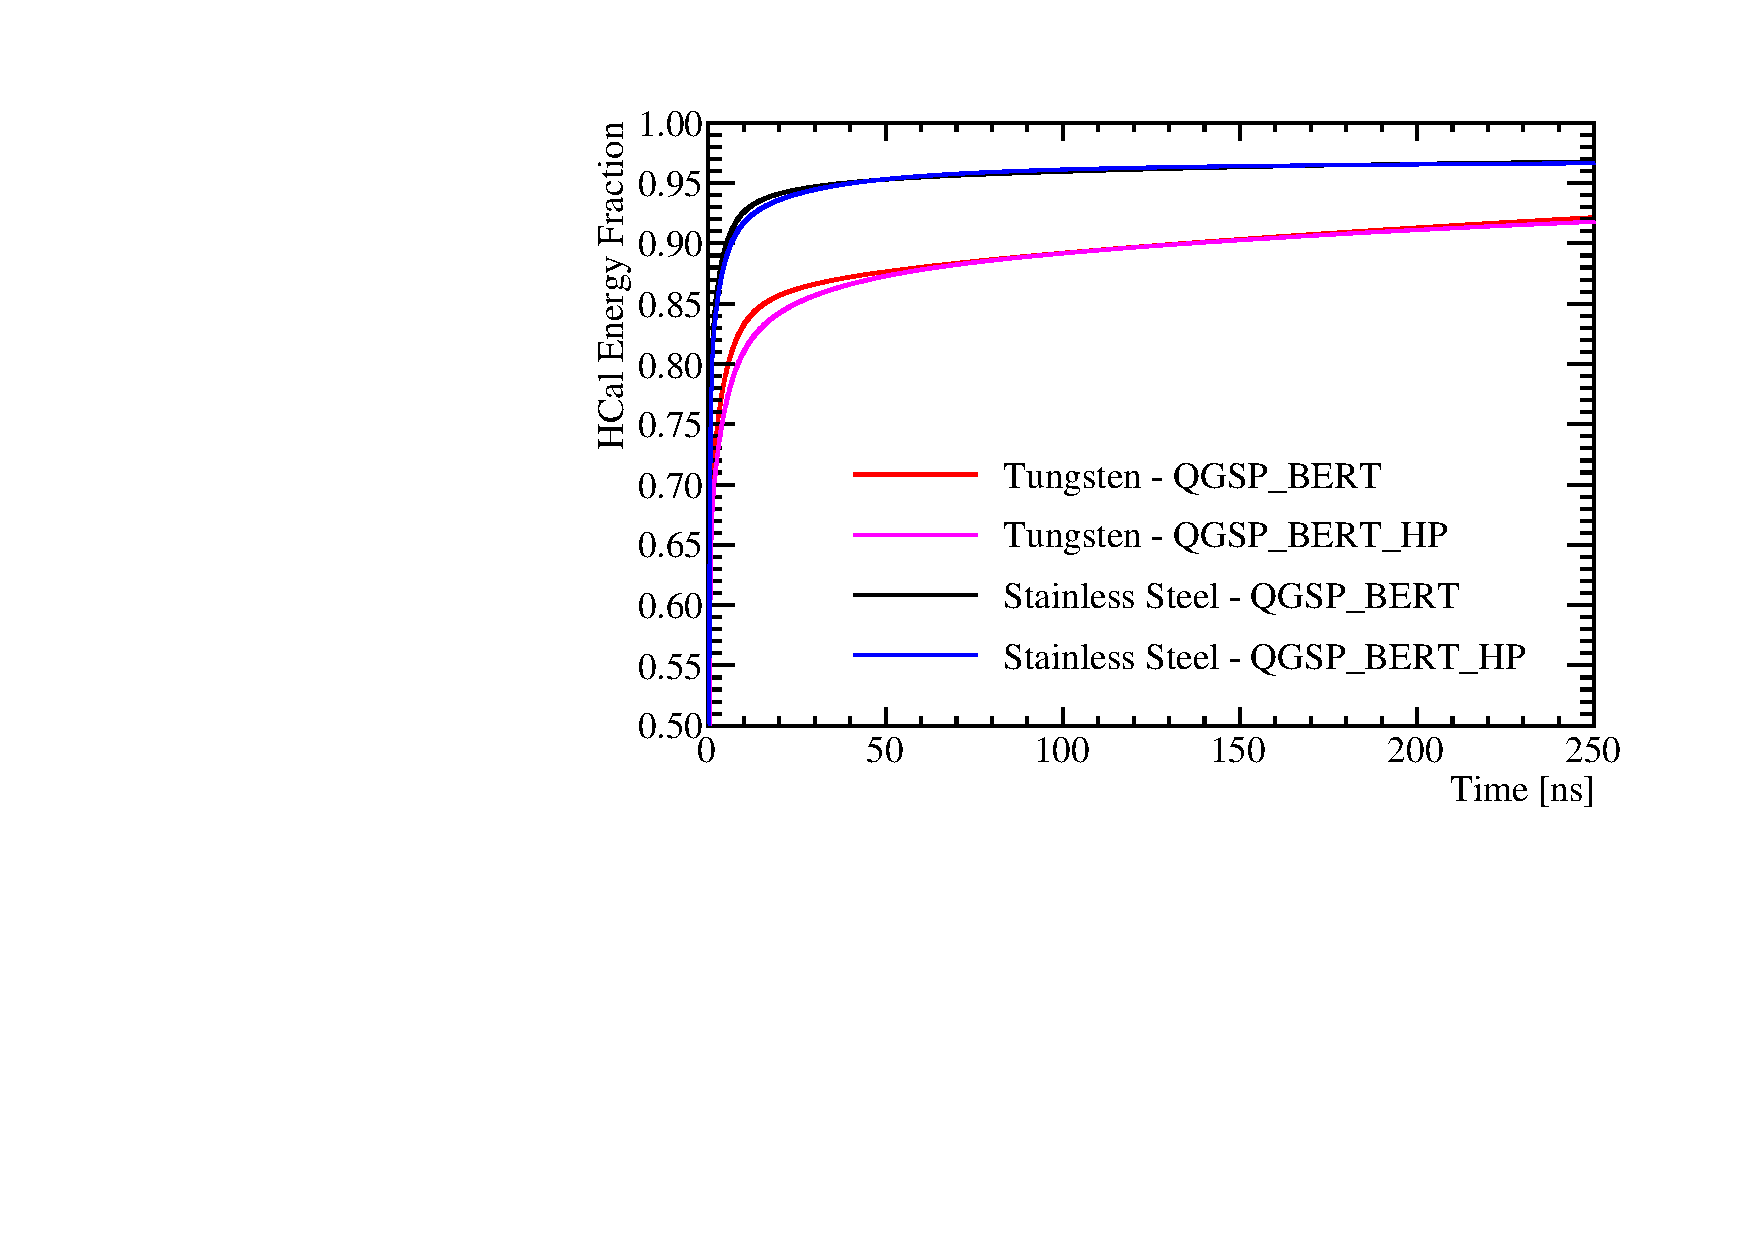
\includegraphics[width=0.5\textwidth]{OptimisationStudies/Plots/Description/HCalAbsorberMaterialTimings.pdf}
\caption[The fraction of the total calorimetric energy deposited in the HCal as a function of time for 25~GeV $\text{K}^{0}_{L}$ events using the steel and tungsten HCal options.  Results are shown for both the QGSP\_BERT and QGSP\_BERT\_HP physics lists.  The calorimeter hit times have been corrected for straight line time of flight to the impact point.]{The fraction of the total calorimetric energy deposited in the HCal as a function of time for 25~GeV $\text{K}^{0}_{L}$ events using the steel and tungsten HCal options.  Results are shown for both the QGSP\_BERT and QGSP\_BERT\_HP physics lists.  The calorimeter hit times have been corrected for straight line time of flight to the impact point.}
\label{fig:hcalabsmaterialtiming}
\end{figure} 

The energy resolution for 50~GeV $\text{K}^{0}_{L}$ events using the nominal ILD detector model with a steel and tungsten HCal absorber material can be found in table \ref{table:erhcalabsmaterial}.  The tungsten HCal option offers a slight improvement over steel in the energy resolution for these samples.  This will be caused by differences in the atomic structure of the two materials, which will lead to different developments of the hadronic showers within them. For example, the energy losses to nuclear binding energies are smaller in tungsten than steel, as the atomic nuclei for tungsten is less stable than that of iron, therefore, less energy is needed to liberate nucleons in the shower development.  This will lead to a larger signal in the tungsten calorimeter and a reduction in the energy resolution in comparison to steel.  These results also indicated that the addition of the high precision neutron package did not alter the detector performance significantly for either option.  

\begin{table}[h!]
\centering
\begin{tabular}{ l l l }
\hline
HCal Option & Energy Resolution [\%] \\
\hline
Steel, QGSP\_BERT & $8.8\pm0.2$ \\
Steel, QGSP\_BERT\_HP & $9.0\pm0.3$ \\
Tungsten, QGSP\_BERT & $8.3\pm0.2$ \\
Tungsten, QGSP\_BERT\_HP & $8.3\pm0.2$ \\
\hline
\end{tabular}
\caption[The energy resolution using the nominal ILD detector with various HCal options determined using 50~GeV $\text{K}^{0}_{L}$ events.]{The energy resolution using the nominal ILD detector with various HCal options determined using 50~GeV $\text{K}^{0}_{L}$ events.}
\label{table:erhcalabsmaterial}
\end{table}

It should be emphasised that in determining these results, the HCal cell truncation, as described in chapter \ref{chap:energyestimators}, was separately tuned for the tungsten option.  This was required as tungsten has a larger number of radiation lengths per unit length than steel, which leads to larger average cell energies meaning the truncation of cell energies required refining.  As the HCal primarily measures hadronic showers, one may naively expect the number of radiation lengths in the HCal to be irrelevant to performance, given both options have the same number of nuclear interaction lengths.  However, this is not the case as all hadronic showers have an electromagnetic component generated by the decays of hadrons to $\gamma$s, e.g  $\pi^{0} \rightarrow \gamma \gamma$ and $\eta \rightarrow \gamma \gamma$.  This leads to hadronic showers depositing more energy per calorimeter cell in a tungsten HCal when compared to a steel HCal.

The jet energy resolutions for selected jet energies are shown in table \ref{table:jerhcalabsmaterial} for the various HCal options considered.  These results indicate that steel outperforms tungsten as the absorber material for the HCal.  Furthermore, as the jet energy increases, the magnitude of the difference in jet energy resolutions between the two options grows.  This indicates the differences in jet energy resolution between the two options is driven by the confusion contribution as this contribution grows with increasing jet energy.  Furthermore, as the $\text{K}^{0}_{L}$ energy resolution was only slightly better for the tungsten option it is expected that the intrinsic energy resolution contribution to the jet energy resolution will not vary significantly between the two as only a small fraction of jet energy is measured in the HCal.  The intrinsic energy resolution and confusion contributions to the jet energy resolution for 45 and 250~GeV jets are shown in table \ref{table:jerbdhcalabsmaterial}.  As expected, the intrinsic energy resolution contribution to the jet energy resolution is nearly identical between the various options.  The confusion contribution to the jet energy resolution is larger for the tungsten HCal option than for the steel HCal option.  This is due to the PandoraPFA algorithms being tuned for the nominal (steel) ILD HCal dimensions, while the cells for the alternative tungsten option are thinner by a factor of approximately $\frac{\lambda_{I}^{Steel}}{\lambda_{I}^{Tungsten}} \approx 1.7$, where $\lambda_{I}^{x}$ is the distance of one radiation length in material $x$.  It is unfeasible to tune all of the PandoraPFA algorithms to each detector geometry, however, the breakdowns of the jet energy resolution indicate that even if this were done, the tungsten option would offer no advantage to the steel option in terms of intrinsic energy resolution.  Once again, it was noted that the use of the QGSP\_BERT\_HP physics list, as opposed to QGSP\_BERT, made a minimal impact on these results.

\begin{table}[h!]
\centering
\begin{tabular}{ l l l l l }
\hline
HCal Option & Jet Energy & & & \\
 & Resolution & & & \\
 & [\%] & & & \\
 & 45~GeV & 100~GeV & 180~GeV & 250~GeV \\
\hline
Steel, QGSP\_BERT & $3.65 \pm 0.05$ &$2.88 \pm 0.04$ &$2.85 \pm 0.04$ &$2.97 \pm 0.05$ \\
Steel, QGSP\_BERT\_HP & $3.67 \pm 0.05$ &$2.92 \pm 0.04$ &$2.86 \pm 0.04$ &$3.03 \pm 0.04$ \\
Tungsten, QGSP\_BERT & $3.78 \pm 0.05$ & $3.12 \pm 0.04$ & $3.15 \pm 0.04$ & $3.43 \pm 0.04 |$ \\
Tungsten, QGSP\_BERT\_HP & $3.80 \pm 0.05$ & $3.08 \pm 0.04$ & $3.24 \pm 0.04$ & $3.41 \pm 0.04$ \\
%Tungsten, QGSP\_BERT & $3.67 \pm 0.05$ &$3.12 \pm 0.04$ &$3.36 \pm 0.04$ &$3.76 \pm 0.05$ \\ 1~GeV Truncation 
%Tungsten, QGSP\_BERT\_HP & $3.69 \pm 0.05$ &$3.03 \pm 0.04$ &$3.38 \pm 0.04$ &$3.80 \pm 0.05$ \\ 1~GeV Truncation
\hline
\end{tabular}
\caption[The jet energy resolution using the nominal ILD detector with various HCal options for various jet energies.]{The jet energy resolution using the nominal ILD detector with various HCal options for various jet energies.}
\label{table:jerhcalabsmaterial}
\end{table}

\begin{table}[h!]
\centering
\begin{tabular}{ l l l l l }
\hline
HCal Option & Jet Energy & & & \\
 & Resolution & & & \\
 & [\%] & & & \\
 & 45~GeV & & 250~GeV & \\
 & Intrinsic & Confusion & Intrinsic & Confusion \\
\hline
Steel, QGSP\_BERT & $2.93 \pm 0.04$ & $2.16 \pm 0.06$ & $1.69 \pm 0.02$ &$2.45 \pm 0.05$ \\
Steel, QGSP\_BERT\_HP & $2.98 \pm 0.04$ &$2.15 \pm 0.06$ &$1.65 \pm 0.02$ &$2.53 \pm 0.04$ \\
Tungsten, QGSP\_BERT & $2.97 \pm 0.04$ & $2.34 \pm 0.06$ & $1.65 \pm 0.02$ & $3.01 \pm 0.05$ \\
Tungsten, QGSP\_BERT\_HP & $2.92 \pm 0.04$ & $2.42 \pm 0.06$ & $1.65 \pm 0.02$ & $2.99 \pm 0.05$ \\
\hline
\end{tabular}
\caption[The contributions to the jet energy resolution using the nominal ILD detector with various HCal options for 45 and 250~GeV jet energies.]{The contributions to the jet energy resolution using the nominal ILD detector with various HCal options for 45 and 250~GeV jet energies.}
\label{table:jerbdhcalabsmaterial}
\end{table}

In conclusion, there are no large differences in the intrinsic energy resolution of the ILD detector simulation, for either neutral hadrons or jets, when changing the HCal absorber material from steel to tungsten.  The steel option HCal outperforms the tungsten option in terms of pattern recognition confusion, when using the default PandoraPFA settings, although this could be addressed should it become clear that tungsten were a preferred option.  However, when examining the mechanical properties of steel and tungsten, it is clear that steel has a significant advantage over tungsten in terms of rigidity \cite{Linssen:2012hp}.  This means that fewer support structures would be required for the calorimeter leading to less dead material and better performance, which makes steel the more preferred option of the two.

%========================================================================================
%========================================================================================

\section{Global Detector Parameters}
The detector geometry and the magnetic field strength are major cost drivers for the ILD detector.  Both will have an affect on the jet energy resolution and, for completeness, studies showing their impact on detector performance are presented here.

%========================================================================================

\subsection{The Magnetic Field Strength}
\label{sec:bfield}
In the particle flow paradigm the momentum of charged particles is obtained through the curvature of the track they traverse as they bend in the magnetic field.  Therefore, the magnetic field is an integral element for the successful application of particle flow calorimetry.  Furthermore, the magnetic field deflects charged particles away from neutral particles in jets.  The stronger the magnetic field, the larger the separation between the calorimetric energy deposits made by charged and neutral particles in jets, which reduces the effect of confusion.  Therefore, it is expected that a stronger magnetic field will lead to better jet energy resolutions through a reduction of the confusion contribution to the jet energy resolution.  

Detector models were simulated where the magnetic field was varied from 1 to 5~T in steps of 0.5~T and the jet energy resolutions for these detectors is shown in figure \ref{fig:bfield}.  For high energy jets there is a strong trend whereby a stronger magnetic field leads to a better jet energy resolution.  While, at low jet energies the jet energy resolution is almost invariant to changes in the magnetic field.  

\begin{figure}[h!]
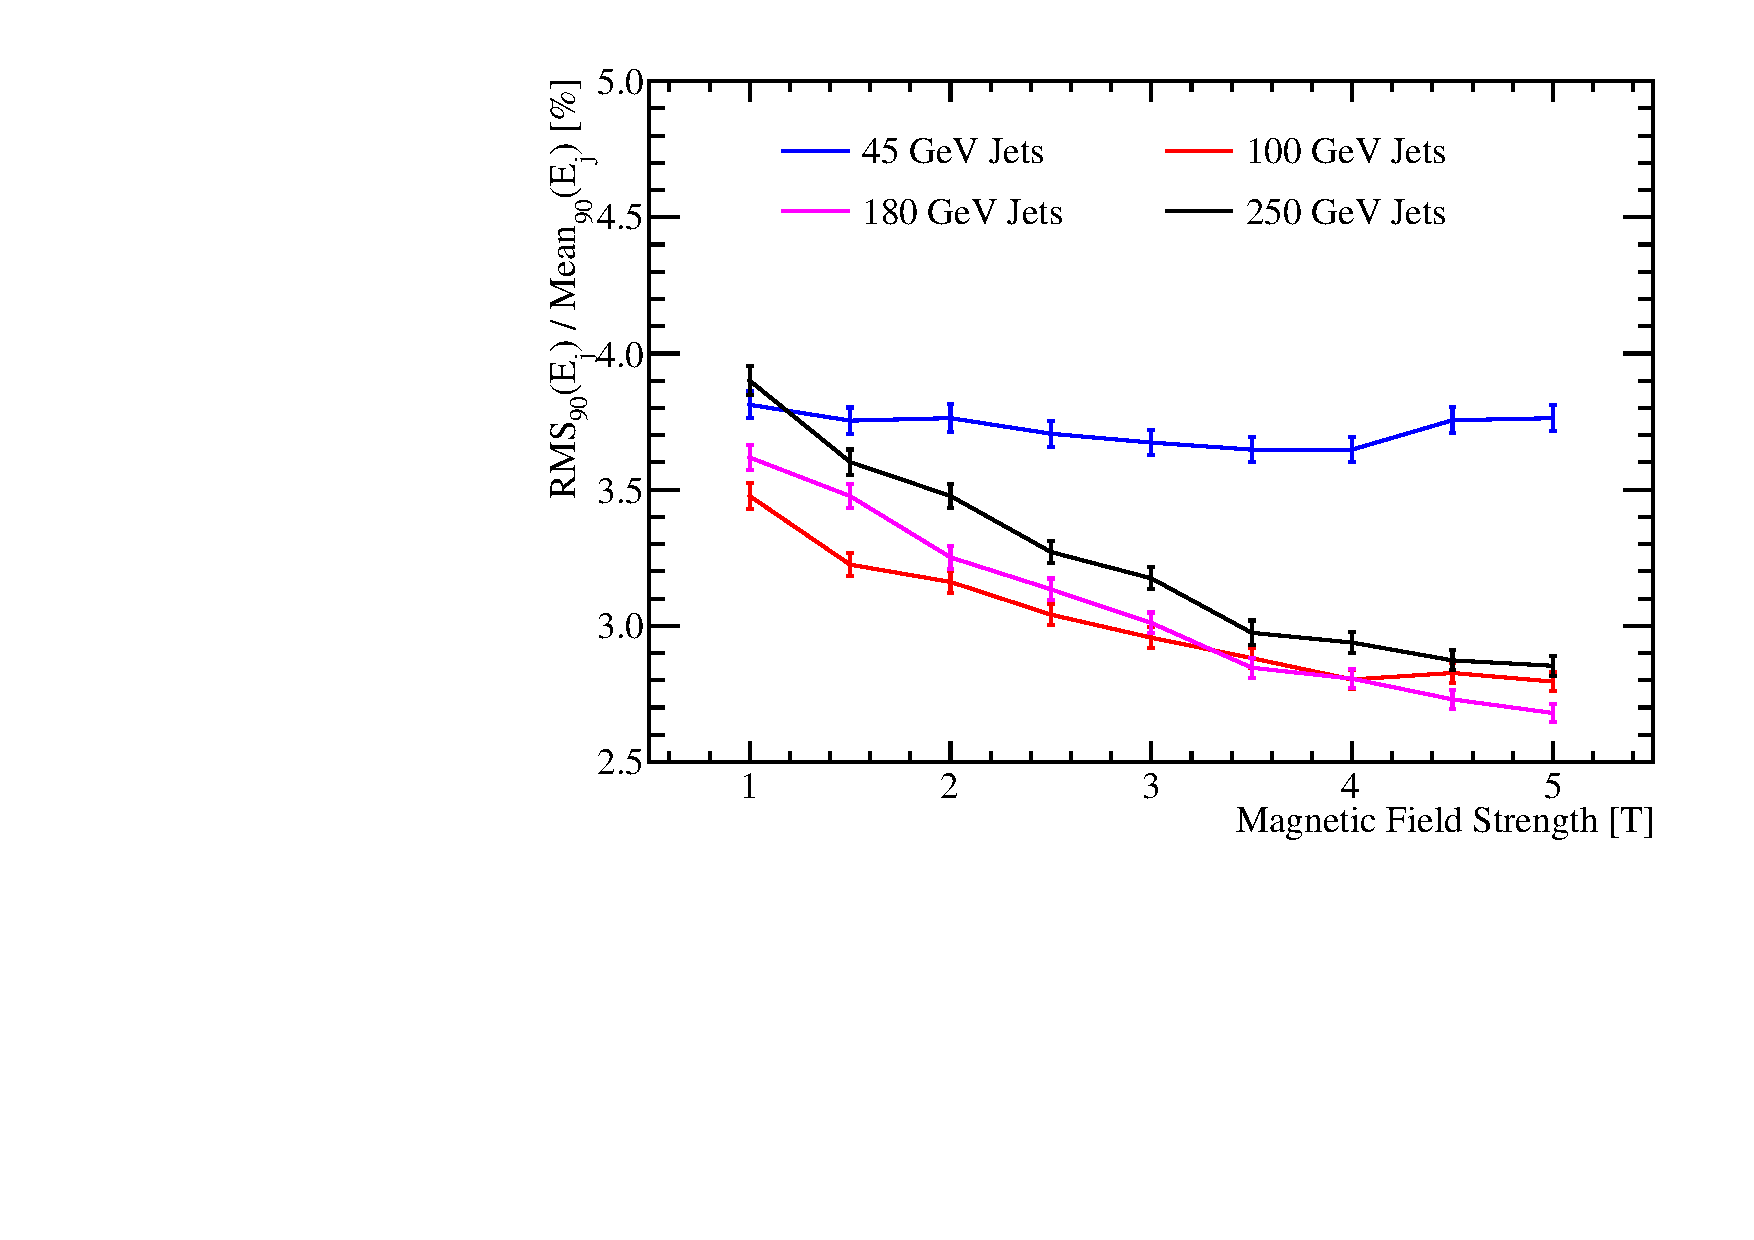
\includegraphics[width=0.5\textwidth]{OptimisationStudies/Plots/JetEnergyResolutions/JER_vs_MagneticFieldStrength.pdf}
\caption[The jet energy resolution using the nominal ILD detector as a function of the magnetic field strength for various jet energies.]{The jet energy resolution using the nominal ILD detector as a function of the magnetic field strength for various jet energies.}
\label{fig:bfield}
\end{figure}

The jet energy resolution breakdowns into the various contributions are shown in figure \ref{fig:bfieldbreak} and as expected there is clear reduction in the confusion contribution to the jet energy resolution with increasing magnetic field strength.  Furthermore, there is a reduction in intrinsic energy resolution with increasing magnetic field strength for low energy jets.  At low energies, the radius of curvature of the helix charged particles traverse will be small.  If the radius for a given particle is small enough, the particle will not enter the calorimeters.  In this case, only if the track produced from this particle passes tight selection cuts, designed to ensure the track originates from the IP, will the track be used in the reconstruction.  Therefore, energy can and will be lost from events where particles are stuck within the tracker.  Given the radii of curvature is inversely proportional to the magnetic field strength, the larger the magnetic field strength the more tracks will be confined to the tracker as is shown by figure \ref{fig:bfieldchargedparticles}.  The more tracks that are confined to the tracker, the worse the intrinsic energy resolution becomes as inevitably some tracks fail the quality cuts.  At high jet energies, low transverse momentum charged particles will still get trapped within the tracker, however, these contribute fractionally little energy to the total reconstructed energy.  Therefore, the trend of worsening intrinsic energy resolution with increasing magnetic field strength is less pronounced as the jet energy grows.  At very low magnetic field strengths and high jet energies, the intrinsic energy resolution actually degrades, due to an artefact in the determination of the intrinsic energy resolution.  The intrinsic energy resolution is determined by associating a single MC particle to each calorimeter cell.  At low magnetic field strengths and high jet energies, many of the MC particles will have overlapping energy deposits within the calorimeter cells and so associating a single MC particle per cell is inaccurate.  This leads to imperfect association of charged particle tracks to calorimetric energy deposits, which worsens the intrinsic energy resolution.  However, as this effect is second order small in comparison to changes in the confusion contribution the overall dependancy of detector performance on the magnetic field strength can be confidently quantified.  

\begin{figure}[h!]
\subfloat[]{\label{fig:bfield45break}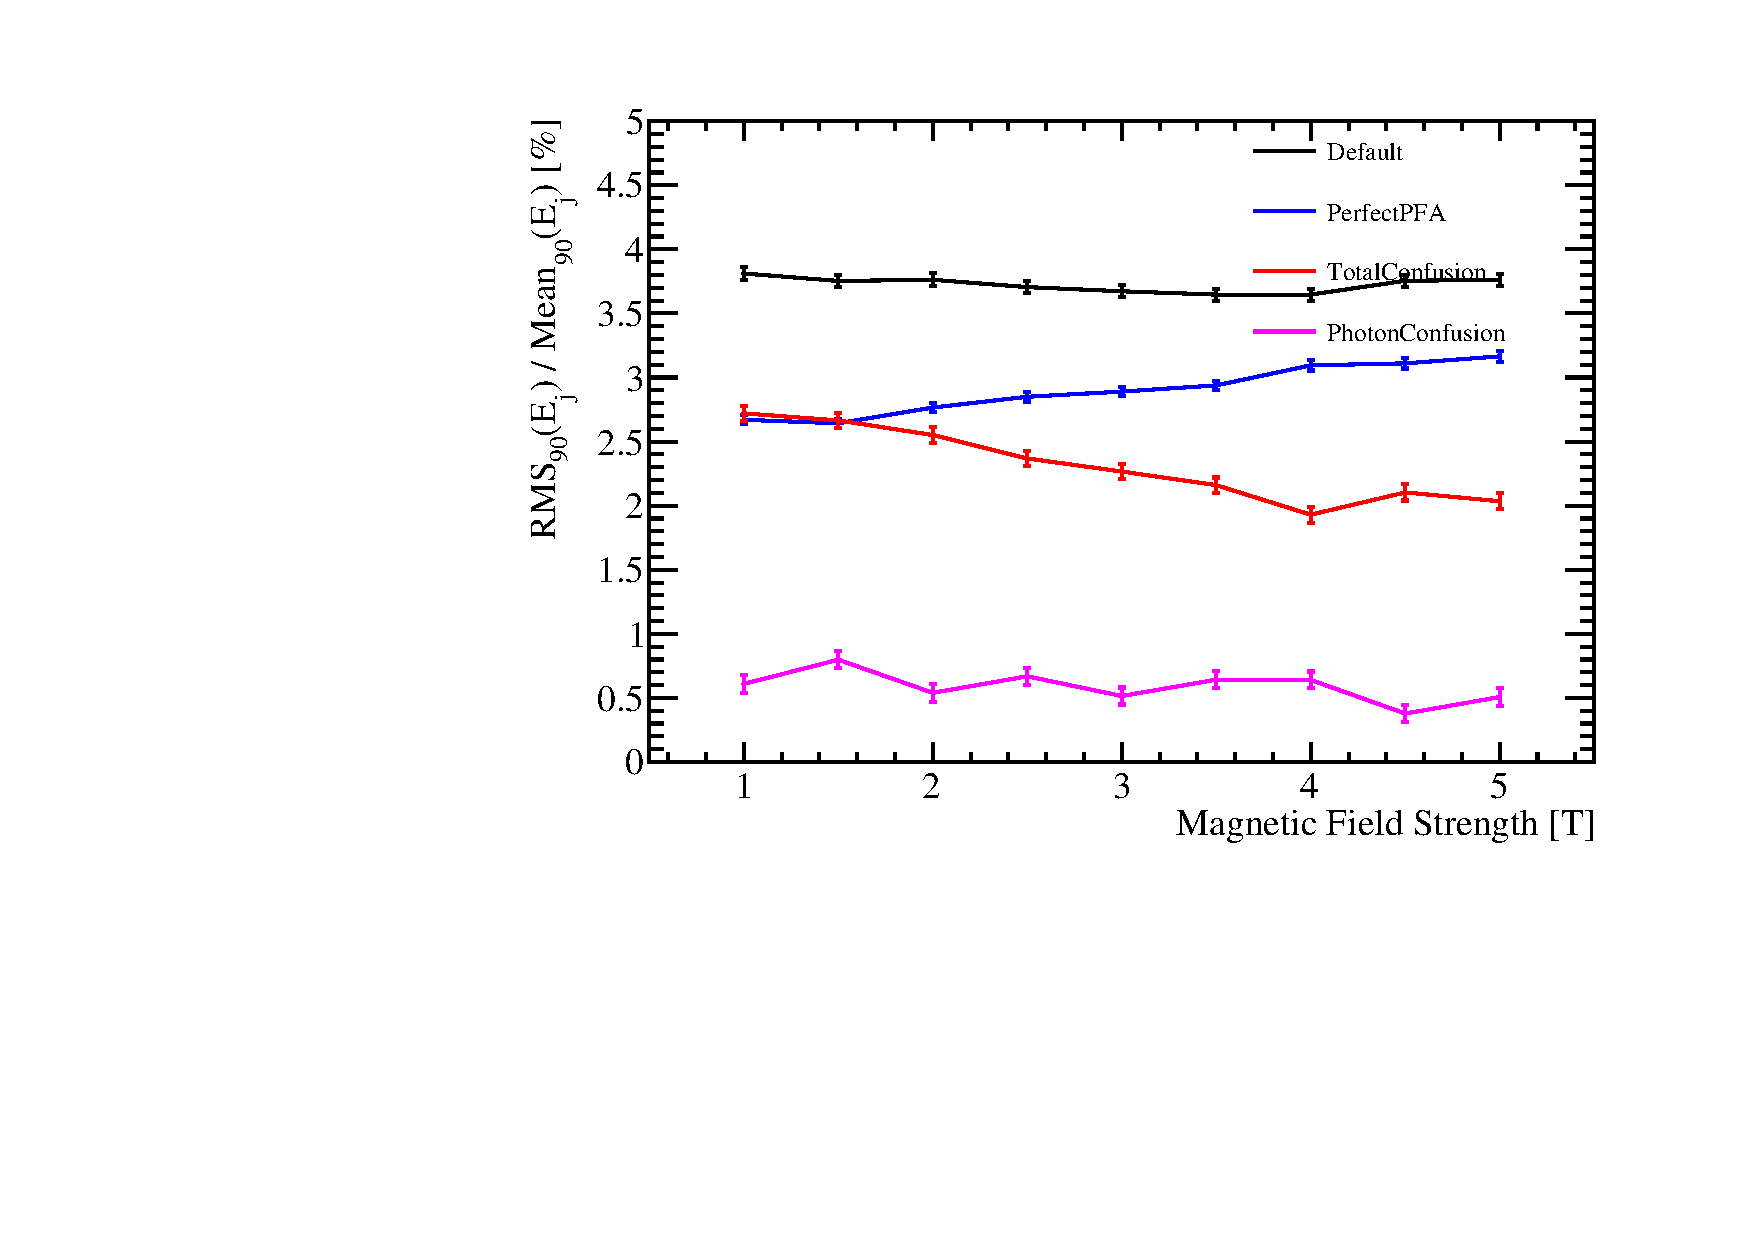
\includegraphics[width=0.5\textwidth]{OptimisationStudies/Plots/JetEnergyResolutions/JER_vs_MagneticFieldStrength_91GeV_DiJet_Breakdown.pdf}}
\subfloat[]{\label{fig:bfield250break}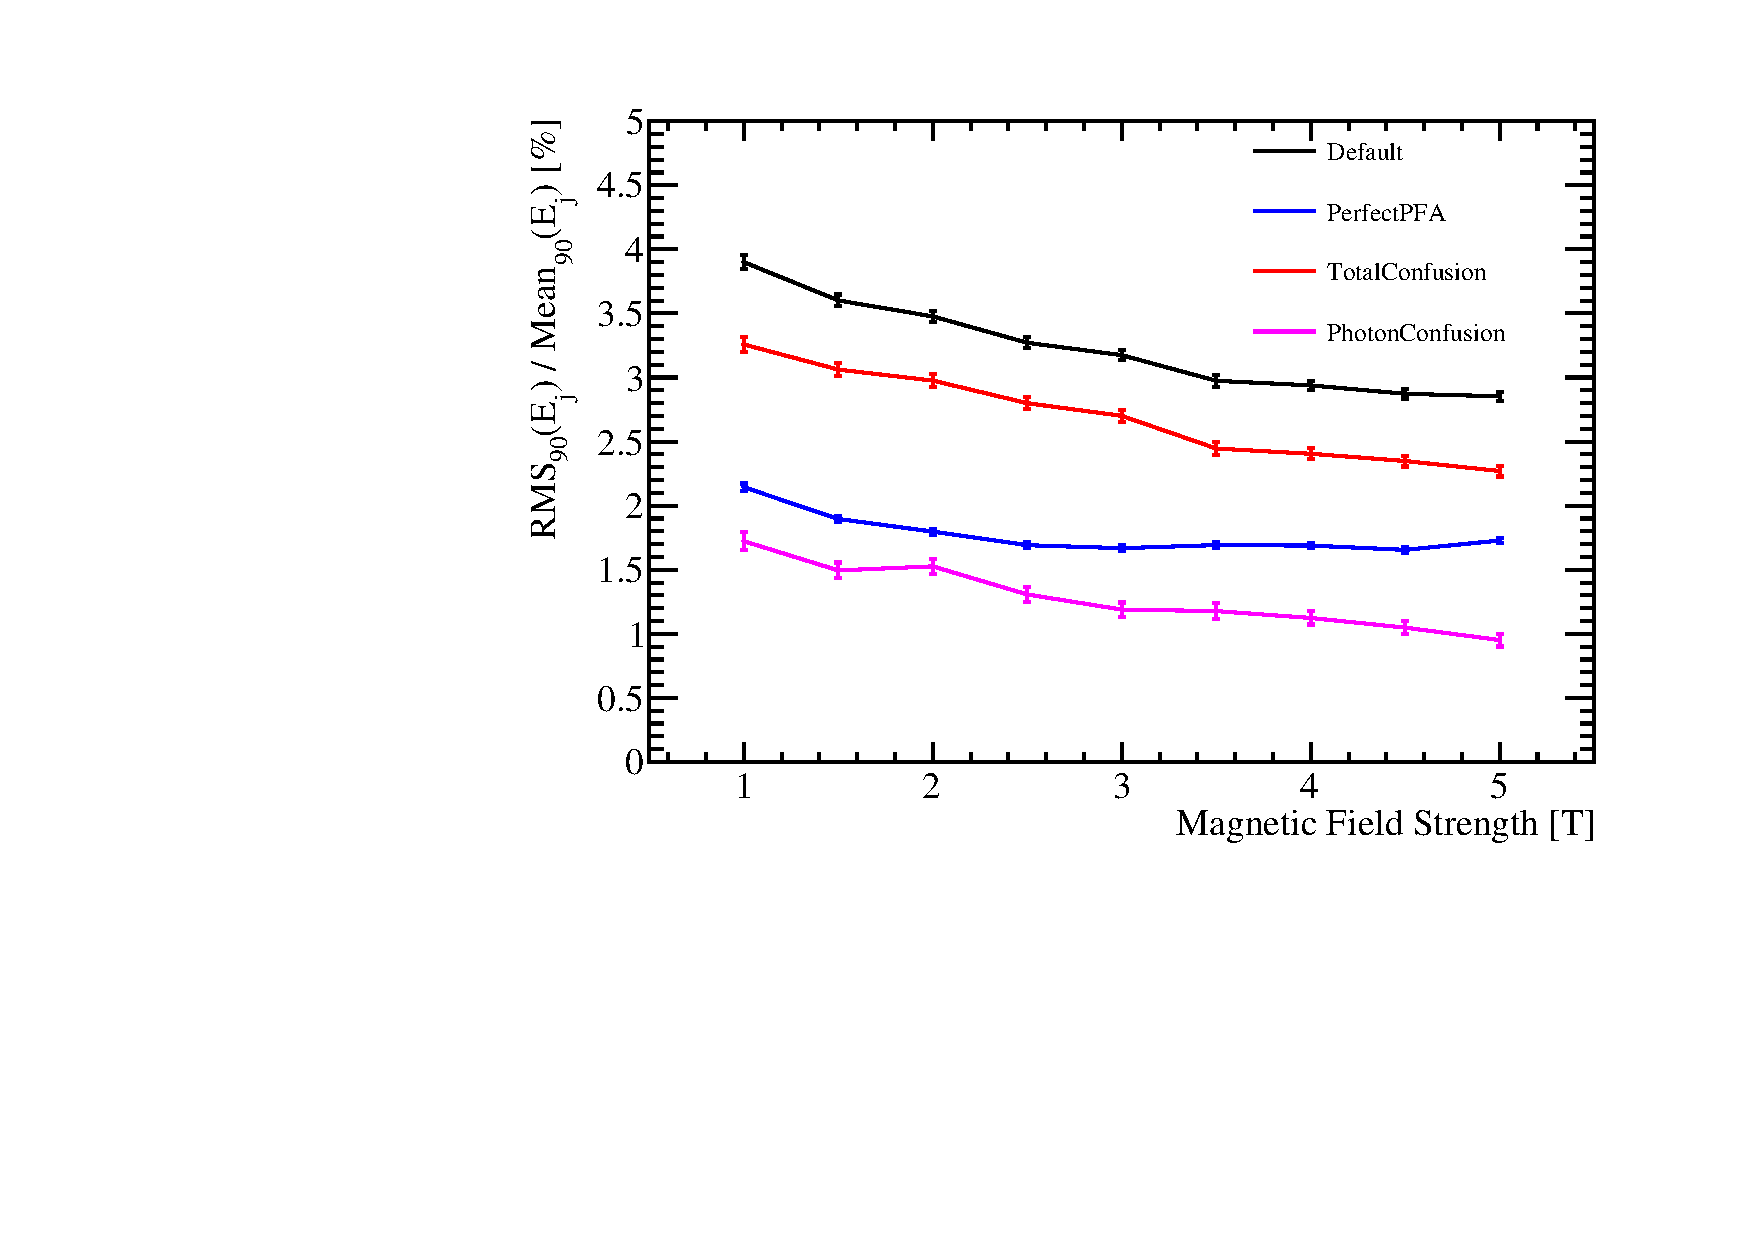
\includegraphics[width=0.5\textwidth]{OptimisationStudies/Plots/JetEnergyResolutions/JER_vs_MagneticFieldStrength_500GeV_DiJet_Breakdown.pdf}}
\caption[The contributions to the jet energy resolution as a function of the magnetic field strength using the nominal ILD detector model for \protect\subref{fig:bfield45break} 45~GeV jets and \protect\subref{fig:bfield250break} 250~GeV jets.  The black curves correspond to the standard reconstruction, the blue curves to the intrinsic energy resolution contribution to the jet energy resolution, the red curves to the confusion contribution to the jet energy resolution and the magenta curves to the confusion contribution to the jet energy resolution related solely to $\gamma$ reconstruction.]{The contributions to the jet energy resolution as a function of the magnetic field strength using the nominal ILD detector model for \protect\subref{fig:bfield45break} 45~GeV jets and \protect\subref{fig:bfield250break} 250~GeV jets.  The black curves correspond to the standard reconstruction, the blue curves to the intrinsic energy resolution contribution to the jet energy resolution, the red curves to the confusion contribution to the jet energy resolution and the magenta curves to the confusion contribution to the jet energy resolution related solely to $\gamma$ reconstruction.}
\label{fig:bfieldbreak}
\end{figure}

\begin{figure}[h!]
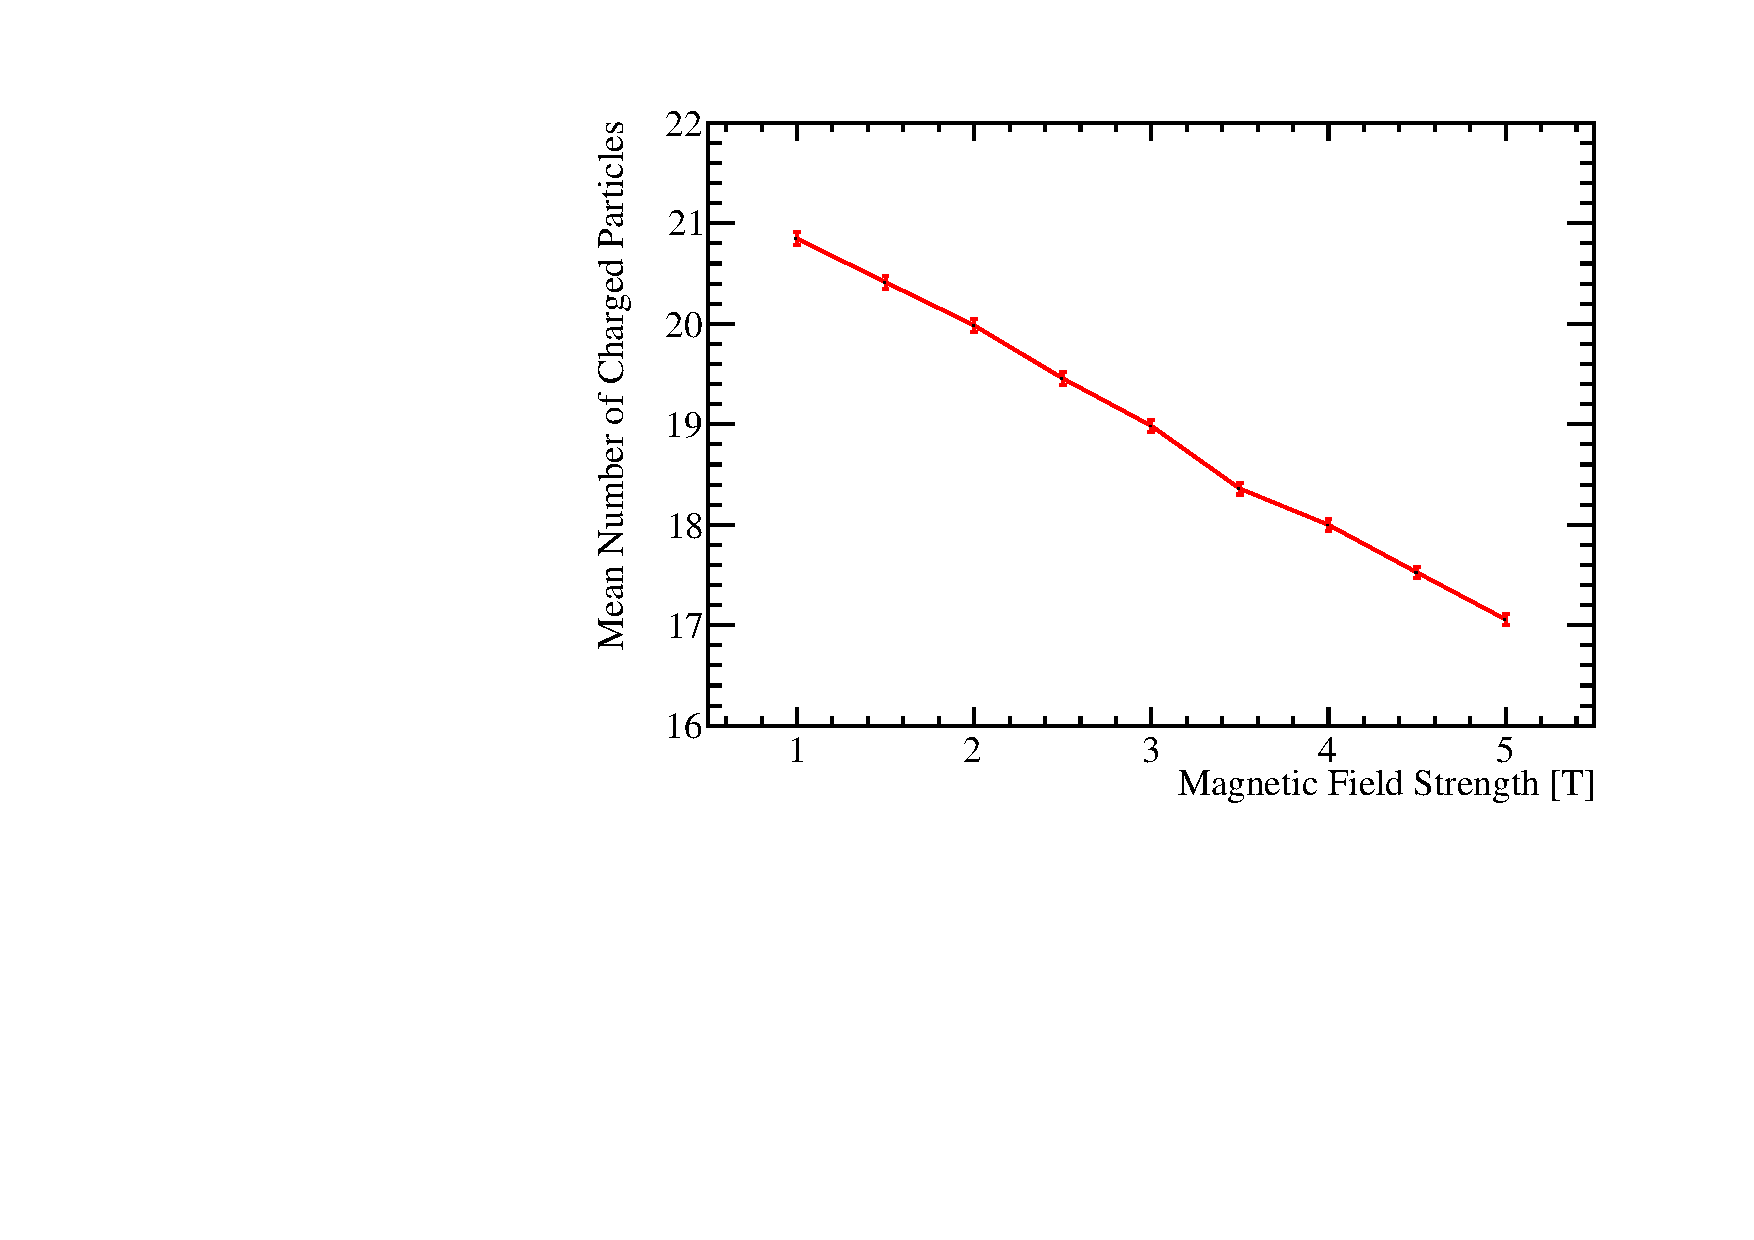
\includegraphics[width=0.5\textwidth]{OptimisationStudies/Plots/Description/BField/BFieldNumbers_91GeV_Z_uds.pdf}
\caption[The mean number of reconstructed charged particles as a function of the magnetic field strength for 91~GeV Z$\rightarrow$uds di-jet events.  The nominal ILD detector model was used and the pattern recognition has been fully cheated using the MC information.]{The mean number of reconstructed charged particles as a function of the magnetic field strength for 91~GeV Z$\rightarrow$uds di-jet events.  The nominal ILD detector model was used and the pattern recognition has been fully cheated using the MC information.}
\label{fig:bfieldchargedparticles}
\end{figure}

In summary, increasing the magnetic field strength is beneficial to detector performance as it reduces confusion from associating tracks to calorimetric energy deposits from charged particles.  While there is a reduction in the intrinsic energy resolution for low transverse momentum jets with increasing magnetic field strength, this effect is largely offset by the change in confusion.  While the nominal field of 3.5 T gives good performance increasing the field strength is a clear way of making gains in detector performance.

%========================================================================================

\subsection{Inner ECal Radius}
Detector models were considered where the ECal inner radius was set to 1208, 1408, 1608, 1808 (nominal) and 2008~mm.  For these models, all other detector parameters were identical to those found in the nominal ILD detector model.

Figure \ref{fig:ecalinnerr} shows the dependence of the jet energy resolution on the ECal inner radius.  The simulations indicate that a large ECal inner radius was highly beneficial to detector performance, which is due to the increase in the time it takes for particles to reach the calorimeters.  The longer it takes for the particles to reach the calorimeters the more the charged particles will bend in the magnetic field and the larger separation will be between calorimetric energy deposits from charged and neutral particles.  This larger this separation the smaller the effect of confusion.  This conclusion is backed up by the decomposition of the jet energy resolution, shown in figure \ref{fig:ecalinnerrbreak}.  These results explicitly show a reduction in confusion with increasing ECal inner radius.  The intrinsic energy resolution of the detectors shows no strong dependence on the inner ECal radius.  There is a small degradation in intrinsic energy resolution at low ECal inner radii, which is due to the association of a single MC particle per calorimeter cell when running the cheated pattern recognition as explained in section \ref{sec:bfield}.  Again, this effect has little bearing on the final conclusions as the change in intrinsic energy resolution across the detector models is a second order effect.  

\begin{figure}[h!]
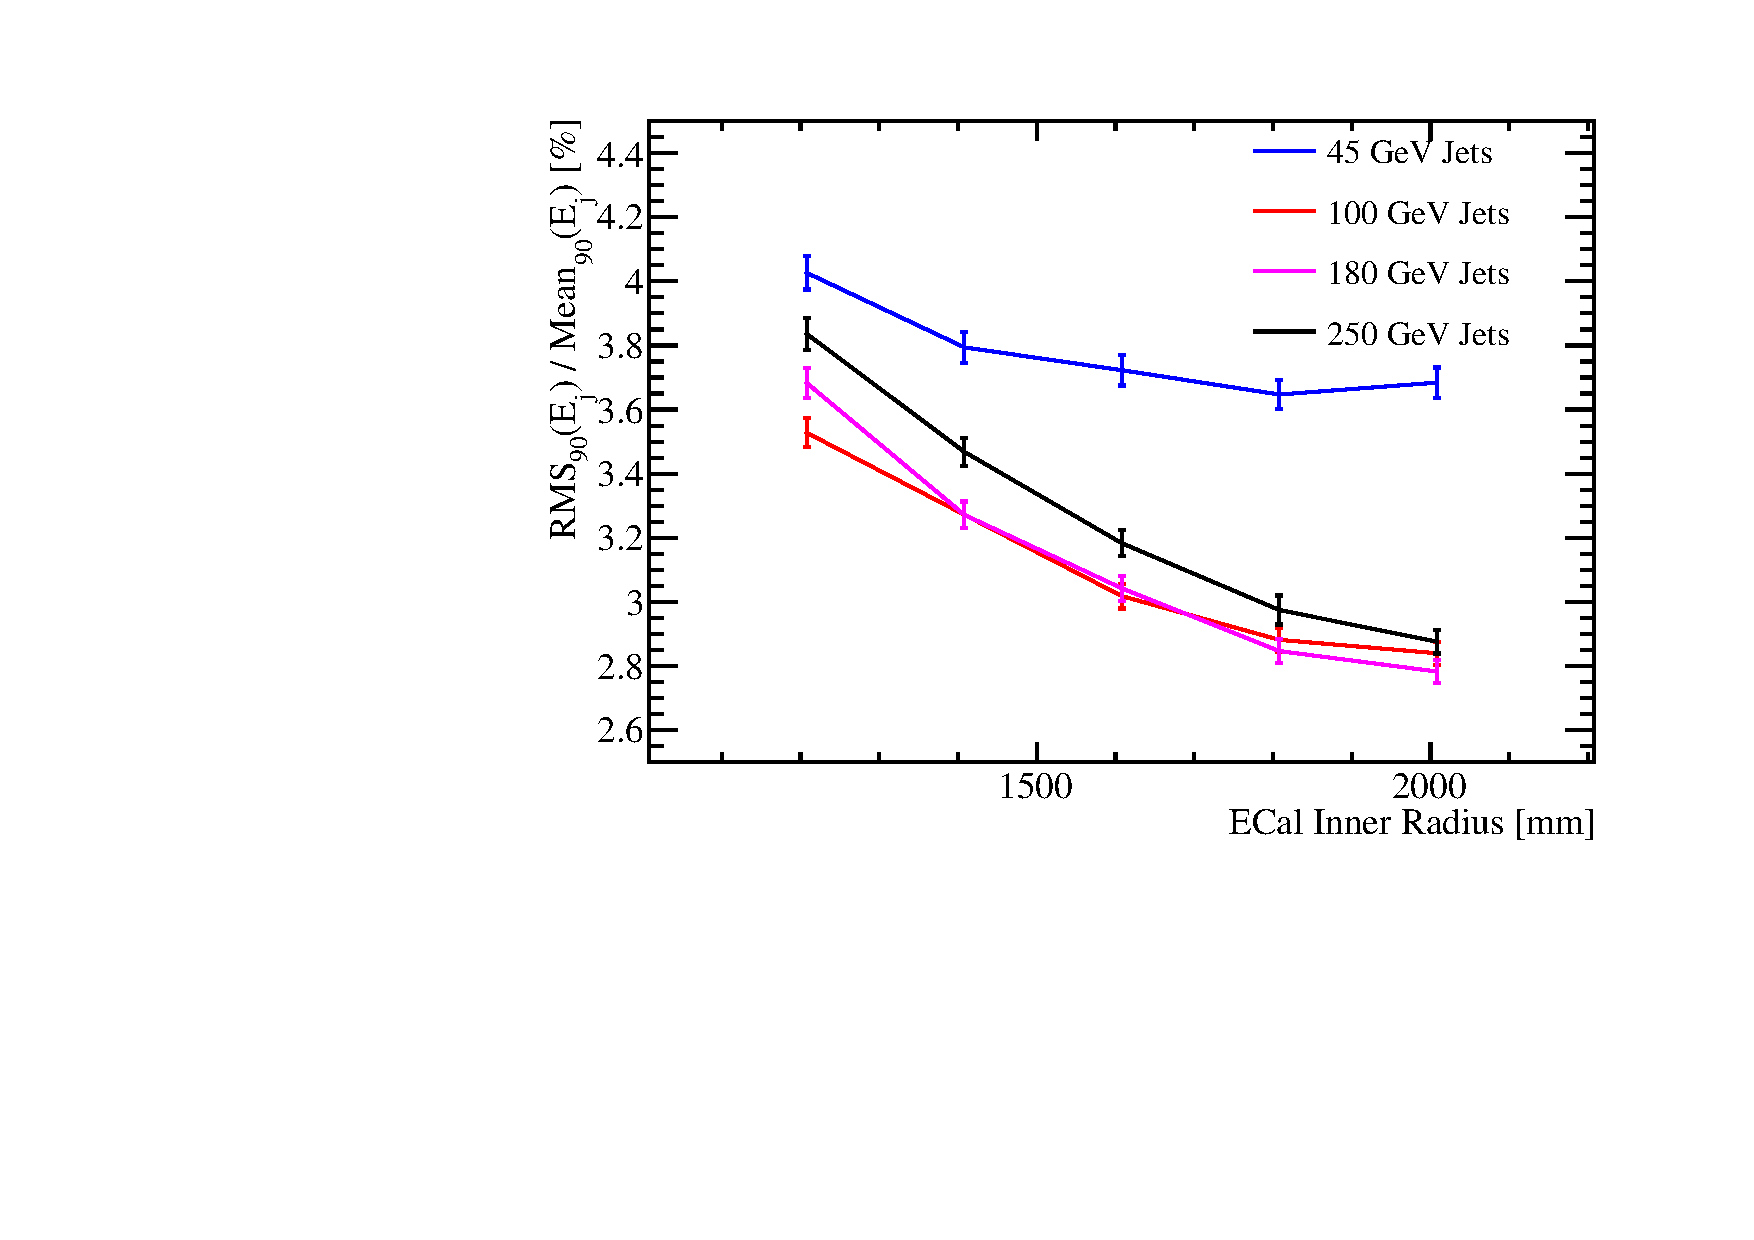
\includegraphics[width=0.5\textwidth]{OptimisationStudies/Plots/JetEnergyResolutions/JER_vs_ECalInnerRadius.pdf}
\caption[The jet energy resolution using the nominal ILD detector as a function of the ECal inner radius for various jet energies.]{The jet energy resolution using the nominal ILD detector as a function of the ECal inner radius for various jet energies.}
\label{fig:ecalinnerr}
\end{figure}

\begin{figure}[h!]
\subfloat[]{\label{fig:ecalinnerr45break}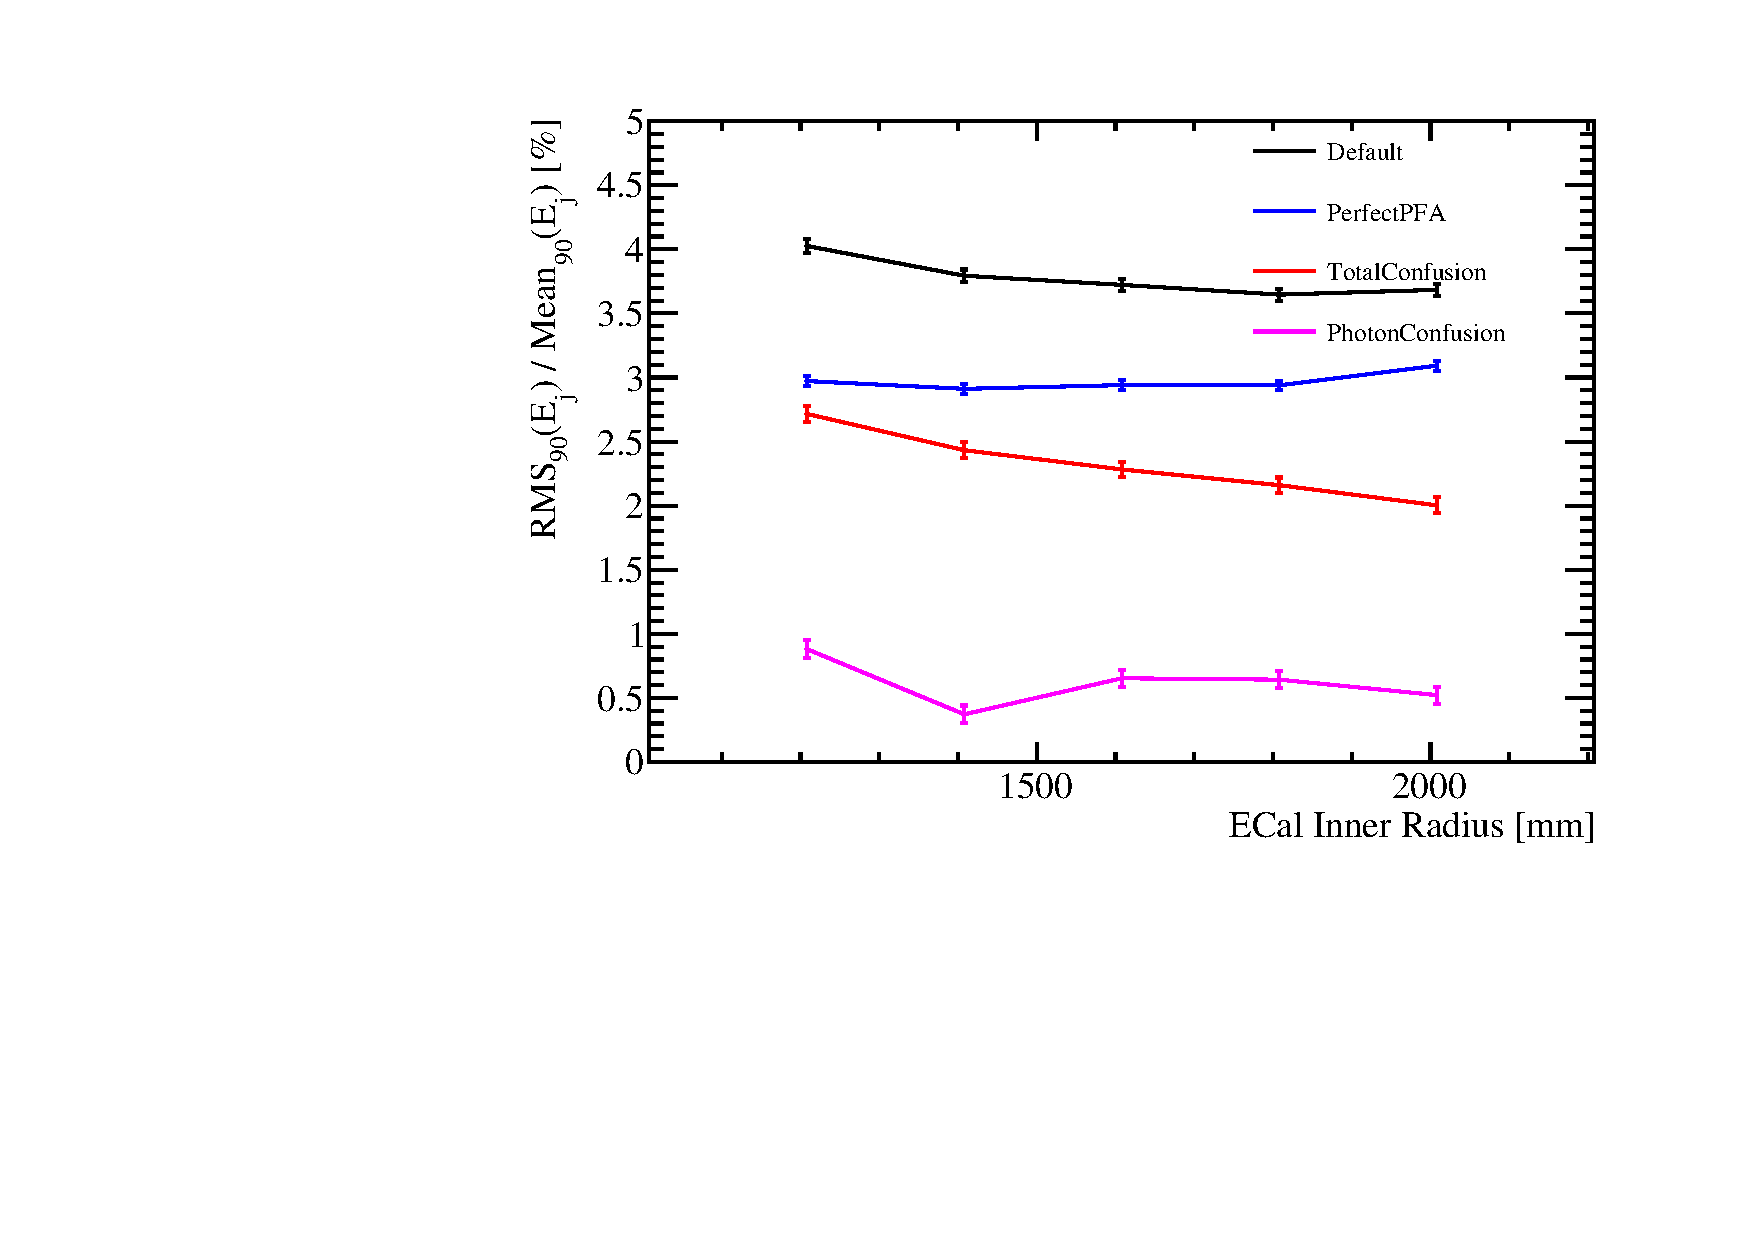
\includegraphics[width=0.5\textwidth]{OptimisationStudies/Plots/JetEnergyResolutions/JER_vs_ECalInnerRadius_91GeV_DiJet_Breakdown.pdf}}
\subfloat[]{\label{fig:ecalinnerr250break}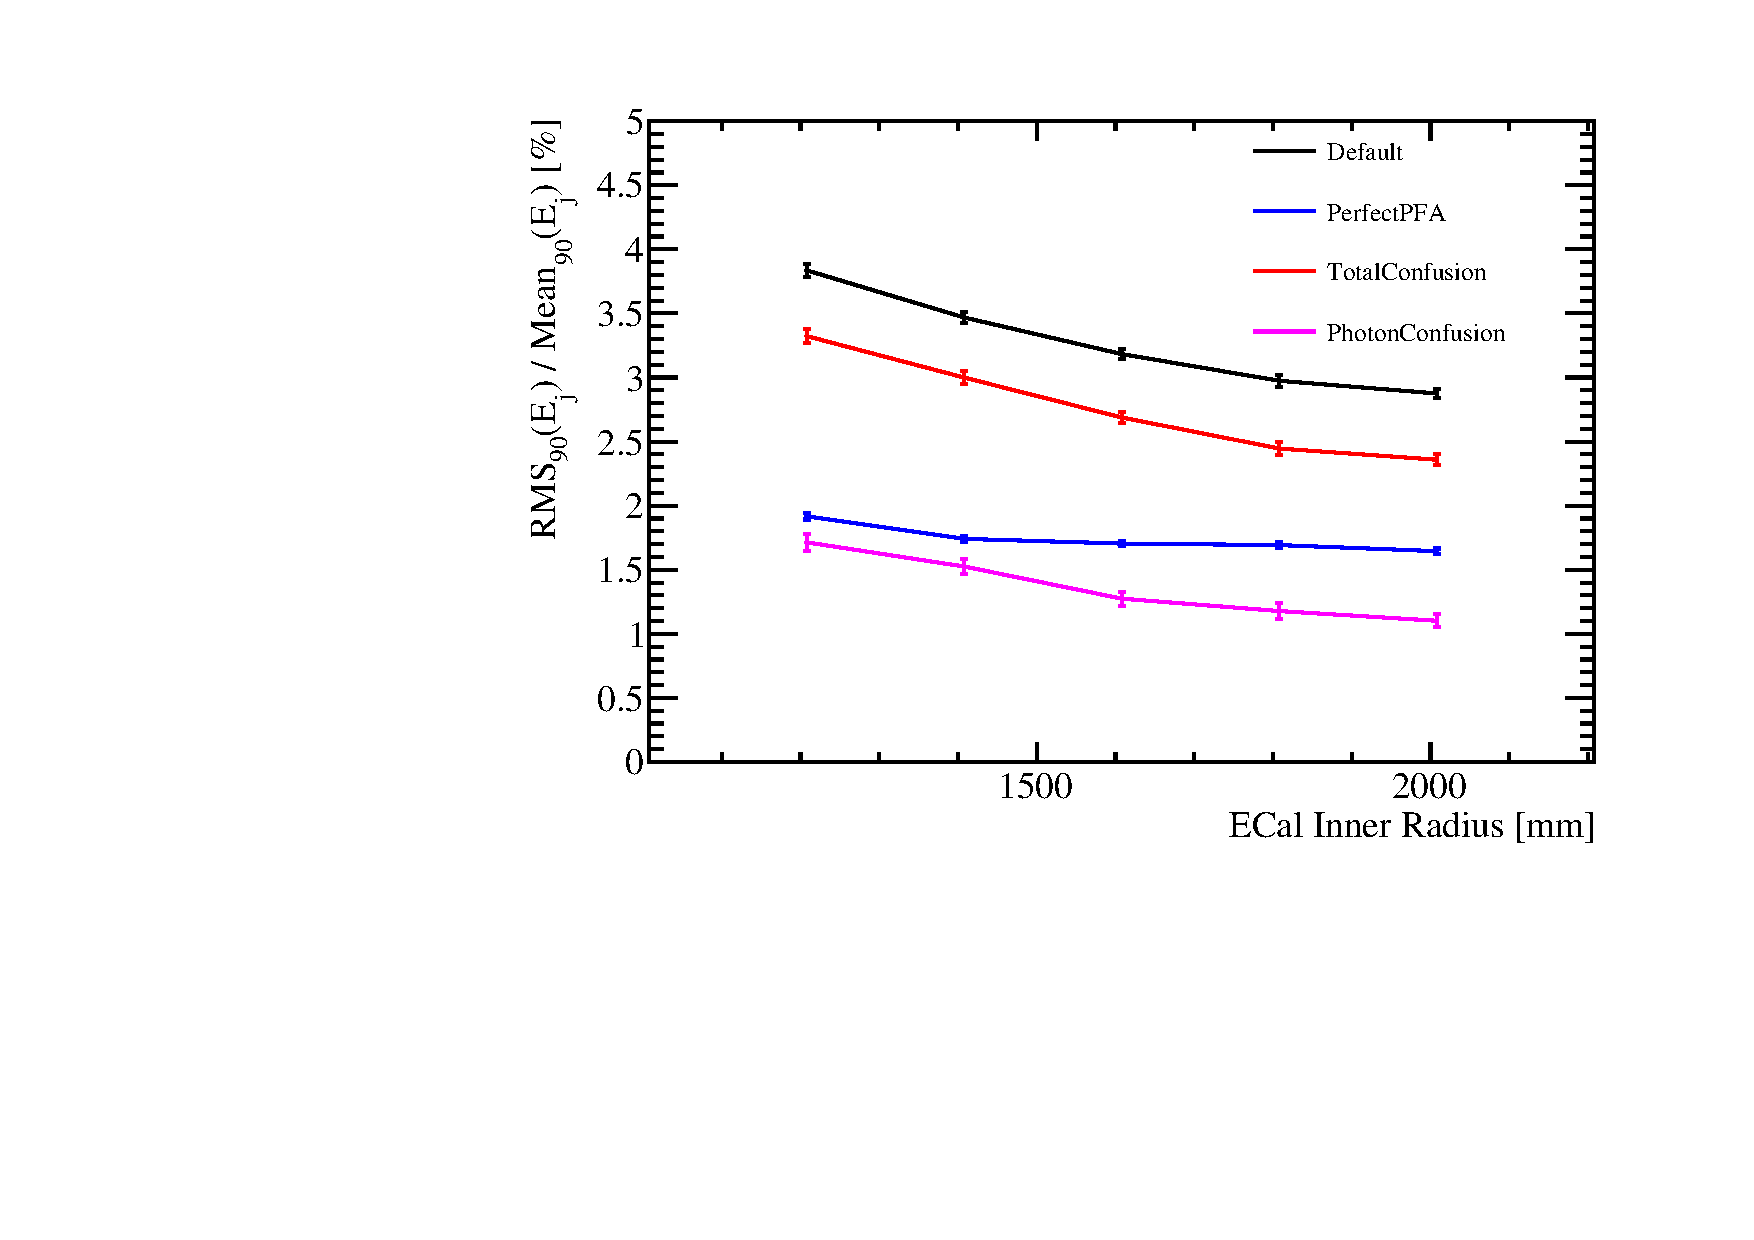
\includegraphics[width=0.5\textwidth]{OptimisationStudies/Plots/JetEnergyResolutions/JER_vs_ECalInnerRadius_500GeV_DiJet_Breakdown.pdf}}
\caption[The contributions to the jet energy resolution as a function of the ECal inner radius using the nominal ILD detector model for \protect\subref{fig:ecalinnerr45break} 45~GeV jets and \protect\subref{fig:ecalinnerr250break} 250~GeV jets.  The black curves correspond to the standard reconstruction, the blue curves to the intrinsic energy resolution contribution to the jet energy resolution, the red curves to the confusion contribution to the jet energy resolution and the magenta curves to the confusion contribution to the jet energy resolution related solely to $\gamma$ reconstruction.]{The contributions to the jet energy resolution as a function of the ECal inner radius using the nominal ILD detector model for \protect\subref{fig:ecalinnerr45break} 45~GeV jets and \protect\subref{fig:ecalinnerr250break} 250~GeV jets.  The black curves correspond to the standard reconstruction, the blue curves to the intrinsic energy resolution contribution to the jet energy resolution, the red curves to the confusion contribution to the jet energy resolution and the magenta curves to the confusion contribution to the jet energy resolution related solely to $\gamma$ reconstruction.}
\label{fig:ecalinnerrbreak}
\end{figure}

In conclusion, increasing the ECal inner radius benefits the jet energy resolution significantly.  This trend is driven by changes to the confusion in associating calorimetric energy deposits to charged particle tracks.  
